%!TEX TS-program = xelatex
%!TEX encoding = UTF-8 Unicode

% Figures: full: 174 mm, letters Myriad Variable Concept Regular 16 pt
% half: 85 mm
% Regular type between 10 and 12 pt

\documentclass{Dissertate}

% TODO notes
\definecolor{lightmauve}{RGB}{230,0,230}
\setlength{\marginparwidth}{2.5cm}
\usepackage[textsize=small, linecolor=mauve, bordercolor=black,
            backgroundcolor=lightmauve]{todonotes}
            
\usepackage{wrapfig}

% Scientific notation in text command
\newcommand{\e}[2]{\num{#1}E\num[minimum-integer-digits=2]{#2}}

%hyphenation shorthand
\usepackage[ngerman, english]{babel}
\useshorthands{"}
\addto\extrasenglish{\languageshorthands{ngerman}}

% full page figure
\usepackage{fltpage}

% math non-italic
%\usepackage[LGRgreek]{mathastext}
%\usepackage{mathastext}
\usepackage{upgreek} %text greek letters

% table cells
\usepackage{makecell}

% Environment for methods
\newenvironment{method}
	{
	\vspace{6pt}
	\begin{sffamily}
	\begin{spacing}{\dcompressedspacing}
	\sisetup{detect-all}
	}
	{
	\end{spacing}
	\end{sffamily}
	\vspace{6pt}
	}

% small similar sign
\newcommand{\smallsim}{\smallsym{\mathrel}{\sim}}

\makeatletter
\newcommand{\smallsym}[2]{#1{\mathpalette\make@small@sym{#2}}}
\newcommand{\make@small@sym}[2]{%
  \vcenter{\hbox{$\m@th\downgrade@style#1#2$}}%
}
\newcommand{\downgrade@style}[1]{%
  \ifx#1\displaystyle\scriptstyle\else
    \ifx#1\textstyle\scriptstyle\else
      \scriptscriptstyle
  \fi\fi
}
\makeatother

% same with gtrsim
\newcommand{\smallgtrsim}{\smallgtrsym{\mathrel}{\gtrsim}}

\makeatletter
\newcommand{\smallgtrsym}[2]{#1{\mathpalette\make@small@gtrsym{#2}}}
\newcommand{\make@small@gtrsym}[2]{%
  \vcenter{\hbox{$\m@th\downgrade@style#1#2$}}%
}
\makeatother

% Items more compact
\usepackage{enumitem}

% Box environment
\usepackage{newfloat}
\DeclareFloatingEnvironment[within=none, fileext=frm, placement={!hb}, name=Box]{boxenv}
\captionsetup[boxenv]{font=normalsize, labelfont=bf, textfont=sf} %labelfont %textfont %font ?
\usepackage[framemethod=TikZ]{mdframed}
\definecolor{shadecolor}{RGB}{143,177,196}
\definecolor{dkshadecolor}{RGB}{51,99,125}
\newenvironment{mybox}[1]
    {
    	\begin{boxenv}[!b]
	\begin{small}
    	\begin{mdframed}[
		%roundcorner=5pt, 
		backgroundcolor=shadecolor, 
		linecolor=dkshadecolor,
  		linewidth=4pt,
  		topline=false,
  		rightline=false,
  		leftline=false
		]
    	\caption{#1}
    }
    {
    	\end{mdframed}
	\end{small}
    	\end{boxenv}
    }

% prevent breaking inside LA-N
\usepackage[shortcuts]{extdash}

% siunitx number format
\sisetup{detect-all}

% diagonal fractions
% \usepackage{xfrac}
            
% acronyms
%!TEX root = dissertation.tex

\DeclareAcronym{a7}{
short = CHRNA7,
long = nicotinic acetylcholine receptor subunit $\alpha7$,
class = abb,
sort = chrn
}
\DeclareAcronym{ach}{
short = ACh,
long = acetylcholine,
class = abb
}
\DeclareAcronym{ache}{
short = ACHE,
long = acetylcholinesterase,
class = abb
}
\DeclareAcronym{ago}{
short = Ago,
long = argonaute,
class = abb
}
\DeclareAcronym{api}{
short = API,
long = application programming interface,
class = abb
}
\DeclareAcronym{cage}{
short = CAGE,
long = 5' cap analysis of gene expression,
class = abb
}
\DeclareAcronym{chat}{
short = CHAT,
long = choline acetyltransferase,
class = abb
}
\DeclareAcronym{cns}{
short = CNS,
long = central nervous system,
class = abb
}
\DeclareAcronym{cntf}{
short = CNTF,
long = ciliary neurotrophic factor,
class = abb
}
\DeclareAcronym{cntfr}{
short = CNTFR,
long = ciliary neurotrophic factor receptor (soluble),
class = abb
}
\DeclareAcronym{ilst}{
short = IL6ST,
long = interleukin 6 signal transducer (membrane bound); also known as gp130,
class = abb
}
\DeclareAcronym{jak}{
short = JAK,
long = janus kinase,
class = abb
}
\DeclareAcronym{gp}{
short = gp130,
long = see IL6ST,
class = abb
}
\DeclareAcronym{il}{
short = IL-6,
long = interleukin 6,
class = abb
}
\DeclareAcronym{ilr}{
short = IL6R,
long = interleukin 6 receptor (soluble),
class = abb
}
\DeclareAcronym{lif}{
short = LIF,
long = leukaemia inhibiting factor,
class = abb
}
\DeclareAcronym{lifr}{
short = LIFR,
long = leukaemia inhibiting factor receptor (soluble),
class = abb
}
\DeclareAcronym{mir}{
short = miRNA,
long = microRNA,
class = abb
}
\DeclareAcronym{ngf}{
short = NGF,
long = nerve growth factor,
class = abb
}
\DeclareAcronym{risc}{
short = RISC,
long = RNA-induced silencing complex,
class = abb
}
\DeclareAcronym{slc}{
short = SLC18A3,
long = vesicular acetylcholine transporter (official gene symbol),
class = abb
}
\DeclareAcronym{sql}{
short = SQL,
long = structured query language,
class = abb
}
\DeclareAcronym{stat}{
short = STAT,
long = signal transducer and activator of transcription,
class = abb
}
\DeclareAcronym{tf}{
short = TF,
long = transcription factor,
class = abb
}
\DeclareAcronym{trf}{
short = tRF,
long = transfer RNA fragment,
class = abb
}
\DeclareAcronym{tirna}{
short = tiRNA,
long = transfer RNA half,
long-plural-form = transfer RNA halves,
class = abb
}
\DeclareAcronym{trna}{
short = tRNA,
long = transfer RNA,
class = abb
}
\DeclareAcronym{tyk}{
short = TYK,
long = tyrosine kinase,
class = abb
}
\DeclareAcronym{utr}{
short = UTR,
long = untranslated region,
class = abb
}
\DeclareAcronym{vacht}{
short = vAChT,
long = vesicular acetylcholine transporter,
class = abb
}

\begin{document}

% the front matter
%!TEX root = ../dissertation.tex
% Some details about the dissertation.
\title{Small RNA dynamics in cholinergic systems}
\author{Sebastian Lobentanzer}

%If you have one advisor
\advisor{Jochen Klein}

%If you are coadvised
\coadvisorOne{Hermona Soreq}

% ... about the degree.
\degreeyear{2019-2020}

% \maketitle
% \copyrightpage
\frontmatter
\renewcommand{\chapterheadstartvskip}{\vspace*{-0.5\baselineskip}} %this shifts chapter headlines vertically
\setstretch{\dnormalspacing}
% \abstractpage
% \tableofcontents
% %\authorlist
% \listoffigures
% \dedicationpage
% \acknowledgments

% \doublespacing


% include each chapter...
% \setcounter{chapter}{-1}  % start chapter numbering at 0
%!TEX root = ../dissertation.tex
\chapter{Introduction}
\label{introduction}

%!TEX root = ../dissertation.tex
\section{Cholinergic Systems}
\newthought{Nary a process in the mammalian body can commence without participation of cholinergic systems.} \Ac{ach} was chemically and pharmacologically described by Henry Dale more than 100 years ago.\cite{Dale1914} A short time later, Otto Loewi published the first proof of signal transmission by small molecules: he transferred physiological solutions from electrically stimulated frog hearts to naive hearts and observed their reactions; the solution that provoked a parasympathetic response he proposed to contain a »vagus substance«.\cite{Loewi1921} Finally, in 1929, Henry Dale completed the picture by isolating acetylcholine from mammalian tissue and identifying it as the molecule responsible for the parasympathetic response.\cite{Dale1929} Dale and Loewi's joint effort in »Discoveries Relating to Chemical Transmission of Nerve Impulses« was rewarded with the »Nobel Prize in Physiology or Medicine« in 1936.

Although we have learned much about cholinergic systems in these past 100 years, our understanding of the mammalian nervous system still is fairly limited. Even when disregarding peripheral nervous systems, the complexity of cholinergic transmission is immense, and a myriad functions have been attributed to cholinergic circuits in the \ac{cns}. Central nervous projections of cholinergic fibres were extensively mapped by Marek-Marsel Mesulam and others in the 1980s,\cite{Mesulam1984, Mesulam1988} with a majority of long projection neurons originating in one of the eight cholinergic nuclei, Ch1-Ch8. While many of these anatomical structures have been filled with meaning by associations with both rudimentary as well as higher brain functions, there are still as many cholinergic pathways whose function is entirely unclear (Figure \ref{fig:projections}, from Lobentanzer \emph{et al.}\cite{Lobentanzer2019a}). This holds particularly true for the only recently discovered cortical cholinergic interneurons, which, in comparison to their projecting counterparts, are very small and numerically vastly inferior to other neuron types in the cortex. Thus, their detection and analysis with current methods is challenging. 

\begin{figure}
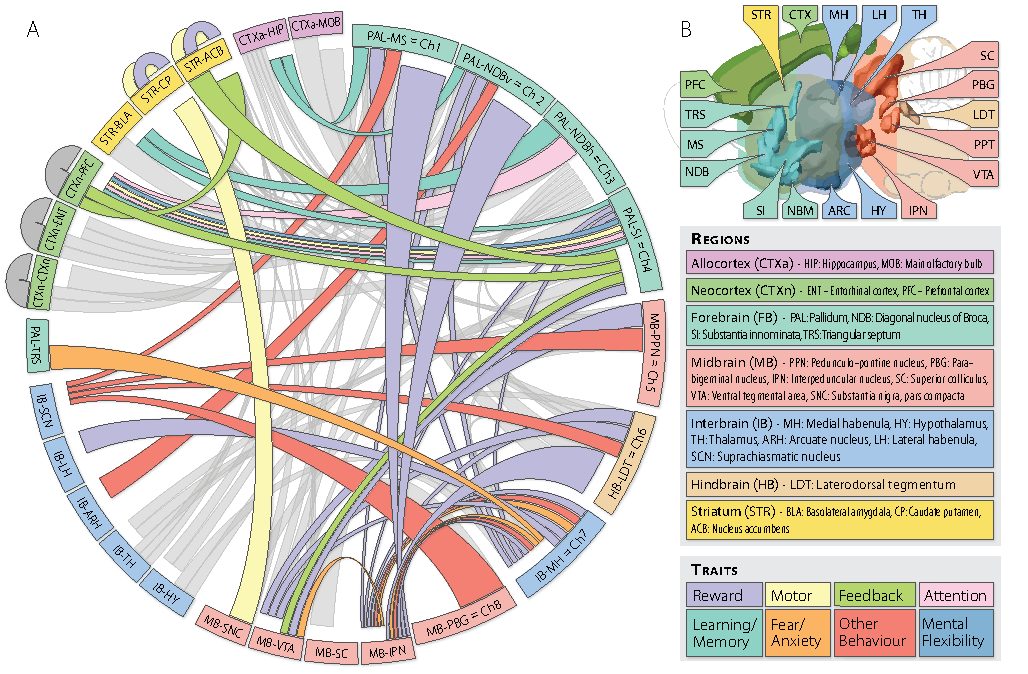
\includegraphics[width=\textwidth]{figures/projections}
\caption[Cholinergic Projections.]{\textbf{Cholinergic Projections in the CNS.} Cholinergic systems are implicated in many diverse functional categories. \textbf{A)} The bulk of cholinergic projection neurons stems from one of the eight cholinergic nuclei, Ch1-Ch8 (right side of ideogram). They innervate wide areas of the mammalian CNS, and in turn receive incoming connections from all around the brain (left side of ideogram). Efferent connections are indicated by a small gap between ideogram and connector, in the first clockwise half of each ideogram component, afferent connection by a large gap, in the second half. A number of projections has been associated with specific functions, as implicated by the colours of the connectors. Two populations of cholinergic interneurons have been identified, in the striatum and the neocortex (outside of ideogram). \textbf{B)} Brain region and trait colour legend for A).
\label{fig:projections}}
\end{figure}

The histological definition of what constitutes a cholinergic neuron is not without debate. The staining procedures established in the 1970s utilised monoclonal antibodies against \ac{achep},\cite{Mesulam1976} whose association with cholinergic neurons is not definitive, as it can be expressed post-synaptically as well (for an overview of genes of the cholinergic systems, see Box \ref{box:chol-genes}). Later on, developments in horseradish peroxidase systems allowed immunohistochemistry on \ac{chatp}, which is a more immediate marker of cholinergic neurons,\cite{Mesulam1984} albeit much more lowly expressed than AChE. However, AChE-based staining still was consistently used in addition to ChAT staining,\cite{Mesulam1988} sometimes without much differentiation. Recently, single-cell \ac{seq} allows a more detailed appreciation of the transcriptional diversity of neurons, and enables a clearer distinction between cholinergic and non-cholinergic neurons expressing AChE (see Section \ref{sec:cellculture:singlecell}).

\begin{mybox}{The Cholinergic Genes}\label{box:chol-genes}
Acetylcholine is synthesised from acetyl-CoA - supplied by \textbf{ATP citrate lyase} (\emph{ACLY}) - and choline via enzymatic catalysis by \textbf{choline acetyltransferase} (ChAT from the \emph{CHAT} gene). It is then packed into vesicles by the \textbf{vesicular acetylcholine transporter} (vAChT from the \emph{SLC18A3} gene). After release into the synaptic cleft, it binds to a variety of \textbf{nicotinic and muscarinic receptors} (\emph{CHRNx}, 16 subunits, and \emph{CHRMx}, 5 subtypes). Of those, the nicotinic receptors form heteropentameric or, seldom, homopentameric ion channels, while the muscarinic receptors are monomeric G protein-coupled transmembrane receptors. The human possesses a duplicate of the nicotinic $\upalpha$7 receptor, \textbf{dup$\upalpha$7} (\emph{CHRFAM7A}), which cannot bind ACh and supposedly acts as a dominant negative regulator of the $\upalpha$7 homomeric receptor. Termination of the signal is mainly achieved by \textbf{acetylcholinesterase} (AChE from the \emph{ACHE} gene), one of the fastest enzymes known, with a theoretical rate of \num{25000} molecules per second. AChE tetramers are usually tethered to cell membranes in the synaptic vicinity by the \textbf{proline-rich membrane anchor} (\emph{PRIMA1}) or \textbf{collagen Q} (\emph{COLQ}) peptides. Complementary to the mostly residual AChE is the circulatory \textbf{butyryl cholinesterase} (BChE from the \emph{BCHE} gene), which can also nonspecifically degrade ACh. After degradation, residual choline is reimported into cells via the \textbf{high affinity choline uptake transporter} (HACU, from the \emph{SLC5A7} gene).
\end{mybox}

\section{Cholinergic Aspects of Physiology and Disease} \label{sec:intro:diseases}
\newthought{Cholinergic systems are integral} for a myriad physiological functions, and as such they are critically involved in aetiologies and phenotypes of a number of central and peripheral diseases. Of interest to this dissertation are the cholinergic aspects of degenerative and non-degenerative central nervous diseases (such as Alzheimer's Disease, Bipolar Disorder, Schizophrenia), ischemic conditions in stroke, and peripheral modulation of immune responses, particularly in the context of the aforementioned diseases.

\subsection{Alzheimer's Disease}
\ac{ad} was characterised by Alois Alzheimer in 1906 and later named after him by his colleague and mentor, Emil Kraepelin.\cite{Berrios1990} AD is a progressive neurodegenerative disease, its main risk factor is age, and it is estimated to make up 60-70\% of all dementia cases. The disease incidence and progression distinctly differ between the sexes;\cite{Miech2002} generally, women are affected more often. Unlike the very rare familial form (that can affect patients in their fifties), spontaneous AD usually only begins to manifest symptomatically in the 6th to 7th life decade. As a result of the demographic change in most western countries, patient numbers, and thus, medical efforts, are expected to more than double in size until the year 2050. The cognitive decline associated with AD is progressive and ultimately leads to exhaustive care dependency; there is no cure.

The pathological hallmarks of AD are two types of atypical protein aggregates, inter-cellular amyloid $\upbeta$ »plaques«, and intra-cellular »neurofibrillary tangles« composed of hyper-phosphorylated tau-protein. Often, pathological aggregation of these proteins begins decades before the onset of symptoms. However, there have also been numerous cases of cognitively healthy subjects showing high amounts of protein aggregates. These inconsistencies and the unclear causality of pathology and symptoms have led to a redirection of scientific efforts to processes unrelated to amyloid and tau, such as neuroinflammation.

Cholinergic systems have long been associated with AD, as evidenced by the cholinergic hypothesis that was posed in the 1980s. To cite from Bartus \emph{et al.}, 1982:\cite{Bartus1982}

\begin{quote}
»We have been guided by three deductive requirements that must be satisfied if the cholinergic hypothesis is to deserve continued attention: (i) specific dysfunctions in cholinergic markers should be found in the brains of subjects suffering from age-related memory loss, (ii) artificial disruption of central cholinergic function in young subjects should induce behavioural impairments that mimic the cognitive loss found naturally in aged subjects, and (iii) appropriately enhancing central cholinergic activity in aged subjects should significantly reduce age-related cognitive deficits.«
\end{quote}

Although many reports substantiate all three deductive prerequisites, the cholinergic hypothesis has in the last decades been overshadowed by alternative hypotheses, particularly, amyloid-related theories. However, the therapeutic approaches developed along the lines of preventing amyloid $\upbeta$ aggregation or otherwise clearing the plaques or soluble aggregates have not been successful in alleviating the cognitive decline in patients(cite). Thus, pro-cholinergic intervention by means of \ac{achep} inhibition still makes up the majority of approved drugs. The monotherapeutic approach of AChE inhibition is based on a premise that seems simple in light of the enormous complexity surrounding the interplay of the billions of neurons in the process of memory formation and recall, and in fact, pro-cholinergic therapy has only been shown to alleviate symptoms or delay their onset; a reversal of cognitive losses has so far not been achieved by any drug regime. As such, even in regard only to the cholinergic systems, novel approaches are sorely needed.

On the other hand, the cholinergic deficit in AD is not purely symptomatic. There is considerable debate whether the pathology originates from the entorhinal cortex or the basal forebrain. As Heiko and Eva Braak have shown,\cite{Braak1995} AD pathology follows a characteristic brain region distribution process that can be stratified into stages and starts in the entorhinal region. The early stages of pathology by far precede the onset of symptoms. Taylor Schmitz and colleagues substantiate the cholinergic origin of neurodegeneration in their longitudinal \emph{in vivo} imaging studies:\cite{Schmitz2016, Schmitz2018} In cognitively normal and impaired human subjects, basal forebrain volume predicted longitudinal entorhinal degeneration, but not \emph{vice versa}. As such, the cholinergic basal forebrain dysfunction precedes as well as predicts pathology in other affected areas and cognitive deficits.\cite{Schmitz2016} Additionally, the spread of Alzheimer's pathology in the longitudinal progression of the disease reflects the spatial topography of basal forebrain cholinergic projections.\cite{Schmitz2018}

% sexual dimorphism in response to ache inhibitors Giacobini2018

%Li Gan - NFkB activation by tau
% - Ikkbeta knockout corrects STAT1 DE

\subsection{Schizophrenia and Bipolar Disorder} 
Cognitive deficits can also occur without neuron death. The earliest description of what we today call \ac{scz} was coined by Emil Kraepelin: »\emph{dementia praecox}«, premature dementia.\cite{Kraepelin1913} Cognitive deficits are an integral but often overlooked part of the clinical picture of SCZ, which is often dominated by the more impressive positive symptoms such as hallucinations and paranoia. Likewise, \ac{bd} can present with cognitive impairments. The cognitive impairments affecting both SCZ and BD patients involve diminished problem solving capabilities and reduced intelligence, and are more pronounced in SCZ than in BD.\cite{Bortolato2015} They have been connected to cholinergic dysfunction\cite{VanEnkhuizen2015, Smucny2017} and the sum of anticholinergic medications.\cite{Gray2015, Eum2017} A human polymorphism in the $\upalpha$5 nicotinic receptor subunit predicts a higher propensity for smoking and SCZ, showing parallel manifestations in engineered mice\cite{Koukouli2017} and rats.\cite{Forget2018} Correspondingly, cholinergic stimulation can improve cognition\cite{Sacco2004, Rowe2015, Lewis2017} and mood,\cite{Higley2014} but can on the other hand provoke schizotypic behaviour in AD patients.\cite{Degirmenci2016}

SCZ and BD clinically present with clear sexual dimorphisms. Compared to women, men have a higher SCZ prevalence with an \ac{or} of 1.4, are affected earlier (at 15-25 as compared to 25-35 years of age), and face a worse prognosis.\cite{Leger2016} Cholinergic participation also appears sex-dependent: Male SCZ patients more often self-medicate by smoking (7.2 versus 3.3 weighted average OR with 90\% lifetime prevalence).\cite{DeLeon2005} BD, on the other hand, affects men and women almost equally, with an OR of $\smallsim$\num{1}. However, women make up 80-90\% of so-called »rapid cyclers«, a subgroup of patients showing short intervals between manic and depressive phases which is associated with a worse prognosis.\cite{Berger2014} Additionally, major depressive disorder, which is a prerequisite for BD diagnosis, more often affects women\cite{Berger2014} (OR = 2).

Psychiatric genomics has recently identified a high amount of shared heritability between SCZ and BD.\cite{Anttila2018} Likewise, transcriptomic analyses have shown a high correlation (71\%) between the transcriptional perturbations in the two diseases.\cite{Gandal2018} Clinical as well as molecular pathology intensifies from BD to SCZ, suggesting the two lie on different points of a shared spectrum. However, their genetic origins are tremendously complex. Multiple disease-relevant markers have been identified by GWAS (genome-wide association studies), even able to distinguish between several sub-phenotypes of each disease.\cite{Ruderfer2018} These markers are found in neurotransmitter receptors (e.g., dopaminergic, glutamatergic, cholinergic), scaffolding proteins (DISC: »disrupted in schizophrenia«), multiple \acp{tf}, \acp{mir}, and non-coding regions without known function.\cite{Harrison2015, Henriksen2017, Kanazawa2017}

Considering this complex disease aetiology, it is not surprising that there are no »designer« drugs available against SCZ and BD. All available therapeutic options have been empirically found, starting with the first antipsychotic, chlorpromazine, synthesised in 1950 by the French pharmaceutical company Rhône-Poulenc. Originally developed in a series dedicated to the search for antihistaminics, it was soon recognised for its antipsychotic potential, and widely prescribed only few years later. Many other neuroleptic compounds have been derived from chlorpromazine, and through binding affinity assays, their receptor profiles were established. Most compounds with antipsychotic properties have a wide spectrum of different receptor activities, but most early drugs were strong antagonists of the D$_2$ dopamine receptor. Thus, the »dopaminergic hypothesis« of SCZ was formulated. However, aetiology as well as therapeutic principles are unclear to this day, and most antipsychotic substances still are very »dirty drugs«. In fact, newer developments leading to the discovery of the second generation (»atypical«) neuroleptic substances, starting with clozapine, have created molecules with an even wider spectrum of interactions und thus less specificity towards a single therapeutic mechanism of action. Similarly, the archetypal »mood stabiliser« Lithium, that has been found to ameliorate depressive as well as manic phases of BD, likely influences a wide variety of neuronal functions via mechanisms yet unclear.\cite{Malhi2013} This general development is contrary to pharmaceutical research practice, where most developments aim for a higher specificity. It is thus very likely that pharmacological therapy of SCZ and BD requires an approach consisting of multiple pharmacodynamic angles, to account for the multigenic disruption.

\subsection{Immunity} \label{sec:intro:immunity}
Aside from its vast neuronal functions, \ac{ach} also is highly relevant in immune cells, recently reviewed by Fujii and colleagues.\cite{Fujii2017} The first to isolate ACh from an animal organ, Dale and Dudley,\cite{Dale1929} used the spleens of oxen and horses. The spleen receives sympathetic, but not parasympathetic innervation, and as such, the ACh found by Dale and Dudley had to have come from immune cells. Indeed, nearly all mammalian immune cells express cholinergic components, most importantly, B- and T-cells, macrophages, and dendritic cells. While ACh is physico-chemically rather stable, it is extremely susceptible to enzymatic degradation, and cholinesterases are ubiquitarily distributed and cleave ACh with stunning efficiency, reducing its diffusion range to few millimetres. As a result, ACh has to be supplied synaptically or, at most, in paracrine fashion. \Ac{chatp} activity has been confirmed in B- and T-cells, which both contain significant amounts of ACh, although T-cells generally possess higher amounts. Additionally, in peripheral cells ACh can be synthesised by the mitochondrial carnitine acetyltransferase. In addition to B- and T-cells, \emph{\acs{chat}} mRNA has been found in macrophages and dendritic cells. \ac{chatp} expression and ACh synthesis can be induced by various immune mediators, such as \ac{lps} and \ac{tlr} agonists.

In addition to ACh synthesis, all of the aforementioned cell types can receive cholinergic signals. They express all muscarinic receptors as well as a selection of nicotinic receptor subunits, and the signal-terminating esterases. Although it is not completely clear how the parasympathetic signal reaches the immune cells, cholinergic activation as a result of inflammation can dampen the immune response in what is described as the »cholinergic anti-inflammatory reflex«.\cite{Pavlov2017} This reflex loop is designed to protect the body from pathogens and inflammation, but also from the harmful effects of immune stimulation. Upon afferent signalling through the afferent vagus nerve and humoral components, the brain releases humoral (via the hypothalamic-pituitary-adrenal axis) and neuronal (via the sympathetic and parasypathetic autonomous fibres) anti-inflammatory signals. The spleen has been identified as a pivotal organ in this response. Since none of the immune organs receives parasympathetic innervation, it has been proposed that the cholinergic activation is generated locally, with the help of sympathetic signalling to the organ.\cite{Dantzer2018}

A special role among cellular ACh receptors is occupied by the $\upalpha$7 nicotinic receptor subunit. Previously thought to exclusively form homopentameric ion-channel receptors, its functional characteristics have recently been extended. It has been found to form heteropentamers with $\upbeta$2 subunits, akin to the prominent $\upalpha$4$\upbeta$2 receptors in the brain, and an expression in immune cells also is likely. A hybrid duplication of the \emph{CHRNA7} gene with \emph{FAM7}, \emph{CHRFAM7A}, is translated to a functional protein (dup$\upalpha$7). However, it seems to lack ACh binding ability, and thus is thought to act as a dominant negative regulator of $\upalpha$7 receptor function. In addition to its ionotropic function, mainly by means of Ca$^{2+}$ transduction, the $\upalpha$7 receptor has been found to possess G-protein coupled metabotropic effects that can extend the duration of cholinergic activation. The $\upalpha$7 receptor can also, independently of Ca$^{2+}$, activate the JAK2/STAT3 pathway (see Section \ref{sec:intro:neurokine}) in macrophages, leading to suppression of \acs{nfkb} signalling.

On the other hand, cholinergic activation via M$_1$ and/or M$_5$ muscarinic receptors can lead to a positive immune response. The difference between muscarinic and nicotinic immune-signalling is elucidated by transgenic receptor \ac{ko} animals: Splenar cells from selective M$_1$/M$_5$-\ac{ko} mice secreted significantly lower amounts of the neuromodulators \ac{tnf}-$\upalpha$, \ac{ifn}-$\upgamma$, and \ac{il}-6 than those from \ac{wt} mice. Conversely, antigen-stimulated splenar cells from $\upalpha$7-\ac{ko} mice produced significantly greater amounts of \ac{tnf}-$\upalpha$, \ac{ifn}-$\upgamma$, and \ac{il}-6 than \ac{wt}. In summary, the effects of cholinergic stimulation of the immune system is bidirectional and strongly context-dependent, and specific pharmacological intervention can shift homeostasis in both pro- as well as anti-inflammatory directions.

\subsection{Neuroinflammation}
Neurodegenerative as well as non-degenerative neurologic diseases are increasingly being associated with immunologic phenomena, prompting the need for integrative and translational approaches.\cite{Lurie2018} Transient and chronic inflammatory events can influence neuronal function and even survival in a dramatic fashion. Further, failure to resolve the acute inflammatory states might lead to maladaptive states, cases of »frustrated resolution«,\cite{Fullerton2016} in which the goal of adaptive immunity is not met. As was recently shown,\cite{Newson2014} resolution of inflammation is not just the »phasing-out« of inflammatory events, but rather bridges the gap between innate and adaptive immunity. While many acute-phase T$_\mathrm{H}$1-type cytokines might have evolved to drive inflammation, their protracted influence may derail these post-inflammatory events and thus lead to maladaptive responses and chronic inflammation. T$_\mathrm{H}$1-type cytokines include \ac{tnf}, \acp{ifn}, IL-1$\upbeta$ and \ac{il}-6, and downstream mediators discussed in this context are manifold: \ac{pi3k}; \ac{camp}; \ac{mcl1}; the complex of \ac{bcl2}, \ac{akt}, and \ac{bad}; all variants of \ac{mapk}, i.e., \ac{erk} 1 and 2, \ac{jnk}, and p38 MAPK; and the \ac{nfkb} pathway. This list is not comprehensive, for a more detailed overview, see Fullerton \& Gilroy.\cite{Fullerton2016}

While none of the cardinal symptoms of inflammation are easily assessed in a \ac{cns} context, Vir"-chow's fifth cardinal sign, \emph{functio laesa}, is particularly difficult to tie to chronic neuroinflammation. Complex behavioural syndromes such as the functional deficits accompanying neurologic diseases might be influenced by protracted, maladaptive immunity, but the affected areas, brain structures, and timelines cannot be measured with current methods in neuroimaging. Only recently, it has become known that the brain is not immunologically pristine, but rather possesses a very specialised immune system, showing grave distinctions from, but also overlap with, peripheral immune systems.\cite{Louveau2015, Negi2018} The mechanisms of immune privilege of the brain are constantly being refined; there is crosstalk between brain and periphery with blood-to-brain and brain-to-blood messaging,\cite{Dantzer2018} and even migration of immune cells into the CNS, mainly as a response to sustained inflammation.

The first line of defence in CNS tissues are microglia, which in physiological state are resident ramified macrophages, and upon antigen sensing can produce an immediate native immune reaction. Further, the nascent immune system of the CNS comprises similar cells as the peripheral systems (T-cells, B-cells, NK-cells, dendritic cells), albeit with significant differences: antigen presenting cells express significantly fewer \ac{mhc} I and II molecules (which can however be induced by cytokine release upon inflammation); and the endocrine conditions (secretion of immune mediators from neurons) entail a more rapid response (seconds instead of days) with shorter duration of inflammation than in the periphery.\cite{Negi2018}

Under the surveillance of resident microglia, there is constitutive and inducible migration of immune cells between CNS tissues and periphery, in a loop of infiltration and drainage. Starting at antigen presentation inside the CNS, activated immune cells leave the CNS through one of two routes, both ending at the deep cervical lymph nodes: either through the cribiform plate into the nasal mucosa, or into the meningeal lymphatic vessels accompanying the sagittal and transversal sinuses in the \emph{dura mater}. Following an immunological stimulus, activated immune cells in the deep cervical lymph nodes facilitate a secondary immune response and protect nervous tissue through secretion of cytokines\cite{Walsh2015} and re-migration of secondary immune cells to the CNS. Regulatory cytokines include IL-1 and IL-6, CCLs and CXCLs, \ac{lif}, and epidermal and fibroblast growth factors. Re-migrating T cells can utilise various adhesion molecules expressed by endothelia along the blood-brain-barrier to cross into the CNS in a controlled fashion.\cite{Negi2018}

%Sabatino?\cite{Sabatino2019}

%The remarkable saga of the anti-inflammatory cholinergic reflex proposed by Kevin Tracey in the 2000s illustrates very well the various ingredients of the controversy about the parasympathetic innervation of lymphoid organs (171). The saga began with the discovery of unexpected pharmacological properties of a new anti-inflammatory drug developed by Tracey for the treatment of sepsis, tetravalent guanylhydrazone (CNI-1493). CNI-1493 was developed on the basis of its ability to inhibit the production of tumor necrosis factor-α (TNF) and other macrophage inflammatory cytokines in response to sepsis induced by administration of lipopolysaccharide (LPS). Tracey discovered that this lead compound was much more potent when injected into the lateral ventricle of the brain than when administered systemically (29). This finding was interpreted to indicate that CNI-1493 activates a neural pathway that links the brain to peripheral macrophages. This neural pathway was claimed to be the vagus nerves, as cutting the vagus nerves abrogated the anti-inflammatory activity of CNI-1493, whereas electrically stimulating the peripheral end of vagal nerves mimicked it (30).

%Indifferent to the controversies surrounding the possible existence of a parasympathetic innervation of lymphoid organs, Tracey (231) proposed that cholinergic vagal nerves act on macrophages to suppress the production of TNF and other inflammatory mediators. This neural communication pathway from the central nervous system to the immune system was presented as being part of an anti-inflammatory reflex whose afferent arm was the production of inflammatory cytokines by activated innate immune cells (see sect. III) and whose efferent arm was the activation of cholinergic efferents downregulating cytokine production by innate immune cells (FIGURE 1). Muscarinic cholinergic stimulation was proposed to mediate the central component of the anti-inflammatory pathway, whereas activation of nicotinic receptors containing an α7 receptor subunit mediated the downregulatory effect of acetylcholine on macrophages (242). What was still lacking in the characterization of this anti-inflammatory pathway, however, was an anatomically characterized target for the efferent vagal innervation (137).

\subsection{Stroke} \label{sec:intro:stroke}
Stroke is a medical emergency in which reduced blood flow leads to massive neuron death in the brain. There are two types of stroke: Haemorrhagic stroke, which is caused by bleeding due to a rupture of brain vessels, and ischemic stroke, misperfusion of a brain region caused by a clot in a cranial artery. Ischemic stroke makes up the vast majority of all strokes, about 90\%. Stroke is currently the second most frequent cause of death in developed countries, only second to coronary artery disease. Those who survive the stroke are in many cases permanently and severely disabled. The prognosis of stroke patients is mainly dependent on clinical complications during initial care.

Infections are a leading cause of death in stroke patients, the \ac{cns} injury itself is an independent risk factor for the development of life-threatening infection. The most frequent complications accompanying stroke are fever and pneumonia, the fever in turn being most often caused by the infection. Affecting more than 20\% of stroke patients, pneumonia is the most common serious post-stroke complication, featuring a mortality rate of more than 30\%.\cite{Meisel2005} Stroke patients demonstrate a significant immunosuppression, resulting in lower count and functionality of immune cells. The ability of monocytes to synthesise cytokines is drastically reduced, a finding that has been reproduced in animal models of cerebral ischemia.

T cell activation and proliferation in the deep cervical lymph nodes is elevated following CNS injury, implicating that the drainage of immune cells from the site of injury plays an important role in immune system stimulation.\cite{Walsh2015} Depletion of those T cell leads to neuron death, suggesting that this naive response is favourable in stroke and similar conditions. However, the specifics of activation and migration, and the mediators (cytokines, antibodies) influencing the post-injurious response are still largely unclear.\cite{Louveau2015}

The immunological situation after stroke is dominated by two opposing factors, the pro-inflam"-ma"-to"-ry bodily response to injury and, often, infection, and the counter-regulatory immunodepressive response including the cholinergic anti-inflammatory reflex (see Section \ref{sec:intro:immunity}). The inflammatory response can become pathologic in the case of excess stimulation, which can result in »systemic inflammatory response syndrome« (SIRS), which in extreme cases can lead to shock and organ failure. As a counterbalancing measure, the body responds with a »compensatory anti-inflammatory response syndrome« (CARS), designed to allow fighting the infection while also protecting the body from excessive immune stimulation. However, in \ac{cns} injury, the anti-inflammatory component might overwhelm inflammatory processes, leading to a pathological »CNS injury-induced immunodepression syndrome«, CIDS.

In addition to the humoral and neurohumoral immunomodulatory pathways described above, the brain can directly steer immune processes by the release of cytokines. This might be particularly impactful in CNS injury, where blood-brain-barrier and homeostasis are disrupted. Contrary to the selective uptake of substances into the CNS, export from the CNS is mostly instantaneous and not tightly controlled. Among the cytokines found in circulation after stroke are \ac{tgf}-$\upbeta$, IL-1$\upbeta$, \ac{il}-6, and \ac{tnf}-$\upalpha$. So far, it is unclear which of the immunomodulatory axes (humoral, neurohumoral, or direct release of cytokines from the brain) contributes to CIDS, and how they relate to each other. As a consequence, it is also unclear if directed intervention against CIDS would be beneficial, or even feasible.\cite{Meisel2005}

The pro-inflammatory acute and sub-acute, and the anti-inflammatory chronic phases of stroke development are mediated by cellular components of the immune system. Particularly important for the homeostasis of debris removal and vascular stability are circulatory and stationary monocytes,\cite{ElAli2016} which in the brain are called microglia. Monocytes differentiate into macrophages upon inflammatory stimuli; the two diametrically opposite phenotypes are the pro-inflam"-ma"-to"-ry M1 type and the anti-inflam"-ma"-to"-ry M2 type. Monocytes, in humans, show similar classes, that can be distinguished by expression of several \acp{cd}, mainly, CD14 and CD16. The main pro-inflam"-ma"-to"-ry phenotype expresses mainly CD14 and no CD16 (CD14$^{++}$CD16$^{-}$), while the anti-inflam"-ma"-to"-ry phenotype expresses less CD14 and high amounts of CD16 (CD14$^{+}$CD16$^{++}$). There is an immediate phenotype (CD14$^{++}$CD16$^{+}$), which is closer in function to the pro-inflam"-ma"-to"-ry phenotype. Rodents also possess pro- and anti-inflam"-ma"-to"-ry phenotypes, but no intermediate phenotype.\cite{ElAli2016}

After stroke, monocytes undergo complex regulation that parallels acute and chronic phases. In acute and sub-acute phase, pro-inflam"-ma"-to"-ry monocytes are elevated in blood and brain, whereas anti-inflam"-ma"-to"-ry monocytes are decreased. This partly reverses in the chronic phase; in the brain, anti-inflam"-ma"-to"-ry monocytes »take over«, while the numbers of pro-inflam"-ma"-to"-ry monocytes decrease. Whether this is conveyed through cross differentiation from one phenotype to the other, or by migration, is yet unclear.\cite{ElAli2016} In blood, both phenotypes are decreased in the chronic phase, while the bone marrow increases monocyte production. In regard to the cholinergic inflammatory reflex, it seems important to note that the spleen, which acts as a reservoir for monocytes in the periphery,\cite{Swirski2009} has significant effects on stroke recovery. Stroke leads to contraction of the spleen, and a subsequent reduction in the number of monocytes in the spleen, and an increase in the brain.\cite{Kim2014} Splenectomy, 2 weeks before permanent middle cerebral artery occlusion in rats, ameliorated acute pathology and reduced the number of brain macrophages after the infarction.\cite{Ajmo2008}

\subsection{Circadian Aspects of Cholinergic Systems}
Cholinergic systems and psychiatric diseases share another common theme: regulation of circadian time and sleep patterns. Cholinergic nuclei have been associated with the resetting of the circadian clock in the \ac{scn}. Retrograde tracing from the SCN\cite{Bina1993} has identified basal forebrain nuclei (Ch1 \& Ch4), as well as the pedunculo-ponitine nucleus (\acs{ppn}, Ch5), laterodorsal tegmentum (\acs{ldt}, Ch6), and the parabigeminal nucleus (\ac{pbg}, Ch8) as regulatory input to the SCN (compare also Figure \ref{fig:projections}). Basal forebrain cholinergic neurons are active in wakefulness and in the \ac{rem} phase of sleep,\cite{Xu2015} and optogenetic activation of PPN and LDT cholinergic neurons (channelrhodopsin 2 under the ChAT promoter) during non-REM sleep was sufficient to induce REM sleep in mice.\cite{VanDort2015} Basal forebrain projections to other brain regions seem to functionally diverge from the projections to the SNC. In a study analysing prefrontal and hippocampal cholinergic activities, the increase in tonic ACh release during REM sleep was contingent on subsequent wakefulness,\cite{Teles-GriloRuivo2017} and thus might convey a stronger »wake-up« signal than projections to the SCN alone.

Muscarinic receptors M1 and M3 are essential for REM sleep: REM-sleep is completely abolished in combined M1/M3 receptor \ac{ko} mice.\cite{Niwa2018} Arousal-induced phase shifts induced by activation of Ch4 cholinergic neurons projecting to the SCN were blocked in animals pretreated with (anti-muscarinergic) atropine injections to the SCN, demonstrating that cholinergic activity at muscarinic receptors in the SCN is necessary for arousal-induced phase shifting.\cite{Yamakawa2016} However, in their atropine perfusion experiment (locally via injection), the authors did not preclude cholinergic influences from the other nuclei. 

In parallel, psychiatric diseases regularly exhibit symptoms of disturbed circadian rhythm. In the cho"-li"-ner"-gic-catecholaminergic imbalance hypothesis of BD,\cite{VanEnkhuizen2015} the imbalance follows variable transcriptionally regulated rhythms, and affected individuals exhibit decreased \ac{rem} latency (the duration from onset of sleep to the first REM phase), which can be modulated by muscarinic agonists/antagonists.\cite{Ising2005} Conversely, sleep deprivation exerts short-term antidepressant effects,\cite{Wu1990} reduced cortical ACh levels,\cite{Boonstra2007} and vast transcriptional changes in basal forebrain cholinergic neurons.\cite{Nikonova2017}

While the \ac{scn} regulates circadian timing of the organism, individual cellular timings are controlled by a group of transcriptional activators and de-activators, called clock genes. The autoregulatory feedback loop thus created oscillates between day and night timing, under the influence of external factors. How exactly the individual cellular clocks are synchronised by the SCN is still unclear.\cite{Balsalobre2002} The first molecular circadian controller, \ac{clock}, was identified by Joseph Takahashi and colleagues via mutagenesis screening in mice in 1997.\cite{King1997} The transcription factors CLOCK and \ac{bmal} form heterodimers and bind to E-box elements in the promoters of \ac{per} 1 and 2, and \ac{cry} 1 and 2, which lead to negative feedback regulation; or to E-box elements in the promoters of \acs{nr1d1} (giving rise to the Rev-Erb$\upalpha$ protein) and \acs{nr1f1} (giving rise to ROR$\upalpha$), which compete for the ROR element in the \ac{bmal} promoter. ROR$\upalpha$ induces BMAL1 expression, while Rev-Erb$\upalpha$ represses it, thus leading to an oscillating expression pattern. In neurons, CLOCK can be substituted by its paralogue \acs{npas}.

\subsection{Neurokines} \label{sec:intro:neurokine}
In comparison to the widely studied cholinergic projection neurons originating in the basal forebrain (Ch1-Ch4) that are known to depend on a retrograde survival signal by means of \ac{ngf}, trophic influences on other cholinergic populations such as the cortical interneurons are unclear.  \ac{ngf} was described by Rita Levi-Montalcini in the 1950s as the first known instance of trophic peptides required for the survival of sympathetic ganglia.\cite{Levi-Montalcini1960} The group of neurotrophic substances since discovered (most prominently, the brain-derived neurotrophic factor \acs{bdnf}) are commonly referred to as »neurotrophins«. They convey their trophic effects through a family of transmembrane receptors; NGF binds to \ac{ntrk1} with high affinity, BDNF binds to \ac{ntrk2} with high affinity. However, both also bind to a third receptor, \ac{ngfr}, which is also known as p75, although with low affinity. NGFR function is complex, depending on the context it seems to be able to suppress as well as enhance the primary neurotrophic signal mediated by NTRK1/2(cite). The dependence of basal forebrain cholinergic neurons on retrograde NGF signalling was discovered in the 1980s.\cite{Hefti1986}

A second group of trophic peptides with cholinergic implications are the so-called »neurokines«; the name results from the fact that this particular subgroup of cytokines has been associated with neuronal function in the central and peripheral nervous systems. Most prominently, they include the \ac{cntf}, \ac{lif}, and \ac{il}-6, all of which coincidentally have been known by the acronym CDF. In the late 1980s, two groups of scientists (McManaman\cite{McManaman1988} and Rao\cite{Rao1992}) independently identified proteins in extracts of muscle fibre that induced a differentiation of neurons towards a cholinergic type, and thus termed these proteins »choline acetyltransferase development factor« or »cholinergic differentiation factor« (both abbreviated CDF). Only later, through sequencing of the peptides, it became known that they had in fact discovered two distinct neurokines, \ac{lif} (Rao) and \ac{cntf} (McManaman, personal communication). \ac{il}-6, on the other hand, is abbreviated CDF for an entirely different reason: in this case it is short for »CTL (cytolytic T lymphocyte) differentiation factor«.

\ac{cntf}, \ac{lif}, and \ac{il}-6 convey their impact on neuronal activity through a partly redundant neurokine receptor pathway.\cite{Berger2014} There are two basic types of neurokine receptors: soluble and transmembrane. The primary receptors for \ac{cntf} (\acs{cntfr}) and \ac{il}-6 (\acs{ilr}) are soluble proteins that are secreted into the extracellular space and, upon binding of a neurokine, bind to transmembrane receptor dimers on the cell surface. These transmembrane receptors are the LIF receptor (\acs{lifr}) and the »interleukin 6 signal transducer« (\acs{ilst}), which is also known as \acs{gp}. Due to the latter's predominance, neurokines are also referred to as \ac{gp} receptor family cytokines\cite{White2011}. Every neurokine has its preferred constellation of soluble and transmembrane receptors: \ac{cntf} binds to the soluble \ac{cntf} receptor and a dimer consisting of one \ac{gp} and one \ac{lifr} protein; \ac{il}-6 binds to the soluble IL6R and a dimer of two units of \ac{gp}; \ac{lif} does not usually bind a soluble receptor but rather binds immediately to a dimer comprising one of each \ac{gp} and \ac{lifr}; however, there are significant redundancy, pleiotropy, and crosstalk between those systems.\cite{Rawlings2004, White2011, Nathanson2012}

All receptor constellations result in a main effect of activation of the \acs{jak}/\acs{stat} cascade (Fig.\,\ref{fig:neurokine})\todo{remove miRs to later?}. More specifically, neurokines can activate \acfp{jak} 1 and 2 or the homologous \ac{tyk} 2, and, successively, \ac{stat} (»signal transducer and activator of transcription«) isoforms 1, 3, 5A, and 5B, which then convey a multitude of cellular effects (e.g. in immunity or differentiation) through transcriptional activation. The \ac{stat} cascade is inherently self-limiting in that it usually leads to expression of transcription factors that serve as repressors of the \ac{stat} genes by SOCS (suppressors of cytokine signalling), PIAS (protein inhibitors of activated STATs), and PTPs (protein tyrosine phosphatases).\cite{Rawlings2004}

Neurokines, particularly \ac{il}-6, might serve as a link between the immunological and cholinergic aspects of physiological or disease processes. Since IL-6 is implicated in neurodegenerative, psychiatric, and injurious CNS diseases (Section \ref{sec:intro:diseases}), which all also possess a cholinergic facet, it makes sense to not only see it in the light of an immunomodulator, but also as a potential influence on neuronal function in cholinergic systems. A third of basal IL-6 levels are generated in adipose tissue in healthy humans,\cite{Mohamed-Ali1997} and central (fatty) obesity increases risk for \ac{ad} about 3-fold.\cite{Gustafson2004, Profenno2010} \Ac{scz} and \ac{bd} also are associated with obesity, although causality still is unclear. While obesity itself is more predominant in SCZ than in BD, obesity in BD patients is associated with decreased global cognitive ability as well as with poorer performance on individual tests of processing speed, reasoning/problem‐solving, and sustained attention.\cite{Depp2014} Low-grade chronic inflammation is recognised in obesity\cite{Eder2009} as well as in neurodegenerative\cite{Heppner2015} and non-degenerative psychiatric diseases.\cite{Kirkpatrick2013, Takao2013} Sleep disturbance in animal models of mood disorders is accompanied by elevation in blood levels of \ac{il}-1, \ac{il}-6, and \ac{tnf}-$\upalpha$.\cite{Hodes2015} Additionally, it has been shown that LIF can lead to a catecholaminergic-to-cholinergic neurotransmitter switch in peripheral neurons in a mouse model of protracted inflammation accompanying collagen-induced arthritis.\cite{Stangl2015} Though being a marginal phenomenon, it is not unthinkable that similar processes in central nervous cell might contribute to a disruption of homeostasis of cholinergic systems, and thus, to disease.

%from dantzer 2018: Another factor of confusion in the identification of cholinergic innervation of lymphoid organs is the existence of a catecholaminergic-to-cholinergic transmission switch in some sympathetic fibers influenced by signals, such as leukemia inhibitory factor, produced by the innervated target. Although this is a marginal phenomenon, it has been described in particular for the sympathetic fibers that innervate sweat glands in mammalian footpads (69) and the periosteum (6). Because the density of catecholaminergic neurons that innervate inflamed tissue decreases in patients with rheumatoid arthritis, the possibility of a catecholamine-to-cholinergic transition of sympathetic nerve fibers was investigated in a murine model of collagen-induced arthritis. Cholinergic sympathetic fibers became apparent several weeks after the induction of arthritis under the influence of leukemia inhibitory factor. However, catecholaminergic-to-cholinergic transition only affected those fibers that innervate healthy tissue adjacent to the inflammatory tissue (217). 

\begin{figure}
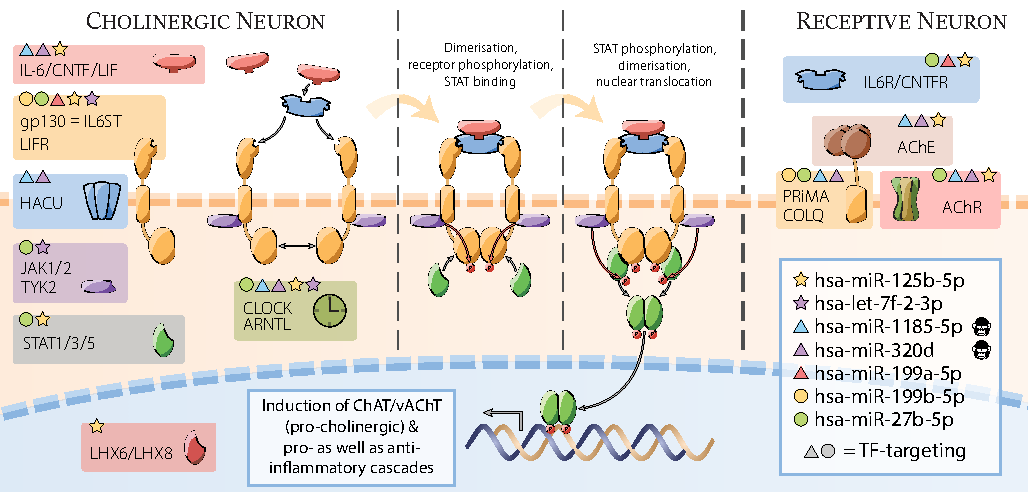
\includegraphics[width=\textwidth]{figures/neurokine}
\caption[The Neurokine Pathway.]{\textbf{The Neurokine Pathway.} The neurokines, such as CNTF, LIF, and IL-6, signal through a combination of soluble and membrane-bound receptors. Activation of a transmembrane neurokine receptor is usually followed by JAK recruitment and phosphorylation, and successively by STAT activation and translocation to the nucleus. Gp130-family neurokine, cholinergic, and circadian signalling pathways are controlled by primate-specific and evolutionarily conserved miRNAs. miRNA targeting of individual genes (indicated by coloured symbols) yields complex transcriptional interactions. Several miRNAs directly targeting the cholinergic pathway also target TFs controlling this pathway (circles and triangles).
\label{fig:neurokine}}
\end{figure}

%Neuronal activity is profoundly modified by cytokines

%Oleg Butovsky - TGFbeta as master glia regulator


%!TEX root = ../dissertation.tex
\newpage

\section{Transcriptional Connectomics}
The term »connectomics« is not strictly limited to one scientific discipline; it is frequently used when the studied matter is defined by complex relationships between interaction partners. The most frequent use outside of transcriptional matters is neuronal connectomics, i.e., the relationships and projections between brain regions. In this dissertation, connectomics generally refers to epi\-/transcriptional interaction, the processes surrounding protein-coding gene expression. For the sake of simplicity, in this dissertation all observations relating to genomics, transcriptomics, genes, and their small RNA regulators should be seen in the context of \textit{Homo sapiens}, unless explicitly stated otherwise.

\newthought{No matter their location}, cholinergic neurons are defined by their ability to synthesise \ac{ach} and release it to neighbouring cells to a certain effect. To fulfil this task, two particular proteins are essential: the \acf{chatp} to synthesise \ac{ach} from choline and acetyl-Coenzyme A, and the vesicular acetylcholine transporter (\acs{vacht}, official gene symbol \acs{slc}), which concentrates \ac{ach} in vesicles for later release. A notable genetic feature connects these two proteins beyond their functional association: the small \textit{\ac{slc}} gene - only 2420 \acp{nt} in size - sits inside the first intron of the \ac{chat} gene and thus is already included in its primary transcript, and is subject to the \ac{chat} promoter. However, oftentimes the (mature) transcript levels of \ac{chat} and \ac{slc} mRNA seem to be independently regulated; from the perspective of the organism, the possibility of differential regulation between these two genes makes sense. Since \ac{slc} apparently does not possess its own promoter, this differential regulation has to be conveyed epigenetically. 

This dissertation deals in large parts with approaches aiming to decipher these interactions; and while its primary topic revolves around cholinergic systems, the methods described in the following are designed to be applicable to the entirety of the genome/epigenome. Four particular types of cellular actors are subjects of these methods and therefore will be briefly introduced: genes in the classical sense as the conveyors of cellular function by encoding for proteins; \acp{tf}, a subclass of protein coding genes that are able to regulate the expression of other genes; \acp{mir}, a class of \ac{smrna} that has been known for approximately two decades and is reasonably well described functionally and mechanistically; and \acp{trf}, a second class of regulatory \ac{smrna} that has only recently been rediscovered and is significantly less well described regarding its functionality.

Naturally, there are multiple additional epigenetic regulatory mechanisms that are not subject to the herein described methods, some of which closely interact with small RNA function. For instance, long non-coding RNAs are a large, novel class of RNA that is poorly characterised as of yet, but has been shown in several instances to interfere with gene expression via RNA-binding protein interactions, or with \ac{mir} function via sponging of miRNA molecules. Other epigenetic processes such as DNA methylation or histone modifications are also known to significantly influence gene expression; however, their effects are in most cases not catalogued in a comprehensive fashion and thus are not amenable to whole-genome bioinformatics analyses.

\subsection{Transcription Factors} \label{sec:intro:tf}
\Acfp{tf} were among the first intracellular regulatory mechanisms to be discovered (the earliest article referencing the term »transcription factor« in its title on PubMed was published in 1972). \acp{tf} commonly translocate from the cytosol into the nucleus upon activation (often by phosphorylation), where they bind specific DNA sequences that usually range in size from 6 to 12 \acp{nt}. The regions containing these binding sites (about 100 - 1000 \ac{nt} in size) determine the effect upon binding, which can be one of two main modes: either a promoter, leading to an increased activity of transcription in the downstream vicinity of the binding site, or a repressor, having the opposite effect. 

There exists a vast body of knowledge on \ac{tf}-interactions with genes, mostly due to the long period of time since their discovery and the multitude of scientific publications, most often studying single \acp{tf} and their interactions with few genes, but cumulatively curated by several organisations. One of the currently largest curations of \ac{tf} data, TRANSFAC, saw its original release in 1988. While these curation efforts can be extensive, they may present with serious bias towards particular \acp{tf} that may hold more scientific interest and thus are published far more frequently than others. Recently, comprehensive efforts have extended the available data significantly. Driven by the advent of \ac{seq}, computational approaches have become able to not only comprehensively predict \ac{tf}-gene interactions, but to do so in a highly tissue-specific manner (see Section \ref{sec:database:tf}). The human body is estimated to express up to 2600 distinct DNA-binding proteins, most of them presumed \acp{tf},\cite{Babu2004} although other studies give lower estimates. 

\subsection{microRNAs} \label{sec:intro:mirna}
The first endogenous »small RNA with antisense complementarity« was described in 1993,\cite{Lee1993} but \acfp{mir} were only recognised as a distinct regulatory class of molecules in the early 2000s. They are typically between 18 and 22 \ac{nt}-long, single stranded RNA fragments, and their function is now largely undisputed: \acp{mir} serve as targeting molecules for a protein complex whose primary purpose is to repress translation of mRNA, and, in some cases, lead to mRNA degradation. The complex, therefore, is called \ac{risc}; central to its function is the family of \ac{ago} proteins, which can bind the mature \ac{mir} and orient it for interaction with its targets (Figure \ref{fig:schirle2014}).\cite{Elkayam2012} Guidance of \ac{risc} to the target mRNA is generally mediated via sequence complementarity between \ac{mir} and the targeted mRNA. Specifically, a »seed« region, usually bases 2-8 on the \ac{mir}, is mainly responsible for the interaction; in case of perfect complementarity of this seed to the mRNA sequence, the interaction is considered »canonical«.\cite{Schirle2014}

\begin{figure}
\includegraphics[width=\textwidth]{figures/schirle2014}
\caption[Structure of the Ago2-guide complex.]{\textbf{Structure of the Ago2-guide complex.} \textbf{A)} Schematic of the Ago2 primary sequence. Front and top views of human Ago2 bound to a defined guide RNA (red). Ago2 contains a large central cleft between two lobes (N-PAZ and MID-PIWI) connected by two linker domains (L1 and L2). \textbf{B)} Guide RNA omit map contoured at 2$\upsigma$ (blue mesh). \textbf{C)} Nucleotides g2–g5 are exposed, whereas Ago2 occludes nucleotides g6 and g7. \textbf{D)} The 3' half of the guide is threaded through the N-PAZ channel. \textbf{E)} View down the N-PAZ channel. Figure and caption from Schirle \emph{et al.}\cite{Schirle2014}
\label{fig:schirle2014}}
\end{figure}

In early \ac{mir} research, the 3' \ac{utr} of the mRNA was believed to contain most \ac{mir} binding sites due to its greater accessibility (i.e., the lack of active ribosomes); however, cumulative recent reports suggest that binding inside the coding region of the mRNA is a regular occurrence.\cite{Hausser2013} The rules governing \ac{mir} binding to target sequences show considerable flexibility; a recent study shows about 30\% of analysed relationships to be of »non-canonical« nature.\cite{VanPeer2018} In those cases, seed pairing with the mRNA is often imperfect. To ameliorate this loss of stability, compensation occurs typically by a secondary complementary structure after a small gap of non-complementary bases, leading to a »bridge«-type constellation (Figure \ref{fig:vanpeer2018-mirna-binding}). This flexibility has implications in applications involving targeting algorithms; those that consider only the seed region are more prone to false negatives than models that consider, for instance, the free energy of the whole molecule (see Section \ref{sec:database:mirna}). A recent study reveals a highly unusual non-canonical binding of miR-126-3p directly to caspase 3, inhibiting apoptosis independent of RISC association.\cite{Santovito2020}

\begin{figure}
\includegraphics[width=\textwidth]{figures/vanpeer2018-mirna-binding}
\caption[miRNA Binding Modes.]{\textbf{miRNA Binding Modes.} miRNAs can bind to their target transcripts via a range of binding modes. N: any nucleotide; M: matching nucleotide. \textbf{A)} Simple seed matching of complementary bases (indicated by grey lines) is called canonical binding. Canonical sites can have different lengths and starting points. \textbf{B)} Seed pairing can be supplemented by complementarity in the 3' region of the miRNA, often after a »bridge« of non-complementary bases. This is particularly relevant in case of a mismatch in the seed (indicated by red »X«). Possible but less frequent are also \textbf{C)} offset 6-mer sites, \textbf{D)} seed-mismatched or G:U wobble sites, and \textbf{E)} G-bulge sites. Figure modified from van Peer \emph{et al.}\cite{VanPeer2018}
\label{fig:vanpeer2018-mirna-binding}}
\end{figure}

\subsubsection{Biogenesis}
\acp{mir}, similar to coding genes, are transcribed from loci on the genome, many inside introns or even exons of coding genes.\cite{Rodriguez2004} The primary transcript (primary \ac{mir} or pri-\ac{mir}) typically contains a hairpin-like structure that usually results in a double-stranded molecule because of internal complementarity, and can contain up to six mature \acp{mir}. This hairpin structure is recognised by the DGCR8 protein (DiGeorge Syndrome Critical Region 8, in invertebrates called »Pasha«); the complex then associates with the RNA-cleaving protein »Drosha«, which removes bases on the opposite side of the hairpin, creating a \ac{mir} precursor (or pre-\ac{mir}), which is subsequently exported from the nucleus by the shuttle protein Exportin-5. In a final step in the cytosol, the ribonuclease »Dicer« removes the loop joining the 3' and 5' arms of the pre-\ac{mir}, resulting in a duplex of mature \ac{mir}, about 20 \acp{nt} long. Initially, it was thought to contain only one active \ac{mir}, resulting in a designation of »\ac{mir}*« for the complementary strand (commonly, the strand with lower expression). However, this notion has been disproven, and to reflect the possibility of both strands performing \ac{mir} functions, nomenclature has changed to specify the arm of the pre-\ac{mir} from which the mature form originates (suffix »-3p« for the 3' arm, and »-5p« for the 5' arm).

\ac{mir} genes, in the same way as protein coding genes, can be subject to promoters and repressors, adding another layer of expression control by \acp{tf}. However, these \ac{tf}-\ac{mir} relationships are far less well described than common coding gene interactions, because \acp{mir} due to their shortness are not amenable to many standard gene expression assay forms. Estimation of the number of distinct gene targets of any one \ac{mir} varies widely; however, it is generally accepted to not be less than several dozen targets per \ac{mir}, and up to thousands of genes per \ac{mir} (although that estimate may be overenthusiastic).\cite{Hendrickson2009, Zhdanov2009}

\subsubsection{Organisation and Curation}
\acp{mir} are organised and curated by means of a periodically updated web-based platform, miRBase.\cite{Kozomara2019} For \textit{Homo sapiens}, miRBase v21 contains 2588 mature \acp{mir} from 1881 precursors. Evolutionarily, the \ac{mir} repertoire has grown from rodents to primates, resulting in a number of primate-specific \acp{mir} that may convey additional function. \ac{mir} nomenclature is organised\cite{Ambros2003} in a way that assigns evolutionarily conserved \acp{mir} the same designation (number) in all species in which they are expressed. In their full names, a prefix stating the organism of origin is added; for example, hsa-miR-125b-5p (for \textit{Homo sapiens}) and mmu-miR-125b-5p (for \textit{Mus musculus}) share the same sequence and most of their functionalities.

\acp{mir} are subcategorised in families (designated »mir« with lowercase »r«) by their genomic origin and phylogenetic homology aspects. As the annotation itself, family affiliations are in flux and change with each miRBase version. miRBase v21 lists 151 distinct \ac{mir} families with 721 individual members in total. The remaining 1867 \acp{mir} do not (yet) belong to a larger family; the majority (80\%) of those is newly discovered, as indicated by a 4-digit designation number.

\subsubsection{Disease Association}
\acp{mir} have been associated with a number of \ac{cns} diseases, including \ac{ad}, \ac{pd}, \ac{bd}, and \ac{scz}. However, the largest contribution since their discovery by far has been made by cancer research; of the approximately \num{90000} publications found on PubMed with the term \ac{mir}, about \num{42000} involve cancer (search term »\ac{mir} AND cancer«). In comparison, »\ac{mir} AND Alzheimer's Disease« results in about 600 hits, while a search for »\ac{mir} AND Schizophrenia« yields just 363 publications (as of October 2019).

In \ac{ad}, several groups of \acp{mir} have been found to show characteristic perturbations before the onset of symptoms, which makes them interesting biomarker candidates.\cite{Salta2017a} Some \acp{mir} have been extensively studied in a variety of contexts, most prominently hsa-miR-132-3p. Among its targets are several key neuronal regulators (e.g. FOXP2, FOXO3, P300, MeCP2), and it is in turn controlled by many pivotal neuronal elements (e.g. REST, ERK1/2, CREB); this presents an explanation for the many physiological and pathological situations that miR-132-3p has been found to play a role in. Its functions include the control of neuronal survival/apoptosis, migration and neurite extension, neuronal differentiation, and synaptic plasticity. 

\acp{mir} fulfil their regulatory purpose in a context- and cell-type-dependent manner,\cite{Lu2015} such that the perturbation of one single \ac{mir} may provide different functional outcomes in different tissues (e.g., glial cells and neurons), or different stages of disease. However, this »jack-of-all-trades« behaviour also poses significant problems in establishing \acp{mir} as pharmacological targets: In the case of antagonising or mimicking an existing \ac{mir}, the amount of off-target effects would not only be enormous, the entire definition of an off-target effect would continuously change between tissues and during the course of the disease. For this reason, the design of custom oligonucleotides with limited capabilities may be preferable in the development of therapeutics based on RNA interference (See also Section \ref{sec:discussion:therapy}).

\subsection{Transfer RNA Fragments} \label{sec:intro:trfs}
\Ac{trna} breakdown products have been known for decades, with first descriptions in the 1970s; back then, they were associated with a higher turnover of \ac{trna} in cancer cells,\cite{Borek1977} and proposed as urine-based biomarkers for certain malignancies.\cite{Speer1979} However, their genesis was attributed to random processes, and due to lacking molecular biology characterisation techniques, interest in those fragments quickly faded. It was not until recently that studies have shown \ac{trna} to be a major source of stable expression of small noncoding RNA\cite{Cole2009,Lee2009} in most mammalian tissues. Indeed, replicating the reports from the 1970s, but now in the form of comprehensive small RNA analysis of human biofluids,\cite{Godoy2018} \ac{trna} breakdown products are the dominant form of small RNA in secreted fluids, such as urine and bile, and make up large parts of the RNA profile of other bodily fluids as well. They exist in two major forms: \acp{tirna} and the smaller \acfp{trf}. \acp{tirna} derive from either end of the \ac{trna}, and are created by angiogenin cleavage at the anticodon loop.\cite{Yamasaki2009,Ivanov2011} Smaller fragments are derived from the 3’ and 5’ ends of the \ac{trna} (3'-\ac{trf}/5'-\ac{trf}) or internal \ac{trna} parts (i-\ac{trf}), respectively, and may incorporate into \ac{ago} protein complexes and act like \acp{mir} to suppress their targets.\cite{Burroughs2011,Kumar2014}

However, there is considerable controversy about the generalisation of \ac{trf} functions, as distinct publications discover very different and sometimes opposing mechanisms of action for their respective fragments. An obvious assumption is the \ac{mir}-like functionality, at least for those \acp{trf} that are in the length range of \acp{mir}. There have been several instances of \acp{trf} proven to act as \ac{mir}-like suppressors of translation in a \ac{risc}-associated manner,\cite{Kumar2014} and of Dicer playing a large part in their biogenesis.\cite{Cole2009} There are even instances of small RNA molecules previously mislabeled \acp{mir} that have been discovered to actually be \ac{trna}-derived, such as miR-1280.\cite{Huang2017}

On the other hand, multiple groups have identified \acp{trf} to function not in an antisense\-/complementary manner, but by homology aspects. A valine-derived \ac{trf} was found to regulate translation by competing with mRNA directly at the binding site at the initiation complex and thereby displacing the original mRNA, leading to its translational repression.\cite{Gebetsberger2017} Others have found multiple classes of \acp{trf} derived from glutamine, aspartate, glycine, and tyrosine \acp{trna}, that displace multiple oncogenic transcripts from an RNA-binding protein (YBX1), conveying tumour-suppressive activity.\cite{Goodarzi2015} Most counterintuitive is the recent finding of a \ac{trf} proven to bind to several ribosomal protein mRNAs and \emph{enhancing} their translation, and, when specifically inhibited, leading to apoptosis in rapidly dividing cells.\cite{Kim2017}

There is no consistent nomenclature yet to describe and organise \acp{trf}, which are by nature more heterogeneous than \acp{mir}; while only 61 mature \acp{trna} are required in a cell to achieve a one\-/to\-/one »codon$\to$amino acid« translation, one \ac{trna} molecule can be the origin of several hundred distinct \ac{trf} molecules. Additionally, the amount of human \ac{trna} genes is estimated at 500-600,\cite{Parisien2013} and there are many more pseudo-\ac{trna} genes. To communicate the identity of individual \acp{trf}, multiple approaches are common in current literature; most prominently, \acp{trf} are tied to the parent \ac{trna} and the amino acid carried by this \ac{trna}. To illustrate: The 22-nt LeuCAG3′ \ac{trf} (meaning: a fragment of 22 bases starting at the 3' end of the leucine-carrying \ac{trna} with anticodon »CAG«) was shown to play an important role in regulating ribosome biogenesis.\cite{Kim2017} Since there is no repository of the likes of miRBase yet, this approach can be cumbersome for replication purposes, and explicit statement of the exact sequence of each fragment is a must in publication. In fact, since the aforementioned paper does not mention the sequence explicitly, there exist six distinct possibilities of fragments fitting this description. While manageable on this small scale, this system prohibits efficient analysis of larger sets of \acp{trf} that cannot be individually controlled. For this reason, the approach of Loher and colleagues\cite{Loher2017} may be preferable: they propose the generation of a »license plate« based on the sequence of the fragment directly, composed of the prefix »\ac{trf}«, the length of the fragment, and a custom oligonucleotide string encoding (e.g., »B3« codes for »AAAGT«). This way, \ac{trf} names are unique and unmistakably linked to the sequence, nomenclature is species-independent, and \ac{trna} origin can be quickly determined by sequence lookup.

%Levels of \acp{trf} may be modulated even more rapidly than levels of \acp{mir}, since \ac{trna} molecules are very abundant in the cell and generation of mature \acp{trf} requires only enzymatic degradation of \ac{trna} but no de-novo transcription of the molecule in the nucleus (citation).

\section[Nested Multimodal Transcriptional Interactions - The Need for Connectomics]{\nopagebreak{Nested Multimodal Transcriptional Interactions\\ \qquad \qquad - The Need for Connectomics}}
The ultimate aim of transcriptional connectomics is the combination of all interacting cellular components in a model that satisfactorily explains our real-life observations and is able to predict the functional outcome of a modification of one of these players. Even in the simplified case of only studying the interactions between coding genes, \acp{tf}, \acp{mir}, and \acp{trf}, the complexity of the required model exceeds our current capabilities by far. The more we know about the functioning of these intertwined systems, the more we understand how much there is still to learn. 

For instance, only recently has it become clear how complex transcriptional regulation by means of \acp{tf} really is, and, incidentally, the two systems studied foremost in this dissertation (nerve and immune cells) are the two most transcriptionally complex systems in any mammal.\cite{Marbach2016} Through study of comprehensive genomic information of 394 tissue types in approximately 1000 human primary cell, tissue, and culture samples (from the FANTOM5 consortium) it was estimated that the mean number of active \acp{tf} towards any given gene is highest in immune (12 \acp{tf} per gene) and nervous cells (10 \acp{tf} per gene), and that any one \ac{tf} in nervous and immune cells controls expression of a mean of 175 and 160 genes, respectively (see also Section \ref{sec:database:tf}).\cite{Marbach2016}

Similarly, it has been found that \acp{mir}, particularly in the nervous system, possess a much higher tissue specificity than coding genes, resulting in an expression landscape that varies widely between individual neuron types that are in close proximity in the brain. With the exception of single cell \ac{seq}, no modern analysis method is capable of a resolution appropriate for accurate characterisation of these expression patterns, resulting in extinction of the signal of \acp{mir} that are not expressed consistently across cell types (similar to »housekeeping« genes) because of statistical interference. Very recent studies show that \ac{mir}:gene co-expression networks are tightly linked to cell types in the nervous system, and that groups of miRNAs as functional modules associate with particular phenotypes in developmental and mature states.\cite{Nowakowski2018} This functional association with cell phenotype was found in quality comparable to the expression patterns of \acp{tf}, yet in quantity conveys smaller impact and thus is thought to be a fine-tuning mechanism, subtle and precise in purpose. 

Another aspect of the tissue specificity of \ac{cns}-associated \acp{mir} is the high likelihood of under-representation or even non-discovery of those very specifically expressed \acp{mir}. Adding to the problem is the experimental bias towards rodent models when it comes to thorough studies of the \ac{cns}, where human or other primate samples are a rarity compared to rats or mice. Assessments of the numbers of yet unknown novel primate- and tissue specific \acp{mir} estimate their magnitude in the thousands,\cite{Londin2015} resulting in an effective doubling of currently known \acp{mir}.

These high numbers of potentially interacting players present computational challenges: Approximating the number of expressed genes in a human cell at \num{20000}, the number of \acp{tf} at a low 500, and an actual number of interactions per TF at 10, the total possible interactions $C$ are given by $$ C = \frac{500!}{10!(500-10)!} \cdot \num{20000} $$ which practically equals infinity. This is without accounting for different tissue types or cell states (e.g., differentiation or disease). Similarly, the amount of mature \acp{mir} (2588 in miRBase v21) and their ability to target even more distinct transcripts than \acp{tf} with one single molecule present immense computational requirements for even listing all possible or actual relationships. An interaction table describing targeting of genes by \acp{mir} in one type of tissue has $ 2588 \cdot \num{20000} \approx 50$ million individual fields.

Combining the different modes of transcriptional interaction presents additional challenges. A simple model system to visualise (in only one type of cell) the interaction of \acp{tf} targeting genes, and of \acp{mir} targeting genes as well as \acp{tf}, contains about \num{20000} genes (a subset of which of the size of about 2000 are \acp{tf}), 2588 mature \acp{mir}, and a total of $ 2588 \cdot \num{20000} + 2000 \cdot \num{20000} \approx \num{90000000} $ potential interactions. In standard application scenarios, such as the generation of an interaction network around a group of genes (e.g., the cholinergic genes), the processing requirements grow linearly with each added interaction partner, and exponentially with every regulatory layer that is added.

Practically, this information has to be provided, gathered, and integrated, which further multiplies the amount of storage and processing power required. miRWalk 2.0, a collection of \ac{mir} interaction data, has collected 12 of the most popular \ac{mir}-targeting prediction datasets, each of which has their strengths and weaknesses (see \ref{sec:database:mirna}). Experimentally validated interactions (e.g. as collected in DIANA TarBase or miRTarBase) are gold standard, but far from comprehensive and strictly speaking only relevant for the cellular context in which the experiment was originally performed; there are also different evidence qualities to be accounted for, depending on the type of experiment performed. Ideally, all of these data are still accessible when performing the analysis, so a database created for this purpose should be able to incorporate all this information without any data loss while still remaining feasible in terms of computation time as well as space and working memory requirements. 

This dissertation will first describe the creation of such a database and what has been learned during its various stages, and then go on to apply the database to different biological problems from real world experiments, such as the cholinergic differentiation of human male and female cultured neuronal cells, and the blood of stroke victims.


%!TEX root = ../dissertation.tex
\begin{savequote}[75mm]
»Wir sehen in der Natur nie etwas als Einzelheit, sondern wir sehen alles in Verbindung mit etwas anderem, das vor ihm, neben ihm, hinter ihm, unter ihm und über ihm sich befindet.«
\qauthor{Johann Wolfgang von Goethe}
\end{savequote}

\chapter[miRNet: Creation of a Comprehensive Connectomics Database]{\textit{miRNet}: Creation of a\\Comprehensive Connectomics Database} \label{sec:database:mirnet}
Natural philosophy, as represented by the thought of Johann Wolfgang von Goethe, is concerned with the holistic description of nature and the explanation and interpretation of its particular mechanisms. Although natural philosophy is the predecessor of modern, empirical science, its concepts and approaches are still valuable in today's data driven world; as the data we collect grows to dimensions that can only be interpreted computationally, functional reductionism becomes all the more important: By studying the facets of nature, we strive to understand it as a whole. Similarly, we regularly encounter Goethe's paraphrase of »all things are connected« in transcriptional connectomics.

\newthought{Bioinformatic support in connectomics} is indispensable, which can be seen by the sheer multitude of possible interactions between the participating factors. However, when I began working on this project (October 2015), there was no integrative database available for this purpose. Earlier that year, miRWalk 2.0 had been published, for the first time providing a relatively comprehensive source of predicted as well as experimentally validated \ac{mir} targeting data\cite{Dweep2015} (see \ref{sec:intro:mirna}). One year later, Marbach's »regulatory circuits« were published\cite{Marbach2016}, enabling analysis of comprehensive \ac{tf}$\to$gene relationships in 394 human tissues (see Section \ref{sec:intro:tf}). These collections (as well as the data they were derived from) are the basis of the database further called \textit{miRNet}, the development of which will be described in the following chapter.

Since a large part of the scientific progress of this dissertation deals with practical problems of multimodal connectomics, I will begin by describing the infrastructure that makes effective computation of these problems possible. After this technical description of database structure and creation, I will explain the types and organisation of its content. The remainder of the chapter will then deal with the application of this infrastructure to real-world problems in transcriptional connectomics, and the statistical approaches suited to this special case.

\section{Implementation}
For any biological question to be asked in a bioinformatics setting, the effectiveness of the computational query determines the practicality of the approach. Because resources (i.e., processing power, storage, and working memory) are limited, the database that is queried should be organised in a way that facilitates retrieval of the desired information without excess processing of useless information. In the simplified case of only \acp{mir} interacting with genes in one direction (\ac{mir}$\to$gene), this means retrieval of only those interactions relevant for the queried genes or \acp{mir}. 

Traditional table-based approaches (also known as relational databases) such as \acs{sql}  (»Structured Query Language«) cannot provide such an implementation, since individual entries for genes and \acp{mir} (rows and columns) have to be accessed in their entirety, whether there is a connection between gene and \ac{mir} (1) or not (0). Additionally, adding layers to these interactions (e.g., distinct prediction algorithms, tissues, or the interaction between \acp{tf} and genes) require the addition of entire tables the same size as the database, which is detrimental to effective use of space; and more complex queries also necessitate the transfer of information between those distinct tables (in \ac{sql} typically via a \textcolor{dkblue}{JOIN} command), which claims additional working memory and processing time. Overall, the so-called »many-to-many« organisation of data does not lend itself to representation in a relational database. 

\todo{Figure to explain tables?}

The actual performance is determined by the processing power of the machine it is running on and several structural properties, such as organisation, indexing, monotony, and of course the size of the database; therefore, an estimation of processing time for queries is bound to be inaccurate. However, processing times typically do not vary on the scale of orders of magnitude, and thus general estimations can be made. Well optimised \ac{sql} databases with a size of 5 to 10 GB on disk usually require tens of minutes if not hours to complete one single complex query\cite{Chaudhuri2004}; \textit{miRNet} in its current form takes up approximately 15 GB of storage. Since one analysis typically consists of several hundreds (and, in the case of permutation analyses, several hundreds of thousands) of these queries, processing times in \ac{sql} implementation are too long to be practically useful. (It seems important to note that, as of 2018, \ac{sql} also offers a graph-based organisation in addition to the traditional, relational layout. These two are separate systems, and not to be confused. The advantages of Neo4j as explained in the following should be seen from the perspective of 2015, when the database was established, and when there was no graph-based \ac{sql} implementation.)

\subsection{Neo4j: A Graph-Based Infrastructure}
To query and display biological data that are organised in a network-like structure (many-to-many), a database that lends itself to the efficient processing and storage of network data is optimal. »Neo4j« utilises a database structure that is built on the save and recall of data points in \emph{nodes} and \emph{edges}, which represent entities (nodes) and relationships between those entities (edges); both nodes and edges can have any number of attributes and a unique property called »type«, usually describing the class of the entry (such as \emph{gene} or \emph{miRNA}). This database organisation replicates the network-like structure of the biological data studied (Fig.\,\ref{fig:graph-org}). Neo4j combines the network-like data structure with an efficient indexing system for quickly finding the entries queried for, and then »walks« along the edges of the nodes that have been found, thus only searching and returning the data that is relevant to the current query. Theoretically, this makes the database more likely to be efficient in the setting of transcriptional interactions, an estimation that turned out to be true.

\begin{figure}
\includegraphics[width=\textwidth]{figures/graph-org}
\caption[Graph database organisation.]{\textbf{Organisation of a graph database.} A graph consists of two basic building blocks: \textit{Nodes}, representing entities, and \textit{edges}, representing connections between entities. Each database entry (node or edge) is an instance of a particular \textit{type} and can possess an arbitrary amount of \textit{properties} detailing its specifics.
\label{fig:graph-org}}
\end{figure}

Depending on the input, these queries can also be rather large; however, the main pitfall of tabular databases such as \ac{sql} is circumvented: there is no need to process entire rows or columns of the table to make sure that the query is satisfied in its entirety. This is particularly useful in a setting of sparse information. To illustrate: Only 30 of the 2588 \acp{mir} target a specific gene, which is common; a relational database, after finding the index of the queried gene, would have to search 2588 fields for $1/0$. The graph database, on the other hand, has to execute only 30 searches (or, more accurately, 30 »walks« along the edges connected to the indexed node). In practice, even in the very first prototype implementations, this accelerated standard-case computations immensely, and was even able to accommodate advanced approaches in situations that had been inaccessible in the tabular implementation.

\subsection{High-throughput Database Generation}
Neo4j provides several \acs{api} (»application programming interface«) possibilities in implementation. For the purpose of entering large amounts of data into the database at once, the Java implementation is superior to the other forms in that it provides a batch processing mode via its \texttt{BatchInserter} class. I thus wrote a custom Java program for the purpose of creating an initial state of the database from the largest set of data, the complete miRWalk 2.0 content with 12 algorithms and validated interactions. The downloaded data was organised in a plain text based file format, with one text file for each \ac{mir}, totalling in size about 6 GB (for \textit{H. sapiens}). The database was set up in a way that allows only one node for each individual \ac{mir} and gene entered to avoid duplications, using the commands 
\begin{itemize}[noitemsep, leftmargin=.5cm, label={\tiny\raisebox{1ex}{\textbullet}}]
\item \texttt{createDeferredConstraint()}
\item \texttt{assertPropertyIsUnique()}
\item \texttt{createDeferredSchemaIndex()} 
\end{itemize}
of the Neo4j Java package. This approach made sure to create only one node for each \ac{mir} (type: MIR) and gene (type: GENE) in the data, which is essential for proper functioning of the database. Each of these nodes received several properties to store individual data, such as the various gene/\ac{mir} identifiers, miRNA sequence, and species. 

Between those basic nodes, the batch insertion process created edges for each relationship that was found in the original data, assigning a type identifier to each edge detailing the origin of this interaction (type: name of the prediction algorithm or »VALIDATED« for experimental data). Thus, while the nodes for genes and \acp{mir} themselves are unique, an arbitrary number of relationships can exist between any two nodes, depending on how many interactions they share.

\subsection{Maintenance and Quality Control}
All additional datasets, such as the \ac{tf} regulatory circuits or \ac{trf} targeting predictions, were entered into \textit{miRNet} using the regular operation mode. Testing was also performed in regular operation, with manual as well as automated tests to assert the correct transfer of information from raw data to the graph database, and to avoid unpredictable behaviour. At times, conflicts had to be resolved manually, for instance when \ac{mir} names conflicted between old »\ac{mir}*« and new »3p/5p« notation; all manual edits are documented in the code, which was published alongside Lobentanzer et al\cite{Lobentanzer2019a}.

Except for the rapid import of large amounts of data in creation of a database, the Java implementation of Neo4j does not offer many advantages over the native R implementation, »RNeo4j«. Thus, after creation and a short period of experimentation with graphical user interfaces, I abandoned the Java program in favour of the more flexible R programming. While Java is an object-based programming language, whose benefits lie in extreme flexibility in regards to platform and purpose, high modularity, and speedy processing, R as a procedural language is the work horse of modern bioinformatics. Its procedural design (the division of data and functions that operate on that data) facilitates the transfer of approaches between distinct datasets, and the enormous vibrant community of data scientists using R provides a wealth of third party packages to tackle almost any bioinformatic task. In the remainder of this dissertation, all analyses are performed in R, unless specifically stated otherwise.

\section{Materials}
All materials used in the creation of \textit{miRNet} have been acquired from resources that are non\-/commercial, web-available, and open-source (in the case of code). All properties and relationships derived from this data were entered into \textit{miRNet} as either nodes, properties of nodes, edges, or properties of edges. 

\subsection{Gene Annotation}
Even though »regular« protein coding genes have been known for a long time, there is no consensus yet about their nomenclature and organisation. Complicated by newly discovered functions and properties of phylogenetic nature, the scientific representation of the human genome is in constant flux. Several large organisations strive to provide a robust annotation of the human gene catalog, but also in many cases contradict one another. There are three nomenclature systems that are of high importance in modern genomics: 
\begin{itemize}[noitemsep, leftmargin=.5cm, label={\tiny\raisebox{1ex}{\textbullet}}]
\item The traditional naming system of acronyms (e.g. \ac{chat}) and fantasy-names (such as »Sonic Hedgehog«), also occasionally called »gene symbol«, is still widely popular because of its accessibility to humans, but is also not particularly robust because of a high amount of synonyms with high confusion potential (see e.g. Section \ref{sec:intro:neurokine} on CDF) and instances of genes without names having to carry unwieldy systematic names.
\item The American (\ac{ncbi}), a branch of the National Institute of Health (NIH), curates and hosts a multitude of biological and medical data, and for the organisation of gene information uses its own systematic nomenclature termed »Entrez« ID. Entrez is a molecular biology database that integrates many aspects of biology and medicine in a gene-centred manner, and therefore Entrez IDs are useful to quickly connect a gene to its function, nucleotide sequence, or associated diseases. Entrez IDs are regular integers without additional characters.
\item Akin to the \ac{ncbi} effort, ENSEMBL is a project of the European Bioinformatics Institute (EBI) as part of the European Molecular Biology Laboratory (EMBL). Compared to the Entrez database, it is more focused on study and maintenance of the genome itself, and therefore has a more intricate nomenclature that allows for differentiation of, for example, genes and their various transcript isoforms (ENSEMBL IDs carry character prefixes for class identification, e.g., ENSG for genes, ENST for transcripts).
\end{itemize}
All of these are being used on a regular basis in many publications, and, often, they are used exclusively. As a result, the end user of the published data has to have access to all possible annotation forms, or, at least, a means to translate one into the other; often, this also introduces conflicts. For this reason, all ID types were entered into \textit{miRNet} upon creation or during maintenance, for convenience and to minimise analysis prolongations due to conflict resolution.

\subsection{microRNA Annotation}
miRBase provides a consistent annotation for \acp{mir}. Due to their relatively recent discovery, there still are major changes from version to version; the syntax, however, is stable. In addition to the \ac{mir} »names« that are composed of species, the string »miR«, pre-\ac{mir} designation number, and strand origin (not in all cases!), such as »hsa-miR-125b-5p«, miRBase provides IDs for pre-\ac{mir} molecules (also called ancestors) termed »MIID«, and IDs for mature \ac{mir} molecules termed »MIMAT«. However, in practice, these are rarely used. Similarly, \ac{mir} families are annotated using the »MIPF« ID.

\subsection{Transcription Factor Targeting} \label{sec:database:tf}
The FANTOM5 project has applied \ac{cage} to a large number of human samples from diverse tissues to determine the accurate 5' ends of each transcript\cite{Hon2017}. Knowledge of this fact enables accurate prediction of promoters likely to control a transcript's expression. Marbach and colleagues used this information in combination with detailed human gene expression data to derive a complex interaction network of \acp{tf} and genes (»regulatory circuits«), and in doing so aggregated samples with similar expression patterns and origins into 394 fictional tissues\cite{Marbach2016}. For every tissue, each \ac{tf} was assigned transcriptional activities towards all genes that it supposedly targets (with the sum of all activities in any given tissue being \num{1}). Marbach and colleagues have shown that the cumulative transcriptional activities towards any given gene correlate well with the actual gene expression in corresponding samples from an independent repository.

Even in its fifth iteration, FANTOM data is not entirely comprehensive, which came to my attention due to a cholinergic anomaly: The 5' \ac{cage} peaks of the \textit{\ac{chat}} and \textit{\acs{a7}} (the nicotinic $\alpha$7 receptor subunit) genes in raw FANTOM5 data do not pass the expression threshold, and therefore are not included in, e.g., Marbach's »regulatory circuits«. Both are critically important not only for neuronal cholinergic systems, but also for the non-neuronal aspect of immune processes. For instance, macrophages have been shown to produce \ac{ach} via \ac{chat}, and the $\alpha$7 homomeric \ac{ach} receptor conveys direct immune suppression by its expression on monocytes\cite{Fujii2017}. Paradoxically, the \ac{cage} peak of \textit{\ac{slc}}, which lies in the first intron of \textit{\ac{chat}}, crosses the threshold and therefore is included in the data. Unfortunately, I was not able to remedy these circumstances even upon personal communication with Daniel Marbach (author of »regulatory circuits«) and Hideya Kawaji of the FANTOM5 consortium, although the latter acknowledged the possibility of a gene annotation deficit leading to misattribution of the \textit{\ac{chat}} signal to \textit{\ac{slc}} due to the closeness of their 5' ends.

The entire collection of transcriptional activities in all tissues was downloaded from the project's web page\cite{Marbach2016}, and neuronal and immune tissues were manually curated and entered into \textit{miRNet}. The collected data comprises 33 neuronal tissues and 26 immune cell tissues (Appendix \ref{appendix:marbach}), and \num{1130196} \ac{tf}$\to$gene relationships in total (not all 394 tissues were entered). 

\subsection{microRNA Interactions} \label{sec:database:mirna}
The content of miRWalk 2.0 is freely available online\cite{miRWalk2}; however, there is no option of downloading the complete set. The targeting data thus was downloaded per \ac{mir} using a custom crawler, with standard options for all 12 prediction algorithms (miRWalk, miRDB, PITA, MicroT4, miRMap, RNA22, miRanda, miRNAMap, RNAhybrid, miRBridge, PICTAR2, and TargetScan) in plain text format. For experimentally validated interactions, the main sources were DIANA TarBase\cite{Karagkouni2018} and miRTarBase\cite{Chou2018}, both of which offer complete download options. As of 2019, the 3.0 version of miRWalk allows complete species downloads; however, the developers have abandoned their third party algorithm plurality reducing the number of available alternatives from 12 to 4, which can be considered a significant disadvantage:

While sequence complementarity, particularly of the »seed«-region, is the primary paradigm of \ac{mir}-mRNA interaction, prediction algorithms vary widely in their implementation, general purpose, and approach to interaction prediction (for a comprehensive review of approaches and rules, see \cite{Yue2009}). A large group of available options utilise sequence conservation aspects to increase candidate viability (such as miRanda, PicTar, TargetScan, and microT4). Others, such as RNA22 and PITA, utilise biophysical aspects such as free energy of binding or the accessibility of target sites due to secondary RNA structures as prediction arguments. All of these approaches have their up- and downsides, e.g. considering their general precision and sensitivity, or their adequate prediction of particular cases, such as multiple site targeting. Thus, it has been proposed to use a combination of complementary approaches instead of only one algorithm per analysis\cite{Witkos2011}. For this reason, I might have preferred the 2.0 version of miRWalk, even if 3.0 had been available at the time.

One advantage of the collection of all data in a quickly accessible database is the opportunity to compare the different approaches to target prediction. A statistical evaluation of the collected interaction data from miRWalk 2.0 showed vast differences in general prediction quantity (Table \ref{tab:alg.hit.freq.all}) as well as prediction accuracy and sensitivity when compared to the validated subset of data (Table \ref{tab:alg.hit.freq.val}). Since the ground truth is not known, this is an additional argument for the combination of multiple algorithms instead of the use of a single set. Apart from RNAhybrid and miRBridge, all algorithms presented reasonable base hit frequencies and increases in the validated test set. While miRBridge already has the lowest positive frequency of all the algorithms, it is the only one to achieve a negative score in the validated test set. On the other hand, RNAhybrid has a vastly higher base hit frequency than the second highest scoring algorithm (by more than \num{300}\%), making it very likely to produce false positive results, and less valuable in the aggregation scoring system. The remaining 10 algorithms were included in \textit{miRNet} targeting data. For ease of use, an additional relationship type was created from the aggregated single algorithm hits of any \ac{mir}$\to$gene relationship, with the sum of algorithms predicting the interaction as a score variable. This yields a theoretical score range from \num{3} to \num{10} (\ac{mir}$\to$gene relationships with only one or two hits were ignored for the sake of space). To account for experimentally validated interactions, each \ac{mir}$\to$gene relationship that was supported by strong evidence of interaction was modified by addition of \num{10.5} score points (a half point for quick identification of a validated relationship), extending the maximum score to \num{20.5} points. The resulting optimised graph contains \num{11687931} human \ac{mir}$\to$gene targeting relationships with a distinct score distribution (Fig.\,\ref{fig:db-score-hist}). In comparison, only 6146 \ac{mir}$\to$gene relationships are experimentally validated with »strong« evidence.

\begin{figure}
\includegraphics[width=\textwidth]{figures/db-score-hist}
\caption[Graph database organisation.]{\textbf{Histogram of \ac{mir}$\to$gene score distribution.} Aggregation of individual algorithms yields a score range of 3 to 10 per individual \ac{mir}$\to$gene interaction. In case of additional existence of experimental validation (evidence level high) for any predicted interaction, score is increased by 10.5. The distribution shows a sharp decrease in predicted interactions towards higher scores, and a maximum of validated interactions at prediction scores 6 and 7. 
\label{fig:db-score-hist}}
\end{figure}

%tables from cholinomir pseudopaper
\begin{table}
\sffamily
\small
%\resizebox{.85\textwidth}{!}{%
\noindent\parbox[t]{.35\linewidth}{
\centering
\begin{tabular}{c | c}
algorithm & hit frequency\\ \hline
\hline
\textcolor{Maroon}{RNAHYBRID} & 71.62\%\\ \hline
\textcolor{OliveGreen}{MIRMAP} & 19.90\%\\ \hline
\textcolor{OliveGreen}{MIRWALK} & 19.74\%\\ \hline
\textcolor{OliveGreen}{TARGETSCAN} & 16.33\%\\ \hline
\textcolor{OliveGreen}{RNA22} & 12.34\%\\ \hline
\textcolor{OliveGreen}{MICROT4} & 11.81\%\\ \hline
\textcolor{OliveGreen}{MIRANDA} & 10.65\%\\ \hline
\textcolor{OliveGreen}{PITA} & 4.90\%\\ \hline
\textcolor{OliveGreen}{MIRDB} & 1.17\%\\ \hline
\textcolor{OliveGreen}{MIRNAMAP} & 0.75\%\\ \hline
\textcolor{OliveGreen}{PICTAR2} & 0.62\%\\ \hline
\textcolor{Maroon}{MIRBRIDGE} & 0.15\%\\ \hline
\end{tabular}
\caption{Prediction algorithms ordered by the fraction of all possible interactions they predict as being real (positive rate). Different algorithms display a wide variation of hit rates in the entirety of predicted interactions between any \ac{mir} and gene. Red: excluded from analysis.}
\label{tab:alg.hit.freq.all}
}
\hfill
\noindent\parbox[t]{.6\linewidth}{
\begin{tabular}{c | c | c}
algorithm & validated hit frequency & hit rate increase\\ \hline
\hline
\textcolor{OliveGreen}{PICTAR2} & 6.98\% & 1129.40\%\\ \hline
\textcolor{OliveGreen}{MIRDB} & 9.80\% & 838.43\%\\ \hline
\textcolor{OliveGreen}{MIRANDA} & 51.73\% & 485.94\%\\ \hline
\textcolor{OliveGreen}{TARGETSCAN} & 70.63\% & 432.51\%\\ \hline
\textcolor{OliveGreen}{MIRNAMAP} & 3.10\% & 410.95\%\\ \hline
\textcolor{OliveGreen}{PITA} & 15.57\% & 317.20\%\\ \hline
\textcolor{OliveGreen}{MICROT4} & 32.60\% & 276.10\%\\ \hline
\textcolor{OliveGreen}{MIRMAP} & 53.86\% & 270.65\%\\ \hline
\textcolor{OliveGreen}{MIRWALK} & 50.95\% & 258.15\%\\ \hline
\textcolor{OliveGreen}{RNA22} & 22.51\% & 182.38\%\\ \hline
\textcolor{Maroon}{RNAHYBRID} & 90.47\% & 126.32\%\\ \hline
\textcolor{Maroon}{MIRBRIDGE} & 0.01\% & 0.00\%\\ \hline
\end{tabular}
\caption{Prediction algorithms ordered by their increase in true positive rate when considering only validated interactions. The hit rate increase when comparing experimentally validated interactions with the entire predicted data (Table \ref{tab:alg.hit.freq.all}) is also subject to strong variation. Hit rate increase is the increase of hit rate if only considering validated data as opposed to all predicted interactions. None of the studied algorithms unite a good precision (hit rate increase) and coverage (validated hit frequency).}
\label{tab:alg.hit.freq.val}
%}
}
\end{table}

\subsection{Filtering of Aggregated Prediction Scores}
For the estimation of the »true« \ac{mir}$\to$gene interactions in the predicted-only data in \textit{miRNet}, two premises are relevant: First, the enormous amount of hits with a score of 3 in all likelihood is an over-estimation, and second, the amount of currently validated interactions can be but a small fraction of »true« interactions. Assuming the truth lies on the axis between these two extremes (i.e., at some score value inside the \textit{miRNet} interactions), the true amount of human \ac{mir}$\to$gene interactions must fall within the range of XX to XX. Looking at the score distribution of all \textit{miRNet} interactions (Fig.\,\ref{fig:db-score-hist}), the maximum amount of validated interactions is predicted by a combination of 6 or 7 algorithms (i.e., a score of 16.5 or 17.5). Thus, to approximate the true state, I chose to apply a low-cut filter to \textit{miRNet} queries at a minimum score of 6. This is the standard case referred to as »\textit{miRNet} query« in the remainder of this dissertation. In some cases, such as the graphical analysis of whole-genome \ac{mir} targeting (see e.g. Section \ref{sec:cellculture:network}), the score threshold was raised to 7 to circumvent computational limitations.

\subsection{De-novo Prediction of tRF Targeting}
Due to the recency of their (re-)discovery, no comprehensive interaction sources exist for transfer RNA fragments. There have been documented cases of \ac{mir}-like behaviours of distinct RNA fragments\cite{Cole2009,Kumar2014}, justifying an attempt to predict interactions in a comprehensive manner. Of the available options for nucleotide interaction prediction algorithms, TargetScan\cite{Friedman2009} seems particularly suited for this task because it provides the option of evaluating the evolutionary conservation of target sites in the putatively targeted genes, thereby providing an additional layer of security: The sequence of 3' \acp{utr} is evolutionarily less stable than the coding part of genes; thus, high conservation of the binding site might indicate evolutionary pressure to keep up the interaction with the fragment, making an actual function of the interaction more likely. TargetScan also presents with reasonable sensitivity and specificity as confirmed by an independent group\cite{Alexiou2009}, and through an additional algorithm allows the attribution of a score based on the branch length (on the species tree) of conserved targeting\cite{Agarwal2015}.

\ac{mir}-like behaviour implies the existence of a region on the \ac{trf} similar to a \ac{mir} »seed«, and TargetScan also expects a seed as input to its targeting algorithm. Since there has been no definitive answer to the question as to where the seed region in \acp{trf} might be, it is safest to assume nothing and explore all possibilities, i.e., simulate every possible seed position for interaction discovery. For this purpose, all discovered sequences of \acp{trf} (exceeding a base mean expression of 10 counts) were chopped into 7-nt pieces (7mers), which is the length of \ac{mir} seeds, and statistically improbable enough to appear in the genome at random; the average length of a human 3' \ac{utr} is 800 \ac{nt}, so the probability of finding any 7mer randomly in any one 3' \ac{utr} is $p = \frac{800}{4^7} = 0.049$, which agrees with the 5\% \ac{fdr} convention.

\todo{Describe Targetscan process}

\subsection{microRNA Primate Specificity}
During the course of evolution, higher organisms typically attained more complexity in a variety of functional categories. The \ac{cns} as the system of highest complexity underwent several drastic developments from invertebrates to lower mammals to higher mammals still. miRNAs are no exception. While many miRNAs are functionally as well as literally conserved in all mammals, primates in particular have gained a substantial amount of novel miRNAs whose function is in large parts elusive. Due to the restrictions on experimentation on higher mammals, particularly primates, many of those miRNAs can only be studied observationally, or by transgenic experiments in rodents. A cholinergic example of a gain-of-function in higher mammalian miRNA regulation is the vesicular acetylcholine transporter, \ac{slc}. As described in Section \ref{sec:database:tf}, the \ac{slc} gene is situated in the first intron of \ac{chat}, and thus is always primarily co-expressed with the latter. However, a primate-specific miRNA, miR-298, targets the 3' UTR of \ac{slc}\cite{Soreq2015}. Thus, the primate neuron has gained a mechanism of independent \ac{slc}/\ac{chat} regulation that the mouse, for example, does not possess. It is easily imagined that such a gain of neuronal flexibility, in many instances, can aid the development of a more effective brain. However, the primate specificity of miRNAs is not yet consensus, and thus not found in annotation databases such as miRBase, even though they list all miRNAs discovered in any species. To get an impression of the amount of possible gain of function, I performed a review of miRNAs expressed in a representative variety of annotated species.

\begin{method}

\subsubsection{Species Selection}
The tested species were selected from miRBase v21. Some of the available species are severely limited in the extent of miRNA annotation, likely because of a research bias. Therefore, only the most well-annotated species were selected. These are (number of annotated primary and mature miRNAs in brackets):
\begin{itemize}[noitemsep, leftmargin=.5cm, label={\tiny\raisebox{1ex}{\textbullet}}]
\item \emph{Homo sapiens} (human; 1881, 2588)
\item \emph{Gorilla gorilla} (gorilla; 352, 357)
\item \emph{Pan troglodytes} (chimp; 655, 587)
\item \emph{Pongo pygmaeus} (orangutan; 642, 660)
\item \emph{Macaca mulatta} (rhesus macaque; 619, 914)
\item \emph{Bos taurus} (cow; 808, 793)
\item \emph{Canis familiaris} (dog; 502, 435)
\item \emph{Mus musculus} (mouse; 1193, 1915)
\item \emph{Rattus norvegicus} (rat; 495, 765)
\end{itemize}
The first four species belong to the hominid group; the first five are primates. It is likely that these collections are not complete, with the degree of completeness depending on the amount of research performed on the species (as demonstrated, e.g., by the difference between mouse and the other non-primates). This places considerable difficulty on asserting primate specificity of miRNA, and in turn on assertion of the effects of evolution on the miRNA regulatory system.

\subsubsection{Single miRNA Inter-Species Homology Computation}
To determine the homology of miRNAs between the studied species, reference genomes were downloaded from the respective sources and analysed phylogenically, using the genomic coordinates provided by miRBase. Sequence homology was determined via dynamic programming using the Smith-Waterman algorithm\cite{Smith1981}. Briefly, this algorithm can be used to determine the similarity of two genomic sequences, based on a scoring system rewarding matches and penalising mismatches. Smith and Waterman extended the original approach by Needleman and Wunsch\cite{Needleman1970}, which is used to compare two complete sequences. Both algorithms rate an alignment by dynamic scoring inside a 2D-matrix, with the sequences to be compared as the x- and y-axes (one letter per cell). By a change in the scoring system, the Smith-Waterman algorithm finds the best local alignments, instead of comparing the two sequences in their entirety. In the case of miRNAs, this behaviour is useful because, between species, there are frequent additions or deletions of single \ac{nt} on both ends of the homologous miRNA. Genomes were procured from the following sources:
\begin{itemize}[noitemsep, leftmargin=.5cm, label={\tiny\raisebox{1ex}{\textbullet}}]
\item \emph{Homo sapiens}: GRCh38 (NCBI)
\item \emph{Gorilla gorilla}: gorGor3 (UCSC)
\item \emph{Pan troglodytes}: panTro4 (UCSC)
\item \emph{Pongo pygmaeus}: PPYG2 (Ensembl)
\item \emph{Macaca mulatta}: rheMac3 (UCSC)
\item \emph{Bos taurus}: bosTau6 (UCSC)
\item \emph{Canis familiaris}: canFam3 (UCSC)
\item \emph{Mus musculus}: mm10 (UCSC)
\item \emph{Rattus norvegicus}: rn5 (UCSC)
\end{itemize}

Using the genome coordinates provided by miRBase, the genomic sequences of miRNAs and pre-miRNAs of each species were determined. Using the Smith-Waterman algorithm, all identified homologs of human miRNAs were subjected to homology scoring, and score results were visualised as a heatmap.

\end{method}

\subsubsection{Inter-Species Distribution of miRNAs}
The inter-species relationships of annotated miRNAs do not follow a simple evolutionary distribution from less complex to more complex organisms, but rather seem to partially result from parallel development (Fig. \ref{fig:species-homo}). 

\begin{figure}
\includegraphics[width=\textwidth]{figures/species-homo}
\caption[microRNA Species Homology.]{\textbf{Homologues of Human microRNAs in Primate- and Non-Primate-Species.} Homology to human miRNAs was determined by Smith-Waterman local alignment for each homologous miRNA of 8 species. Homology scores were visualised on a heatmap, each column represents the homology to human of the miRNAs of the respective species. The heatmap is ordered from bottom to top by the amount of miRNA homologues in primates. The miRNAs at the very bottom are shared by human as well as all four primate species, followed by the miRNAs shared by three primate species, and so on. Ggo: \emph{Gorilla gorilla}, Ppy: \emph{Pongo pygmaeus} (Orangutan), Ptr: \emph{Pan troglodytes} (Chimp), Mmt: \emph{Macaca mulatta} (Rhesus macaque), Bta: \emph{Bos taurus} (Cow), Cfa: \emph{Canis familaris} (Dog), Mmu: \emph{Mus musculus} (Mouse), Rno: \emph{Rattus norvegicus} (Rat).
\label{fig:species-homo}}
\end{figure}

Taking into account the high probability of missing annotations in several species (particularly hominids), it seems prudent to define primate specificity of miRNAs not by presence in primates, but rather by absence of the miRNAs in non-primate species (also excluding miRNAs \emph{only} annotated in human). This approach yields a list of 377 primary and 350 mature putative “primate specific” miRNAs in miRBase v21 (Appendix \ref{appendix:homologues}). Judging from recent analyses\cite{Londin2015}, there probably exist many more. The primate-specificity attribute was entered into \emph{miRNet} as miRNA node property.

\section{miRNet Usage}
Neo4j uses a language (called »Cypher«) akin to \ac{sql}, which utilises keyphrases to issue commands, but combines it with a semi-graphical syntax to account for the graph-based layout of the data. In the following, I will describe its basic usage and the advantages it provides in the matter of transcriptional connectomics. The basic »finder« function (similar to \textcolor{dkblue}{SELECT} in \ac{sql}) is called \textcolor{dkblue}{MATCH} in Cypher, and, when combined with the semi-graphical syntax, can be used to identify nodes or more complex patterns in the database. The graphical syntax consists of two main building blocks that represent the basic types of data inside the database: nodes as regular brackets »\texttt{( )}« and edges between nodes as  a construct of hyphens and box brackets, that can also have a direction indicated by the greater sign \mbox{»\texttt{( )-\string[ \string]->( )}«}. To specify the elements to be found, attributes of nodes and/or edges can be filtered by using curly brackets in the node definition, or the \textcolor{dkblue}{WHERE} clause. To be returned, elements need to be assigned arbitrary variable names:

\begin{lstlisting}[label=lst:match, caption=MATCH, language=Cypher]
MATCH (gene:GENE {species: 'HSA'})
WHERE gene.name = 'CHAT'
RETURN gene
\end{lstlisting}

Query \ref{lst:match} identifies a node (arbitrarily designated »gene«) with type GENE (indicated by the colon), with attributes »species« (HSA, i.e. \textit{H. sapiens}) and »name« (\ac{chat}), and returns the node with all its attributes. Since the nodes of type GENE are restrained, there can only be one gene of species \textit{H. sapiens} with this name in the database, and thus, only one data point will be returned. The graphical syntax further allows for pattern matching of, for instance, \ac{mir}$\to$gene relationships:

\begin{lstlisting}[label=lst:pattern,caption=Patterns,
language=Cypher]
MATCH (mir:MIR)-[rel:TARGETS]->(gene:GENE {species: 'HSA'})
WHERE gene.name = 'CHAT'
RETURN mir, rel, gene
\end{lstlisting}

Query \ref{lst:pattern}, similar to query \ref{lst:match}, starts by identifying the node of species HSA with the name \ac{chat}, and proceeds to look for \ac{mir}$\to$gene relationship edges arriving at this node; the relationships have to be of the type TARGETS (the pre-aggregated score-based accumulation of targeting). As soon as no further edges are found, the process terminates and returns all found \acp{mir} (»mir«), relationships (»rel«), and genes (»gene«) in discrete form, including all their attributes, such as the ENSG and Entrez IDs, the MIMAT IDs for all found \acp{mir}, or the score value of their targeting relationship. In this query, since there is a constraint on genes, the only gene returned is \textit{\ac{chat}}. However, Cypher is not limited to filtering on unique attributes; it allows for query and return of as many data points as are needed. For example, if one is interested in all \ac{mir}$\to$gene interactions in the cholinergic system, the query might look as follows:

\begin{lstlisting}[label=lst:filter,caption=Filtering,
language=Cypher]
MATCH (mir:MIR)-[rel:TARGETS]->(gene:GENE {species: 'HSA'})
WHERE gene.name IN {cholinergic_genes}
RETURN mir, rel, gene
\end{lstlisting}

The effectiveness of graph-based databases becomes clear in this approach: Query \ref{lst:filter} is processed starting at a user-defined filter, the list of cholinergic genes as an input (containing \textit{\ac{chat}}, \textit{\ac{slc}}, cholinergic receptor genes, \acl{ache}, etc). In a first step, all nodes are found that fulfil the criteria: type GENE, from species \textit{H. sapiens}, that are in the list of names given. Since the gene nodes are indexed, this only requires milliseconds. Then, through the connection of edges to these nodes, it finds all \ac{mir} nodes that have a \ac{mir}$\to$gene relationship towards any of the cholinergic genes. By using the gene nodes as starting point, the query can end as soon as no other edges fulfilling these criteria are found on any of the nodes. In comparison, to satisfy this query in a relational database, the rows representing these cholinergic genes would have to be assessed in their entirety, not only in those columns that represent an extant relationship, thus prolonging execution.

The database then returns all \ac{mir}$\to$gene relationships in this set, representing the network of cholinergic \ac{mir} regulators, including all of their attributes. The advantages of graph-based data do not end there; say one wants to return only »master« regulators of cholinergic systems, defined as \acp{mir} that target at least 4 of the genes in the cholinergic set. In a relational database, this would have to be done post-hoc, by aggregation of relationships and removal of any results that do not exceed this threshold. This requires storage of the entire result in memory, and additional computational steps that can be very taxing depending on the size of the result table. In Cypher, this can be done during the query (code comments indicated by »\textcolor{dkgreen}{//}« explain single steps):

\begin{lstlisting}[label=lst:filter2,caption=Two-stage Filtering,
language=Cypher]
MATCH (gene:GENE {species: 'HSA'})
WHERE gene.name IN {cholinergic_genes}
WITH gene //the found genes are used as input for the second query
MATCH (mir:MIR)-[rel:TARGETS]->(gene)
WHERE count(rel) >= 4
RETURN mir, rel, gene
\end{lstlisting}

Query \ref{lst:filter2} essentially proceeds in the same way as query \ref{lst:filter} in that it identifies the gene nodes filtered for and looks for the \acp{mir} connected to those nodes by TARGETS-type relationships; however, in the second step (which is performed per gene node as returned by the \textcolor{dkblue}{WITH} clause), it returns only those patterns that have at least 4 incoming \ac{mir}$\to$gene relationships. Query \ref{lst:filter2} only requires little additional processing compared to query \ref{lst:filter}, and thus does not require nearly as much time as the post-hoc filtering required in a relational database query. This filtering can be applied in many stages, and in many forms, such as sums, averages, maximum and minimum, or other combinations of arithmetic and logical classifiers. Additionally, the patterns can be extended to represent complex relationships inside the graph. For instance, the following query \ref{lst:loop} was used to find \acp{mir} that regulate any given gene in the database, and, simultaneously, affect \acp{tf} that are involved in regulation of this same gene (this type of interaction is called feedforward loop, see also Section \ref{sec:stroke:ffl}).

\begin{lstlisting}[label=lst:loop,
caption=Feedforward Loop Identification,
language=Cypher]
MATCH (gene:GENE) //find gene
WHERE gene.id = ID //by identifier (Entrez)
WITH gene //use as input for next step
MATCH (tf:GENE {species: 'HSA', tf:TRUE})-[rel]->(gene) 
//find TFs targeting that gene
WHERE type(rel) IN {tissue_types} //TFs only from specific tissues
//for instance, CNS cell types (Appendix A)
WITH gene, rel, tf //use as input for next step
MATCH (gene)<-[rel_m1:TARGETS]-(mir:MIR {species: 'HSA'})-[rel_m2:TARGETS]->(tf) 
//find miRNAs that target both gene and TF
WHERE rel_m1.score > 5 AND rel_m2.score > 5 
//low-cut filter at a minimum cumulative score of 6
RETURN gene, tf, rel, type(rel) AS tissue, mir, rel_m1, rel_m2
\end{lstlisting}

This analysis can be performed in real time, on the whole genome and miRnome, and merely takes seconds for one iteration, a performance unimaginable in a relational database approach; advanced statistical approaches such as permutation only become viable at this timescale.

\section{Statistical Approach to Transcriptional Connectomics}
The enormous amounts of data generated by modern molecular biology methods, such as \ac{seq} and bioinformatics, present new challenges to statistical methodology. A major objective in the analysis of large datasets is a robust statistical representation of the distribution of this data. Traditionally used approaches such as Student's t-test are not automatically applicable to the intermediary results of these modern methods, because the premise of a normal distribution often does not hold, or has to be proven first. This section will describe the statistical problems encountered in the analysis of intermediary data produced by \textit{miRNet}; the statistical properties of large count data directly generated by \ac{seq} will be discussed in Section \ref{sec:cellculture:deseq}. From hereon out, largely method-related paragraphs will be set in sans-serif font face.

\begin{method}

\subsection{Permutation}
The evaluation of comprehensive prediction datasets regarding \ac{mir}$\to$gene interactions on a genome scale is statistically challenging. Molecular interaction studies have explored only a minority of all possible targeting relationships, and as such, the ground truth of \ac{mir}$\to$gene interaction is unknown (see Section \ref{sec:database:mirna}). Since there is no negative interaction data, validated interactions can only be defined in the positive space. Additionally, the various prediction algorithms also heavily diverge in their predictions, which leads to the question of how to approach the estimation of \acf{fdr} while simultaneously avoiding high false negative rates.

One possible approach that can aid in identification of the most pertinent effects in this case is random permutation. In this approach, the result of an analysis (e.g., a numeric targeting score of a \ac{mir}$\to$gene interaction, or a Spearman correlation between two gene sets) is compared to a null distribution that was generated from an iterative analysis similar to the initial one, but with randomised input (e.g., a group of \acp{mir} of the same size as the original set, randomly selected from all \acp{mir}, or the gene sets from the original analysis with randomly scrambled group affiliations). This permutation of the analysis is performed many times (usually between \num{10000} and \num{1000000} iterations, depending on the context), and results in a distribution of possible outcomes that can be arranged from lowest to highest, often resulting in a normal (or »normal-like«) distribution, thus facilitating the estimation of confidence intervals, and, similarly, p-values for the »real« result.

A positive side-effect of performing a permutation analysis on a base collection of data, such as \textit{miRNet}, is the automatic correction of inherent biases. For instance, should a particular gene by its genetic structure invite a large amount of false positive predictions as to the \ac{mir}$\to$gene interactions towards it, these will be present in the test as well as in the permutation comparison, and thus cancel out and yield a high p-value for this interaction, effectively transforming the false positive into a true negative.

\subsection{Gene Set Enrichment Analysis} \label{sec:database:gsea}
The objective of gene set enrichment is the identification of statistically over-represented entities in a dataset. The standard use case in biomedicine is the Gene Set Enrichment Analysis (GSEA), that is used to identify the most important classes of genes in large datasets, such as the ones produced by \ac{seq}. Briefly, the analysis follows these steps: the studied genes are scored by a certain method, such as p-values from differential expression analysis, which enables the identification of a relevant subgroup, the test set (e.g., the 100 genes with lowest p-values). This test set is then compared to a background of genes (usually, all detected genes, or a large amount of genes from the entire dataset) by a statistical method fit to determine their enrichment in pre-defined categories. Often, ontological categories are used, such as the »biological process« type of \ac{go}, or KEGG pathways.

For each of these categories, the method tests for a representation of genes in the test set exceeding the frequency statistically expected by random sampling from the background of genes; thus enabling an estimation of the functionality these test set genes might inhabit in the process that is studied. Statistical approaches often employed in gene set enrichment are Kolmogorov-Smirnov statistics, permutations, or, more generally, hypergeometric tests such as Fisher's exact test. There are a wide variety of software solutions available for the implementation of gene set enrichment testing.

\acl{go} curates an enormous catalogue of coding gene products and their functions. At the current time, \ac{go} hosts \num{7330378} annotations (\num{2836377} for »biological process«, \num{2289165} for »molecular function«, and \num{2204836} for »cellular component«), subdividing \num{1405197} individual gene products from \num{4493} species (\num{205} with more than \num{1000} annotations) into \num{44733} ontological terms (\num{29457} »biological process«, \num{11093} »molecular function«, and \num{4183} »cellular component« terms). The individual GO categories are organised in a hierarchical manner, more specifically, a \ac{dag}. Each branch of the DAG tree contains related terms, progressing from the most general terms (top) to the most specific ones (at the bottom). 

Whenever a \ac{go} analysis is described in this dissertation, it means a gene set enrichment analysis performed on a particular subset of genes (that might e.g. be the targets of a group of \acp{mir}) towards the elucidation of their biological function, i.e., the »biological process« category of \ac{go} annotation.

\subsection{The Leave-One-Out Approach}
Identifying important regulatory circuits in large complex networks can be daunting. Multiple approaches for dimensionality reduction in networks have been proposed, such as modularisation, centrality measures, or random walks. While these are useful in describing the properties of a static network, they cannot be used to extend networks step-wise based on limiting factors. For this, an iterative \ac{loo} approach is better suited. Generally, it encapsulates an arbitrary, set-based method whose parameters can be measured, and repeats this method for all possible subsets of the original set. The set of all subsets of a set S is called a \emph{power set}. This procedure can be chained iteratively, producing $n!$ outcomes for a starting set of $n$ elements.

In the case of miRNAs and their regulatory impact, a \ac{loo} operation can be performed on the targeting subnetwork of multiple miRNAs or genes (as starting set). The parameters to be measured can be network density, centrality, amount and identity of hub genes, or just the size of the network. During the LOO iterations, the parameters can be monitored for significant changes upon the leaving-out of any one miRNA, which can then serve as an indication of an important circuit involving this miRNA. 

\end{method}

\section{Identification of Cholinergic Regulators} \label{sec:database:chol-reg}
Having built a first version of the database, I set out to comprehensively characterise the system of miRNA controllers around cholinergic gene expression, which had not been attempted before. Since miRNA regulatory networks are scale-free networks of many-to-many organisation, a large amount of miRNAs involved with regulation of any gene set is to be expected. Finding the most important regulators thus is not a trivial query. The initial task was the definition of a gene set representative of cholinergic systems. Following this definition, an approach had to be found that enables the weighting of nodes in the miRNA network concerned with regulating these genes.

\subsection{The Cholinergic Gene Set}
A recent review gives an overview of genes involved in cholinergic processes\cite{Soreq2015} (see Box \ref{box:chol-genes}). Cholinergic genes in the strictest sense are those genes that code for proteins that come into direct contact with \acf{ach}. Those are \ac{chat} and \ac{slc}, the nicotinic and muscarinic ACh-receptors, and \acs{ache} and \acs{bche}. Extending the definition, all genes are cholinergic that are required for cholinergic transmission to function normally. This includes \acs{acly}, \acs{prima} and \acs{colq}, and \acs{hacu}. Together, these make up a list of 29 genes most essential for cholinergic transmission, from hereon out referred to simply as \emph{cholinergic genes}.

\subsection{Iterative Network Size Analysis}




%!TEX root = ../dissertation.tex
\begin{savequote}[60mm]
There is no scientific study more vital to man than the study of his own brain. Our entire view of the universe depends on it.\qauthor{Francis Crick}
\end{savequote}

% If the human brain were so simple that we could understand it, we would be so simple that we couldn’t.
% – Emerson M. Pugh

% The human brain, then, is the most complicated organization of matter that we know.     
% Isaac Asimov

% One of the difficulties in understanding the brain is that it is like nothing so much as a lump of porridge.
% Richard L. Gregory

% The brain is a monstrous, beautiful mess. Its billions of nerve cells - called neurons - lie in a tangled web that displays cognitive powers far exceeding any of the silicon machines we have built to mimic it.
% William Allman

\chapter{microRNA Dynamics in Cholinergic Differentiation of Human Neuronal Cells}

\newthought{Even though much has been achieved} in the integrative study of \ac{mir} control of gene expression, computational analysis of transcriptional interactions has not yet reached the level of sophistication needed for the accurate prediction of events inside mammalian cells. For this reason, combination of a bioinformatical assay with modern molecular biology methods can strengthen the message and reproducibility of any approach. The spectrum of processes worthy of study is as wide as modern biomedicine. Similarly, experimental models can span the entire repertoire available to a modern laboratory. The selection of a model adequate to the research question therefore is as important as diligent analysis and careful interpretation of results.

This chapter will discuss the current state of knowledge on brain transciptomics generally and in the specific case of cholinergic neurons in the \ac{cns}, and then go on to explain the steps I undertook to elucidate relevance of small RNA processes in central cholinergic systems. First, my aim was to clarify co-expression patterns of central cholinergic neurons, which required analysis of transcriptome data in single-cell resolution. Based on this information, I selected two human models of cholinergic neuronal differentiation and established a differentiation protocol amenable to RNA extraction and successive molecular biology assays, most importantly, \ac{seq}. The expression patterns so obtained were then used as basis of bioinformatics analyses using the database introduced in Chapter \ref{mirnet}, \textit{miRNet}. 

\section{Neuronal Transcriptomes - Background}
The mammalian brain requires a constant supply of oxygen and nutrients, because it does not provide storage for either. Though it only makes up approximately 2\% of the entire human body mass, its energy expenditure is around 20\% of the whole\cite{Raichle2002}. For this reason, there is no cubic micrometre of brain tissue (except for the ventricles) that is not infiltrated by multiple capillaries. Since the blood-brain-barrier is essentially provided by supporting glia cells surrounding all capillaries from the »inside« (see Fig. \ref{fig:bbb}, adapted from my second publication\cite{Lobentanzer2019b}), neurons constitute only a minority of brain tissues.

\begin{figure}
\includegraphics[width=\textwidth]{figures/bbb}
\caption[Short figure name.]{This is a figure that floats inline and here is its caption.
\label{fig:bbb}}
\end{figure}

Before the advent of single-cell \ac{seq}, studies that endeavoured to clarify the transcriptional profiles of neurons used microarray technology, which was only recently succeeded by \ac{seq} (also known as deep sequencing or next generation sequencing). For these methods, several cubic millimetres of brain tissue are required at the least; often, cubic centimetres are used. Thus, the resolution of the method and the actual cellular resolution differ by a factor of approximately \num{10000}. Additionally, even among the neuronal population, there is considerable heterogeneity and transcriptomic plurality; single brain regions rarely consist of less than 30 different neuron types, tightly packed next to each other, each with their own transcriptional identity\cite{Darmanis2015, Zeisel2015, Tasic2016, Habib2016, Zeisel2018}. These circumstances hold true for any mammal, and most of our knowledge stems from the analysis of our favourite research animal, the mouse. In humans, the complexity is only exacerbated; in fact, the elevation in \ac{cns} transcriptional complexity might be the reason for our superior cognitive abilities(cite).

Cholinergic neurons always constitute a minority in any neuronal population, sometimes to extremes. Most tissues are dominated by few neuron types, such as pyramidal cells in the cortex; the most common neurotransmitter types are GABAergic (inhibitory) and glutamatergic (excitatory), each with several subtypes. It is estimated that more than 80\% of cortical neurons are excitatory, and more than 90\% of synapses release glutamate\cite{Raichle2002}. The striatum is fairly well-populated with rather large cholinergic interneurons, and the basal forebrain holds a large amount of (smaller) cholinergic projection neurons (compare Fig. \ref{fig:projections}). However, in transcriptomic analyses, these tissues are seldom used, for lack of scientific interest, or because they are notoriously hard to access (the basal forebrain is small and deeply imbedded in the midbrain). The cortex, particularly the neocortex, is most often the tissue of choice in these studies, due to its scientific interest and accessibility. Though it contains only a minuscule amount of cholinergic interneurons whose identity still is a matter of debate, several of the recent single-cell \ac{seq} approaches have independently identified cholinergic interneurons in cortical regions (see Fig. \ref{fig:singlecell}). 

All of the above taken into consideration, several limitations apply when it comes to the selection of a cellular model for the cholinergic processes I aim to understand. A multicellular model is prohibited by the novelty of the subject; possibilities include \textit{in vivo} or \textit{ex vivo} experimentation on rodents or human (3D-)cell culture with multiple cell types. While the former certainly is closest to reality, the diseases of interest display a noticeable lack of transferability from lower mammals to human(cite). The latter, on the other hand, introduces a complexity not well suited to the level of knowledge we possess about the studied processes; in addition, these models are very new, and thus, too many variables would be unknown. For these reasons, I selected two mono-cultures of human neuronal cells for my experiments. I chose to introduce a second cellular model during the experimental phase, because some of the studied diseases display a clear sexual dimorphism; the first experiments were performed on the female-originated LA-N-2 cell line, and later, to explore sex-related differences, the male-originated LA-N-5 cells were added.

\section{Cortical Single-Cell RNA Sequencing}
To estimate the potential impact of the transcriptomes studied in our model on the diseases of interest, co-expression of the relevant genes has to be asserted. Similarly, if neurokines are to possess any relevance for cholinergic properties of central nervous cells, the cells in question would have to express molecular machinery required to receive neurokine signals. The advent of single-cell \ac{seq} for the first time enables the resolution of gene expression on a cellular basis, and thus the disentangling of spatially close individual neuron types (and other, non-neuronal \ac{cns} cells); most of this information would be lost by \ac{seq} performed on brain homogenate, even of a small biopsy. Differences in genes would be reduced to the universally expressed »housekeeping« genes, and in \acp{mir}, the situation would be worse, in parallel to their even more tissue-specific expression.

For this reason, I analysed all publicly available single-cell \ac{seq} datasets relevant to our questions, which provide a detailed tally of transcriptional subtypes in the \ac{cns}. More specifically, all studies that were available at the time focused on some subsection of the cortex (visual or somatosensory) or the hippocampus. Additionally, the data provided by those studies was in some cases pre-aggregated to represent groups of single neurons with similar transcriptomes\cite{Zeisel2015, Tasic2016}, in other cases, every single neuron was represented\cite{Darmanis2015, Habib2016}. 

An important quality-related parameter of a single-cell \ac{seq} experiment is the sequencing depth achieved per individual sequenced cell. Some datasets I screened do not provide sufficient depth to resolve genes with medium expression, which includes our primary cholinergic markers \textit{\ac{chat}} and \textit{\ac{slc}}. The datasets with adequate sequencing depth were filtered for their expression of these markers, and additionally characterised by their expression of common markers for cell types to be expected in the \ac{cns}. This resulted in a collection of transcriptomes for potentially cholinergic cells in the sampled brain regions, and allowed an assessment of their functional type and gene co-expression patterns in central cholinergic cells (Fig. \ref{fig:singlecell}).

\begin{figure}
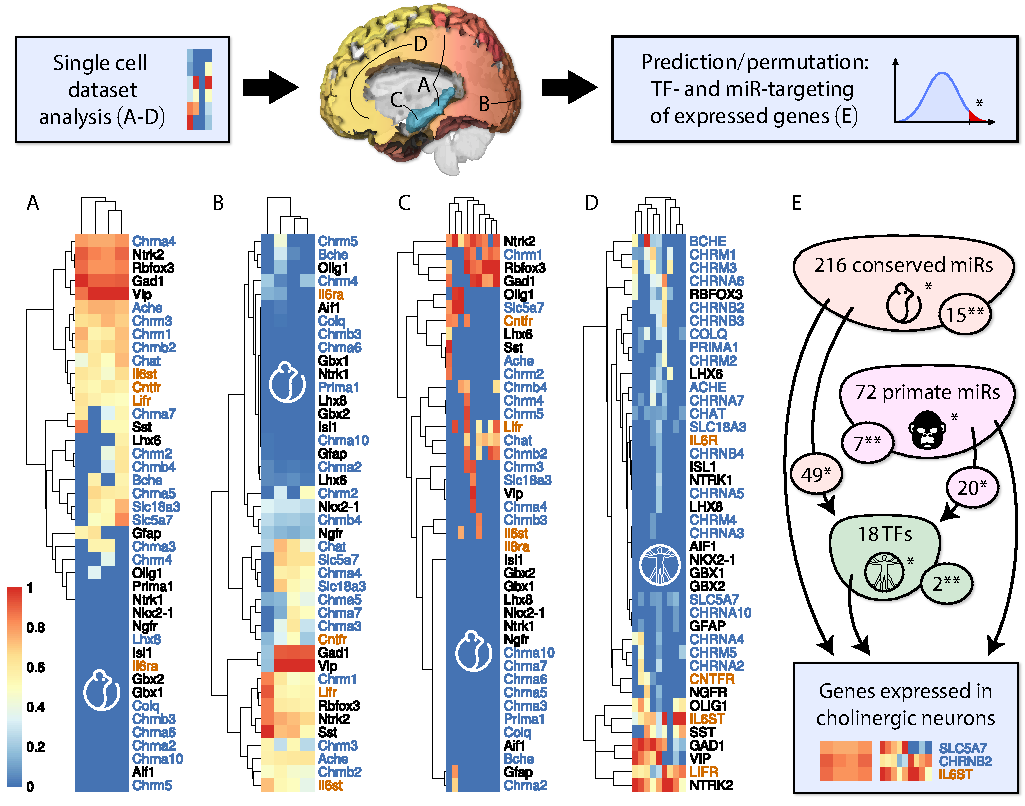
\includegraphics[width=\textwidth]{figures/singlecell}
\caption[Short figure name.]{This is a figure that floats inline and here is its caption.
\label{fig:singlecell}}
\end{figure}

Most cells identified as cholinergic by this definition expressed the general neuronal marker \textit{\acs{rbf}}, also known by its trivial name NeuN, but not the microglial marker \textit{\acs{aif}}. Few cells (or clusters of cells) expressed non-neuronal markers such as \textit{\acs{gfap}} (astrocytes) or \textit{\acs{oli}} (oligodendrocytes), hinting at sparse non-neuronal cholinergic functions. Cholinergic cells or clusters identified by the authors of the respective studies were classified as interneurons and co-expressed a number of known phenotypic neuronal markers, such as \textit{\ac{sst}} and \textit{\ac{vip}}.

Identified cholinergic cells also revealed a constant co-expression with neurokine-related genes, particularly the transmembrane neurokine receptors \ac{lifr} and \ac{ilst}, demonstrating a capacity to receive and process neurokine signals. In contrast, the high affinity receptor for \ac{ngf}, \textit{NTRK1}, is not expressed by many of the cholinergic neurons, fundamentally distinguishing these cells from the basal forebrain cholinergic projection neurons.
\todo{Clusters?}

\section{The Cellular Model}
A prominent example of human neuronal cell culture used in the identification and elucidation of cholinergic processes is the immortalised neuroblastoma cell line SH-SY5Y\cite{Biedler1978}. Derived from its parent line SK-N-SH, an adrenergic neuroblastoma\cite{Biedler1973}, it expressed ample amounts of \textit{\ac{ache}}, and thus had become a work horse in many cholinergic fields, such as Alzheimer's Disease (which is treated with \ac{ache} antagonists), pesticide development, and warfare(cite). However, in spite of its usefulness for processes involving \textit{\ac{ache}}, it turned out a less than optimal choice for the study of molecular events surrounding \textit{\ac{chat}} and \textit{\ac{slc}}, as it barely expresses both genes(cite), and cannot be coerced to elevate \textit{\ac{chat}} expression by the usual differentiation techniques (own experimentation, data not shown). Thus, for the questions asked in due course of this dissertation, SH-SY5Y does not qualify as adequate representation of a »cholinergic neuron«.

Following the elimination of SH-SY5Y as a suitable subject, I scoured the literature for candidates representing a cholinergic neuronal transcriptome, and found, among others, representatives of the LA-N neuroblastoma cell lines developed by R.C. Seeger around 1980\cite{Seeger1977, Seeger1982}. Neuroblastoma is a form of neuronal cancer often affecting small children, and, consequentially, the two cell lines used in my experiments are immortalised biopsies of a 3 year old girl (\acs{la2}\cite{Seeger1977}) and of a 4 month old boy (\mbox{\acs{la5}}\cite{Seeger1982}). The decision to use \ac{la2} as my initial cellular model was influenced by three factors: it is well described in literature, although most studies had been published in the 1980s and 90s; it expresses a substantial amount of \textit{\ac{chat}} and \textit{\ac{slc}}; and it responds to neurokine-mediated differentiation by assuming a neuronal morphology accompanied by further elevation of \textit{\ac{chat}} and \textit{\ac{slc}} expression. \ac{la5} was not nearly as well described as \ac{la2}, but later added to the experimental roster because of the complementary sex and hints towards cholinergic differentiation under retinoic acid\cite{Hill1997}.

\subsection{Culture}
LA-N cell culture is not as straightforward as many »go-to« human cell lines in today's laboratories. Because \ac{la2} and \ac{la5} are very similar in this regard, they were treated similarly and I will describe the procedure for both. They have comparatively high duplication times, which can be lowered by using certain conditions that affect medium composition, nutrition, and CO\textsubscript{2} content. The cells were acquired at DSMZ (Braunschweig, Germany), which recommends keeping them in a 50:50 mixture of \ac{dmem} and \ac{rpmi}, with 20\% \ac{fcs} added. Sometimes, recommendations also suggest Leibovitz's L-15 medium, which is specifically designed for low CO\textsubscript{2} conditions, and others have suggested increased CO\textsubscript{2} levels inside the incubator. I found a combination of the DSMZ-recommended medium with 8\% CO\textsubscript{2} atmosphere inside a 37°C incubator to accelerate growth to a degree that the cells could be split 1:3 to 1:4 in a weekly cycle. This protocol was used for all further experiments, which were performed between splits 2 to 8 after thawing of a batch from -80°C.

\subsection{Differentiation}
Neuronal differentiation of neuroblastoma cell lines has been performed in many instances, utilising a wide variety of differentiation agents such as the very general retinoic acid or 5-bromo-uracil, or very specific reagents, such as the neurokines \ac{il} and \ac{cntf}(cite). LA-N cells have also been described to react to a selection of these substances; however, due to the elevated interest in neurokine mechanisms, I chose to go ahead with a reagent from this group. Somewhat arbitrarily, I used \ac{cntf}, because upon my inquiry, James McManaman revealed in personal communication that the »\textit{\ac{chat}} development factor« that he had discovered\cite{McManaman1988} was, in fact, \ac{cntf}, which had never been published. Additionally, of the neurokines used for differentiation purposes, \ac{cntf} is best described in literature and easily acquired in dried form from Merck (Darmstadt, formerly SigmaAldrich, Germany).

LA-N cells are very sensitive to repeated temperature changes, which resulted in increased amounts of apoptotic cells following repeated removal from the incubator after seeding or medium changes during the experiment. For this reason, I chose to only add the differentiation reagent once, 24h after initial seeding of the cells into the wells of a 12-well-plate, and avoid further disturbances until time of lysis. For the maximum duration of my experiments, 120h from seeding until lysis, the initially supplied medium was sufficient for survival.

Differentiation was performed in regular growth medium without changes in \ac{fcs} content, and \ac{cntf} was added to the medium after an initial growth period of 24h. Cells were seeded into 12-well plates at approximately \num{200000} cells/well, with 1 ml of growth medium. To determine the optimal amount of \ac{cntf} for differentiation, time-dose-curves were determined for both cell lines in a range from \SIrange{1}{100}{\nano\gram\per\milli\litre}. Here, I discovered the first pharmacological difference between \ac{la2} and \ac{la5}: the maximum of their cholinergic response to neurokine stimulation (i.e., an elevation in \textit{\ac{chat}} and \textit{\ac{slc}} transcription) occurs at different concentrations of \ac{cntf}. While \ac{la2} cells respond most strongly to \SI{100}{\nano\gram\per\milli\litre}, \ac{la5} cells show an »inverted u«-type dose response with a maximum around \SI{10}{\nano\gram\per\milli\litre} \ac{cntf} (Fig. \ref{fig:dose-response}). James McManaman, who studied LA-N differentiation thoroughly in the 1990s\cite{McManaman1991}, believes both lines to respond in an »inverted u«-type manner (personal communication); thus, I assume that the \ac{la2} response would also diminish at \ac{cntf} concentrations significantly higher than  \SI{100}{\nano\gram\per\milli\litre}.
\subsection{RNA Isolation}
\section{Small RNA Sequencing and Differential Expression Analysis}
\subsection{microRNA Family Enrichment}
\section{Network Generation}
\section{The Cholinergic/Neurokine Interface}
\section{Application to Schizophrenia and Bipolar Disorder}

%!TEX root = ../dissertation.tex
\begin{savequote}[75mm]
I know words. I have the best words.
\qauthor{Donald Trump}
\end{savequote}

\chapter[Dynamics Between Small and Large RNA\texorpdfstring{\\}{} in the Blood of Stroke Victims]{Dynamics Between Small and Large RNA in the Blood of Stroke Victims}

Stroke is a dramatic incision into bodily homeostasis and affects a multitude of organ functions, first and foremost the brain. The immediate actions upon stroke are focused in preserving as much functional tissue as possible, so as to alleviate the cognitive damages resulting from neuron death. After this initial period of few hours, longer-lasting reactions determine the health and recovery of the patient. Many of these later events are related to immunity. The greatest danger to the patient after survival of the initial period are infections, such as pneumonia, usually between one and two weeks after the infarction. Pneumonia is often facilitated by aspiration of liquids or solids when the swallowing mechanism is impaired as a consequence of the cerebral damage. However, as introduced in Section \ref{sec:intro:stroke}, stroke-related immunodepression can play a role in post-stroke survival, and has been shown to have an impact on the transcriptome of blood-borne immune cells, at least for protein coding genes. The role of short RNA transcripts, and particularly of transfer RNA fragments, is much less clear.

\section{RNA Sequencing, Differential Expression, and Descriptive Methods}

We thus opted to analyse the blood of stroke victims taken upon hospitalisation and screen it for changes in small and large RNA expression.\todo{page break?}

\begin{method}

\subsection{The PREDICT Cohort}
The patient collective for the present study was recruited from a prospective, international, multi-center study with 11 study sites in Germany and Spain, led and approved by the neurologic department of Charité Berlin (www.clinicaltrials.gov, NCT01079728).\cite{Hoffmann2017} The study, called PREDICT, screened 484 stroke patients for clinical attributes and conventional biomarkers, with daily measurements in the first 5 days after stroke, and a three months follow-up. From these patients, a representative cohort of 49 patients were selected for blood small RNA sequencing. 

\subsection{Clinical Parameters Collected in the PREDICT Study}
Stroke patients were assessed daily for the duration of hospitalisation, at least until four days after admission. Blood-based biomarkers that were measured at least once during this period include: \ac{hladr}, interleukins IL-6, IL-8 and IL-10, IL-10 levels after 24h \emph{in vitro} stimulation with lipopolysaccharide, \ac{lbp}, \ac{mbl}, and \ac{tnf}-$\upalpha$. Also recorded were the time between admission and the collection of the blood sample, and the \ac{mrs}. This scale is a rough categorisation of the severity of stroke, with 0 referring to no symptoms, and 6 signifying death. Scores 1-2 describe slight neurological deficits, 3 requires frequent help because of medium level deficits, 4 requires constant assistance with daily tasks, and 5 requires stationary care.

\subsection{Sample Collection, RNA Isolation, and Sequencing}
Blood was collected into RNA stabilising tubes (Tempus Blood RNA tubes, Applied Biosystems) on each day of hospitalisation, and we subjected blood samples collected on the second day to small and large RNA-sequencing. While choosing samples for sequencing we only considered samples from patients with modified Rankin Scale (mRS) values of 3 and below at discharge from the hospital, to exclude very severe cases of stroke, leaving n=240 relevant cases. The time from stroke occurrence to blood withdrawal varied between 0.94 to 2.63 days, with an average of 1.98 days. Blood samples from age- and ethnicity-matched healthy controls were obtained at matched circadian time from donors with ethical approvals from institutional review boards (ZenBio, North Carolina, USA).

RNA was extracted from 3 ml of whole blood of all 484 PREDICT patients using the Tempus Spin RNA isolation kit (Invitrogen, Thermo Fisher Scientific, Waltham MA, USA). RNA quality was determined by RNA gel for all samples and by Bioanalyzer 6000 (Agilent, Santa Clara CA, USA) for samples selected for RNA-sequencing, which showed high RNA quality with a median RIN of 8.8 (lowest RIN 7.9, highest RIN 9.9). We used 600 ng total RNA of 49 samples for small RNA library construction (NEBNext Multiplex Small RNA library prep set for Illumina, New England Biolabs, Ipswich MA, USA) and selected 24 out of the 49 short RNA-sequenced samples for PolyA-selected mRNA sequencing. These libraries were prepared from 1000 ng total RNA using the TruSeq RNA library preparation kit (Illumina, San Diego CA, USA) and were sequenced on the Illumina NextSeq 500 platform at the Hebrew University’s Center for Genomic Technologies.

\subsection{RNA Sequencing Alignment} \label{sec:stroke:alignment}
Small RNA species were aligned after quality filtering using flexbar and miRExpress 2.0, as described in Section \ref{sec:cellculture:alignment}. Additionally, to assess tRF expression, small RNA reads were aligned to the exclusive tRNA space using the MINTmap pipeline.\cite{Loher2017} Briefly, this pipeline compares short RNA sequencing reads with a collection of sequences determined to only be contained inside mature tRNAs, without confounding from the many tRNA lookalikes in the human genome, e.g., in pseudogenes. The two RNA species were united into one expression matrix containing both miRNA and tRF expression.

Large RNA species were aligned to the human transcriptome (ENSEMBL transcriptome \emph{Homo sapiens} GRCh38 release 79) using the fast dual-phase parallel inference algorithm \emph{Salmon}.\cite{Patro2017} Briefly, the method combines an »online« fragment mapping utilising continuous updating of a Bayesian prior with an »offline« phase that determines fragment quantities by application of the Bayesian model determined before via a standard expectation maximisation (EM) algorithm or a variable Bayesian EM. Additionally, the pipeline corrects for multiple typical biases in sequencing, such as position-specific biases, sequence-specific 3' and 5' end biases, fragment GC content bias, and fragment length distribution. The resulting quantified fragments were imported into R using the rsubreads package.\cite{Liao2019}

\subsection{Quality Control and Filtering}
Raw and processed reads were quality-controlled using FastQC, as described in Section \ref{sec:cellculture:sequencing}, with no samples falling below acceptable thresholds. Small and large RNA alignments were batch-corrected followed by analysis of inter-sample relationships via the method proposed by Oldham \emph{et al.} (as described in Section \ref{sec:cellculture:quality}). We excluded no large RNA samples and one small RNA sample (»11\_40044\_S12«).

\subsection{RNA Sequencing Differential Expression Analysis}
Quantified reads were subjected to differential expression analysis using DESeq2, essentially as described in Section \ref{sec:cellculture:deseq}. Small RNA species were analysed together by combing count tables for miRNAs and tRFs, large RNA were analysed separately. Both datasets were corrected for covariates \emph{subject age} and \emph{batch}. Correction for patient sex was not necessary because all patients in the final analyses were male. Log$_2$-fold changes were shrunk using \emph{apeglm} as described in Section \ref{sec:cellculture:deseq}, at an alpha level of \emph{0.1}.

\subsection{Gene Ontology Analyses}
We performed \ac{go} analyses on the set of \ac{de} transcripts, using different ranking methods. GO analyses were performed using R/topGO as described in Section \ref{sec:cellculture:topgo} using the weighted method.

\subsubsection{Ranking by P-Value}
Transcripts were ranked by p-value, and different test sets were tested against the background of the topmost two thousand transcripts. We tested the set of all \ac{de} transcripts (adjusted p-value < 0.05) and the separate sets of positively and negatively regulated transcripts. Additionally, for each test group, the criterion of log$_2$-fold changes > 1.4 was applied and re-tested.

\subsubsection{Ranking By Count-Change}
Alternatively, transcripts were ranked by count-change, and the top 100 significantly \ac{de} transcripts were tested against the background of the first two thousand transcripts. Similarly to the p-value ranking, test sets comprised all transcripts as well as only negatively or positively regulated transcripts.

\subsection{Homology Computation Among tRNA Fragments}
Transfer RNA fragment origin can be ambiguous, even in fragments derived from tRNA-exclusive space. To assess sequence-based relationships between tRFs, all detected fragments were subjected to pairwise homology analysis using local Smith-Waterman alignment (\emph{pairwiseAlignment} function of the R/Biostrings package), and scores were transformed into a distance matrix to enable clustering and visualisation of relationships. t-SNE (t-Distributed Stochastic Neighbour Embedding) was employed to visualise tRF homologies in a 2D space.

\subsection{t-Distributed Stochastic Neighbour Embedding} \label{sec:stroke:tsne}
SNE (Stochastic Neighbour Embedding) replaces Euclidian distances between data points with conditional probabilities that represent similarities. The Gaussian distribution used in SNE to represent the probability density for any given data point in the low-dimensional space is replaced by a Student's t-Distribution in the updated t-SNE algorithm. In combination with the use of a symmetrised function with simpler gradients, this alleviates problems with optimisation of the cost function that is used to create forces between points on the low-dimensional map.\cite{Maaten2008}

t-SNE was used in a variety of applications to reduce the dimensionality of high-dimensional data, for instance, the amino acid origin of tRFs, or the association of tRFs with distinct cell types in the blood. t-SNE analyses were performed in R, using the Rtsne package.\cite{Krijthe2015} t-SNE requires, apart from the input data, a parameter called \emph{perplexity}, which determines the weighting of local as opposed to global effects in the data. So far, there are no strict rules governing the selection of a perplexity value, other than that the perplexity cannot exceed the number of individual data points. Since different perplexities can give widely varying results, which can sometimes be misleading, the resulting maps have to be screened with a range of perplexities to assess their robustness.

\subsection{Cholinergic Association of Small RNA Species} \label{sec:stroke:chol-assoc}
To determine association of distinct smRNAs with cholinergic transcripts, we analysed the multiple-targeting relationships of each distinct smRNA towards our curated list of \ac{ca} transcripts. We first created complete targeting data of all DE smRNAs towards all \ac{ca} transcripts, which we then successively filtered for multiple targeting behaviours. To assess the base level of multiple targeting of cholinergic transcripts, we utilised empirical cumulative density functions of the number of individual cholinergic targets of each miRNA and tRF (Figure \ref{fig:cholino-ecdfs}). We assumed 80\% to be a robust threshold of cholinergic targeting, and for diverging numbers between miRNAs and tRFs chose to use the higher (more stringent) threshold. smRNAs above this threshold (i.e., smRNAs targeting at least as many cholinergic transcripts as the threshold value) were considered \ac{ca}.

\end{method}

\begin{figure}
\includegraphics[width=\textwidth]{figures/cholino-ecdfs}
\caption[Cholinergic-associated Small RNA ECDF Curves.]{\textbf{Cholinergic-associated Small RNA ECDF Curves.} Cholinergic association was tested using \emph{miRNeo} targeting data of miRNAs and tRFs. To assess the best-suited threshold for defining cholinergic association, empirical cumulative density functions were calculated for the number of \acf{ca} genes targeted by each unique smRNA. \textbf{A)} Cumulative frequency of number of \ac{ca} genes targeted by tRFs. Threshold of 80\% (red line) is passed at five \ac{ca} genes targeted. \textbf{B)} Cumulative frequency of number of \ac{ca} genes targeted by miRNAs. Threshold of 80\% (red line) is passed at four \ac{ca} genes targeted.
\label{fig:cholino-ecdfs}}
\end{figure}

\section{Descriptive Analysis of RNA Dynamics in Blood After Stroke}

\subsection{Differential Expression of Large RNA}
At an alpha level of 0.05, we detected 694 \acf{de} long transcripts, 204 of them up- and 490 down-regulated (Figure \ref{fig:stroke-de-tsne}\,A). 18 of the up-regulated, and 109 of the down-regulated transcripts exceeded the common log$_2$-fold change threshold of 1.4. To determine the most-impacted pathways, we performed \ac{go} analyses.

\subsection{Gene Ontology Analyses of Differentially Expressed Genes} \label{sec:stroke:large-rna-go}
Ranking of all transcripts (regardless of direction of regulation) by their differential expression p-value resulted in GO terms mainly related to circulatory system processes (p = 0.018) and immunity. Most notable immune-related terms included cytokine-mediated pathways (p = \e{2.4}{-4}), response to \acp{ifn} $\upalpha$ (p = 0.013) and $\upbeta$ (p = \e{1.2}{-3}), regulation of JAK/STAT cascade (p = 0.013), response to \ac{lps} (p = 0.025), and macrophage activation (p = 0.026). Limiting the test set to transcripts with log$_2$-fold change above 1.4\,\,increased sensitivity towards immune processes, yielding lower p-values for the enrichment of of positive (\e{1.7}{-4}) and negative regulation of cytokine production (\e{5.7}{-4}), type I interferon production (\e{3.9}{-4}), response to bacterium (\e{5.9}{-4}), innate immune response (\e{2.0}{-3}), response to organophosphorous (\e{2.3}{-3}), cytoplasmatic pattern recognition receptor signalling pathway (\e{2.8}{-3}), and response to \ac{lps} (\e{9.1}{-3}).

Up-regulated transcripts pertained to circulatory system processes, such as platelet degranulation (\e{1.2}{-3}) and aggregation (0.02), and sprouting angiogenesis (\e{4.8}{-3}), but also antigen processing and presentation (\e{4.5}{-3}). Test set limitation to log$_2$-fold change above 1.4 did not increase sensitivity of those terms, but presented essentially similar results. Up-regulated genes as such might be indicative of the bodily response to blood flow disruption and ischaemia caused by the stroke. 

Down-regulated transcripts were enriched in terms involving response to \ac{ifn} $\upalpha$ (\e{1.3}{-3}) and $\upbeta$ (\e{3.1}{-4}), response to \ac{lps} (\e{1.5}{-3}), rhythmic process (\e{2.5}{-3}), positive regulation of T cell proliferation (\e{4.3}{-3}), positive regulation of JAK-STAT cascade (0.015), and cellular response to \ac{il}-1 (0.019). Test set limitation to log$_2$-fold change above 1.4 again increased sensitivity towards immune-related terms, but without changing the general pattern. Thus, down-regulated genes in all likelihood represent the post-stroke immunodepression, which can exacerbate into CIDS (see Section \ref{sec:intro:stroke}). The terms involving INF, IL-1, LPS, and JAK-STAT also indicate an important role for cytokine signalling in these processes.

As a cross-check, \ac{de} transcripts were ranked by count-change, and re-analysed. The top 100 changed transcripts, without regard to direction (absolute count-change) yielded terms implying response to \ac{ifn} $\upalpha$ (\e{3.8}{-4}), $\upbeta$ (\e{1.1}{-4}), and $\upgamma$ (\e{1.4}{-4}), mitochondrial organisation (\e{5.6}{-3}) and ATP synthesis (\e{6.9}{-3}), response to \ac{il}-4 (\e{6.9}{-3}), positive regulation of JAK-STAT cascade (\e{8.8}{-3}), response to antibiotic (0.044), and platelet degranulation (0.045). The top 100 up-regu"-la"-ted transcripts yielded terms involving platelet degranulation (\e{3.8}{-3}), mitochondrial ATP synthesis (\e{4.2}{-3}), response to xenobiotic stimulus (0.017), platelet aggregation (0.013), and response to antibiotic (0.016), while the top 100 down-regulated transcripts were associated with inflammatory response (\e{1.3}{-4}), regulation of apoptosis (\e{1.8}{-4}), cytokine secretion (\e{6.8}{-4}), antigen processing and presentation (\e{1.2}{-3}), regulation of lymphocyte apoptosis (\e{2.3}{-3}) and proliferation (\e{2.7}{-3}), response to antibiotic (\e{5.2}{-3}), leukocyte homeostasis (\e{7.6}{-3}), response to \ac{il}-1 (\e{7.6}{-3}), and many more immune-specific processes. This corroborates the previous findings, that up-regulated transcripts represent the response to circulatory system damage, and down-regulated transcripts indicate a cytokine-mediated immunodepression. For a full list of all terms from these analyses\todo{DE genes?}, see Appendix \ref{appendix:go-terms-large-rna}. 

\subsection{Differential Expression of small RNA}
In the simultaneous co-analysis of miRNAs and tRFs, we detected 420 DE miRNAs and 143 DE tRFs (adjusted p-value < 0.05, Figure \ref{fig:stroke-de-tsne}\,B\&C). 63\% of miRNAs (265) were down-regulated, while 87\% of tRFs (124) were up-regulated. tRFs were mainly derived from the 3' end (3'-tRFs, 87) or from internal tRNA regions (i-tRFs, 48), while the tRFs from 5' ends (5'-tRFs) were in the minority (6). The amino acid distribution was shifted in favour of alanine- (35), glycine- (28), and proline-carrying (12) tRNAs (Figure \ref{fig:stroke-de-tsne}\,D). 30 of the 35 alanine-associated tRFs were 3'-tRFs, and all of those were up-regulated, indicating non-random generation of these fragments.

\begin{figure}[ht]
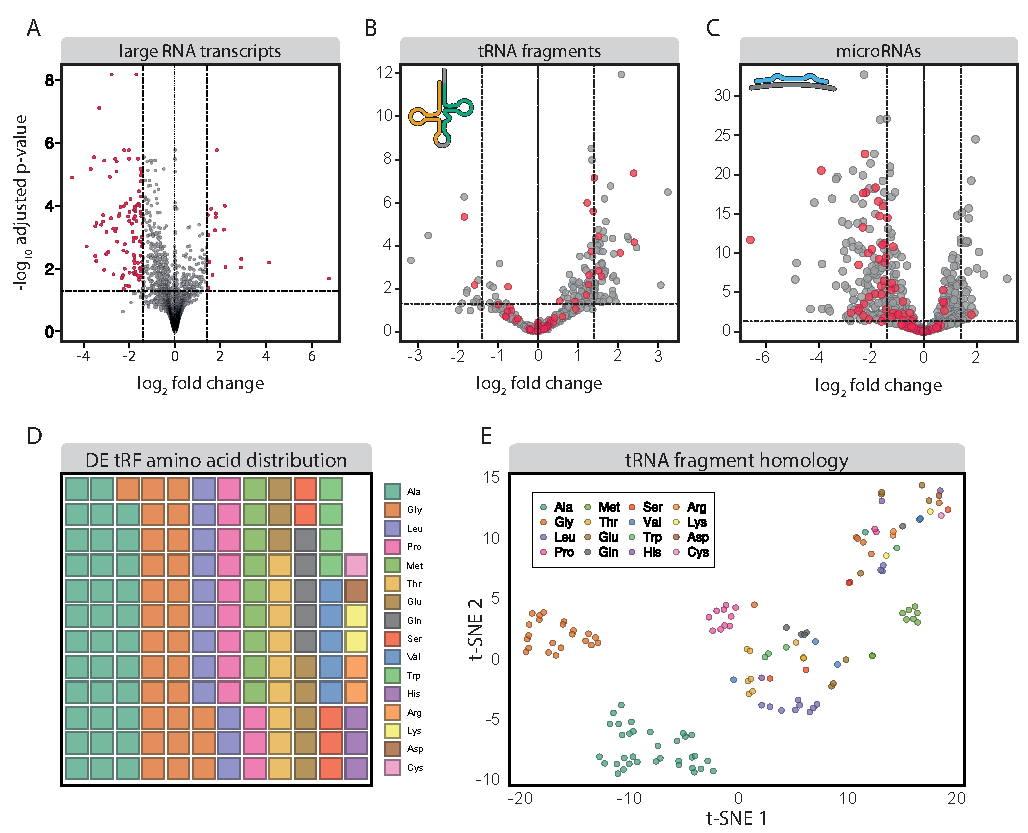
\includegraphics[width=\textwidth]{figures/stroke-de-tsne}
\caption[Small and Large RNA Differential Expression and tRF Properties.]{\textbf{Small and Large RNA Differential Expression and tRF Properties.} \textbf{A)} Differential expression analysis reveals multiple large RNA transcripts changed in patient blood after stroke. The majority of differentially expressed (DE) transcripts above a log$_2$ fold change threshold of 1.4 (red) are down-regulated. \textbf{B)} Blood-borne tRNA fragments (tRFs) also change after stroke. Unlike large RNA and miRNAs, the majority of DE tRFs are up-regulated. \Acf{ca} tRFs in red. \textbf{C)} Blood-borne miRNAs are heavily influenced by the events following stroke. Like large RNA transcripts, miRNAs are also overwhelmingly down-regulated. \Ac{ca} miRNAs in red. \textbf{D)} The distribution of amino acid origin among the DE tRFs is non-random and biased towards the amino acids alanine, glycine, leucine, proline, and methionine. Each square represents one DE tRF, colour denotes amino acid origin. \textbf{E)} t-SNE of pairwise fragment homology by local Smith-Waterman alignment shows clustering of the dominant amino acid groups of tRFs. Clear clusters can be observed for tRFs derived from tRNA carrying alanine, glycine, leucine, proline, and methionine.
\label{fig:stroke-de-tsne}}
\end{figure}

\subsection{Homology Among tRNA Fragments}
Using pairwise homology among all DE tRFs, visualised via t-SNE (see Section \ref{sec:stroke:tsne}), we identified clusters of highly similar fragments, that correlate with their amino-acid origin, i.e., the amino acid which is carried by the respective parent tRNA (Figure \ref{fig:stroke-de-tsne}\,E). This relationship persisted across distinct individual tRNAs coding for the same amino acid, and was particularly pronounced in tRNAs associated with alanine, glycine, leucine, proline, and methionine.

\subsection{Cholinergic Association of Small RNA Species}
The association of smRNA species to distinct systems or pathways is not trivial because of the multiple-targeting nature of these RNAs. For the purpose of the following analyses, we define a small RNA as being associated with cholinergic processes by the positive association of the smRNA with a number of \acf{ca} large transcripts. We do not assess the question whether this small RNA also targets other systems equally, or even if it targets cholinergic transcripts with greater likelihood than a random selection of genes. For this reason, we select a fairly high threshold for the definition of a \ac{ca} smRNA, which is the targeting of at least 5 \ac{ca} transcripts (above 80\% on the empirical cumulative density function of cholinergic targeting, see Section \ref{sec:stroke:chol-assoc}).

Following this definition, we detected 52 \ac{ca} miRNAs (90\% down-regulated, 5 up and 47 down), and 18 \ac{ca} tRFs (83\% up-regulated, 15 up and 3 down). Above a threshold of log$_2$-fold change of 1.4, we found 33 \ac{ca} miRNAs (97\% down-regulated, 1 up and 32 down), and 9 \ac{ca} tRFs (78\% up-regulated, 7 up and 2 down). \ac{ca} smRNAs are marked in red in Figure \ref{fig:stroke-de-tsne}\,B\&C.\todo{amino acids?}

\section{Blood Compartments of Cholinergic Systems and Small RNA Species}
To address the shortcomings of whole-blood RNA sequencing, which is more representative of the clinical setting, but less specific regarding cellular compartments, we consulted third party datasets to assess RNA species distribution in different cellular and non-cellular compartments of the blood. For small RNA species, we re-analysed a published dataset of small \ac{seq} of 450 human samples from various blood tissues;\cite{Juzenas2017} for large RNA transcripts, we utilised the tissue specificity of Marbach's regulatory circuits.\cite{Marbach2016} The large RNA information was used to identify blood cell types with cholinergic transcriptional activity, which was then used to zoom in to small RNA expression subsets related to cholinergic processes.

\begin{method}

\subsection{Large RNA Regulatory Circuits in Tissues of the Blood}
To evaluate the cell type distribution of cholinergic genes in blood tissue types, we utilised the expression patterns derived from cumulative transcription factor activity of Marbach's regulatory circuits.\cite{Marbach2016} As shown by the authors, the cumulative activity of all transcription factors towards one gene describe well the actual expression of that gene in the respective tissue type. To maximise comparability to the parallel analyses of small RNA species (Section \ref{sec:stroke:juzenas}), blood cell types (i.e., »regulatory circuits«) were selected to reflect the cell type selection of Juzenas \emph{et al.}\cite{Juzenas2017} based on similar markers of the »cluster of differentiation« family of genes. These were: CD4-positive T-helper cells, CD8-positive cytotoxic T-cells, CD14-positive monocytes, CD15-positive neutrophils, CD19-positive B-cells, CD56-positive natural killer cells, and, for comparison, whole blood. For the sake of simplicity, genes were considered »present« in each blood tissue type if at least one TF showed activity towards the gene.

TF activities were collected for all of the tissues and aggregated across all genes by summing. The resulting table of 15\,032 genes in the seven tissues was used as input for the \emph{Rtsne} function.\cite{Krijthe2015} t-SNE was computed using a perplexity of 49 and visualised as 2D map using R/ggplot2.\cite{Wickham2016}

\subsection{An Atlas of Small RNA Expression in Cell Types of the Blood} \label{sec:stroke:juzenas}
To evaluate the cell type distribution of our small RNA molecules, we analysed a dataset deposited by Juzenas \emph{et al.},\cite{Juzenas2017} who separated and sequenced 450 samples comprising seven types of individual blood cell types (characterised by »cluster of differentiation«-type membrane-bound receptors), serum, exosomes, and whole blood. The individual blood cell types comprised CD4-positive T-helper cells, CD8-positive cytotoxic T-cells, CD14-positive monocytes, CD15-positive neutrophils, CD19-positive B-cells, CD56-positive natural killer cells, and CD235a-positive erythrocytes (the only distinct cell type not available in Marbach's regulatory circuits, since mature erythrocytes do not transcribe). Starting from the raw data deposited on NCBI GEO, we controlled the quality, applied quality based filtering, and aligned the 450 samples to miRNA and tRF sequences, as described in Section \ref{sec:stroke:alignment}. The original publication did not offer statistical analyses because of a failure in the spike-in procedure, and defined presence of a small RNA by a measure of at least five counts in 85\% of samples. However, since this definition relies heavily on sequencing depth, and depth can vary widely even in methodically robust sequencing experiments depending on a large number of variables (see Figure \ref{fig:read-quality-length}\,C), we defined our own test for descriptive analysis of presence or absence of lowly expressed small RNAs in each of the sample types:

\subsection[Definition of Presence and Absence of Lowly Expressed\texorpdfstring{\\}{} smRNA Molecules]{Definition of Presence and Absence of Lowly Expressed smRNA Molecules}
This definition comprises estimation of a log-normal distribution from a small RNA expression profile, and a statistical test to refute the null hypothesis that the distribution is in fact log-normal. The danger of evaluating true expression of lowly expressed smRNA molecules by a count-based threshold is the possibility of random reads resulting from degradation products of highly expressed RNA with similar sequence, and the amplification of noise. Both problems are exacerbated by an increase in sequencing depth. In today's \ac{seq} technology, most chips can accommodate only a limited amount of samples compared to the amount of reads that can be generated. While this is not as problematic in cases of longer inserts and paired design, which is usually employed in large \ac{seq}, in small \ac{seq} this can lead to enormous overheads of reads. It is not uncommon to receive tens of millions of reads for each sample, which exceeds the recommended amount (of at least one million) by large margins.

Thus, there is the need to distinguish between degradation products of highly expressed RNA molecules or amplified noise and legitimate lowly expressed smRNA molecules (even more so since one of the smRNA species is a product of non-random tRNA degradation). The central assumption for our proposed method is: The expression pattern of legitimate smRNA molecules follows, as is common in biology, a normal distribution of some kind, or, for the discrete case, a normal poisson distribution. On the other hand, degradation products or noise would rather follow other, »non-biological« distributions, such as a uniform distribution or a monotonously decreasing power-law distribution such as the Pareto distribution. Thus, we chose to statistically test each smRNA in each tissue type for the adherence to this criterion, by comparing the measured counts with a distribution function estimated based on the mean and standard deviation of the measured counts. During testing, we found the log-normal distribution to give the best classification results.
 
The distribution mean and standard deviation of the expression values per cell type and smRNA were estimated using the \emph{fitdist} function of the R/fitdistrplus package.\cite{Delignette-Muller2015} The count distribution was then tested against a log-normal distribution with the estimated mean and standard deviation via the R implementation of the Kolmogorov\=/Smirnov test, with a cutoff of 0.1. The small RNA was defined as present if the test failed to reject the null hypothesis (see Appendix \ref{appendix:presence-absence} for numerous examples).

\subsubsection{Analysis of Expression Patterns and Establishment of Virtual Tissues}
The distribution of smRNA expression across the different cell types was used to assign 8 functional compartments (i.e., »virtual tissues«) to the entirety of detected fragments such that each smRNA was sorted into one of the tissue classes. Ideally, these classes would be unambiguous, i.e., there would be no overlap of smRNA molecules between the classes. Eight classes were created via hierarchical clustering of miRNA and tRF expression separately (Figure \ref{fig:heatmaps-small}), and then used in combination with t-SNE applied to the entire expression matrix, to visualise the compartmentalisation of smRNAs in these virtual tissues. The samples taken from stroke patients in the PREDICT study were sequenced from whole blood, which precludes direct information about tissue distribution. Thus, the two-dimensional maps from t-SNE visualisation were used to, first, explore the tissue association of smRNAs differentially expressed in stroke patients' whole blood samples, and second, examine the potential impact of \acl{ca} smRNAs in these tissues.

\end{method}

\subsection{Large RNA Expression Patterns Identify Cholinergic Systems\\ in CD14-positive Monocytes}
The expression patterns of 15\,032 large RNA molecules in blood-borne immune cells were visualised in a t-SNE-derived 2D map (Figure \ref{fig:tsne-large}\,A). More than half of all transcripts show highest expression in whole blood (7533, not shown), so subsequent analyses were performed on the set of six tissues, without the whole blood compartment. In this set (14\,280 genes), most transcripts show highest expression in monocytes (9125 transcripts), followed by CD19-positive B-cells (1176) and neutrophils (1166). Remaining are CD4-positive T-helper cells (1092), NK-cells (948), and CD8-positive cytotoxic T-cells (773). When filtered for cholinergic genes, there is visible enrichment of core cholinergic transcripts in a spatial sub-compartment of CD14-positive monocytes (Figure \ref{fig:tsne-large}\,B). Considering the different monocyte phenotypes (pro- and anti-inflam"-ma"-to"-ry, see Section \ref{sec:intro:stroke}), and their implied transcriptomic differences, which most likely are brought on by divergent TF activity, this compartmentalisation of cholinergic transcripts inside one spatial sub-compartment might indicate a cholinergic »preference« in favour of one particular monocyte phenotype. 

\begin{figure}
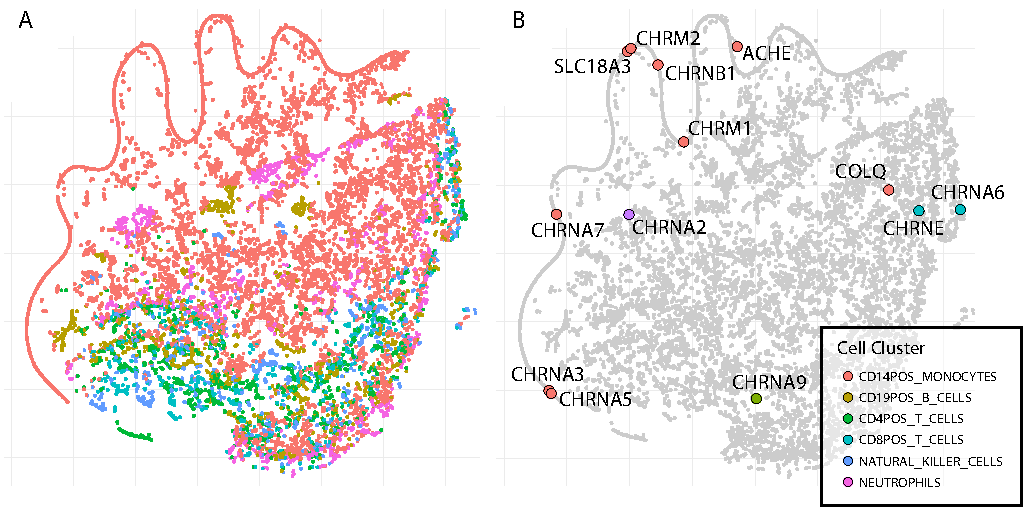
\includegraphics[width=\textwidth]{figures/tsne-large}
\caption[Large RNA Expression Patterns in Blood-Borne Cells.]{\textbf{Large RNA Expression Patterns in Blood-Borne Cells.} Expression derived from transcriptional activity in blood-borne cell types in the Marbach dataset\cite{Marbach2016} was visualised via t-SNE. The input matrix comprised all 14\,280 detected genes in 6 types of blood-borne immune cells. Genes were plotted on the first two t-SNE dimensions and coloured by the cell type of their highest expression, i.e., the highest cumulative transcriptional activity of all active TFs. \textbf{A)} Complete t-SNE shows a gradient of expression across the different cell types, with much expression in CD14-positive monocytes and T-cells. \textbf{B)} Highlighting of cholinergic core genes reveals an enrichment in close compartments of CD14-positive monocytes. The vesicular ACh-transporter SLC18A3 can serve as substitute for the main cholinergic marker, CHAT, as discussed in Section \ref{sec:database:tf}.
\label{fig:tsne-large}}
\end{figure}

\subsection{Identification of Functional Enrichment of smRNA Expression\\ in Blood-Borne Cells}
To date, there is no comprehensive expression catalogue of smRNA species expression in the tissue types of the human body that is comparable to what has been achieved in the description of large RNA. To classify the detected smRNAs in a manner specific to tissues in human blood, we utilised a dataset published by Juzenas \emph{et al.},\cite{Juzenas2017} who describe miRNA expression in a variety of blood tissues (see Section \ref{sec:stroke:juzenas} for details). We re-analysed the publicly deposited data for miRNA and tRF expression, and developed our own method of defining »presence« of the smRNA in each tissue type based on the evaluation of a log-normal distribution model (instead of using a simple count threshold). 

Using this presence/absence data, we first utilised hierarchical clustering to establish »virtual tissues« that could be assigned to each smRNA (Figure \ref{fig:heatmaps-small}) for later evaluation in the stroke patient sequencing. Both miRNAs and tRFs showed a number of clearly associated smRNAs with several compartments, whereas other compartments and smRNAs were distributed in a more complex manner. The ten tissue types of the Juzenas \emph{et al.}\cite{Juzenas2017} study were equally parted into two five-tissue superclusters by the expression patterns of both smRNA species (Figures \ref{fig:heatmaps-small}\,A\&B, x-axis). These two clusters distinguish immune from non-immune compartments in the blood, but for one notable exception: while the »immune supercluster« comprises monocytes, T-cells, B-cells, and NK-cells, the »non-immune supercluster« contains neutrophils in addition to erythrocytes and the non-cellular tissues serum, exosomes, and whole blood. Notably, the neutrophil samples cluster closest to the whole blood compartment in both smRNA species.

Two distinct virtual tissues showed high consistency in both smRNA species: a virtual tissue containing only CD14-positive monocytes and another tissue comprising all studied cellular immune components except neutrophils (i.e., monocytes, B-cells, CD4- and CD8-positive T-cells, and NK-cells). miRNAs (Figure \ref{fig:heatmaps-small}\,A), in addition, yield clear clusters for whole blood expressed miRNAs, and for miRNAs expressed ubiquitously without exception. In tRFs (Figure \ref{fig:heatmaps-small}\,B), the general picture is more complicated, as the clusters are often mixed.

\begin{figure}
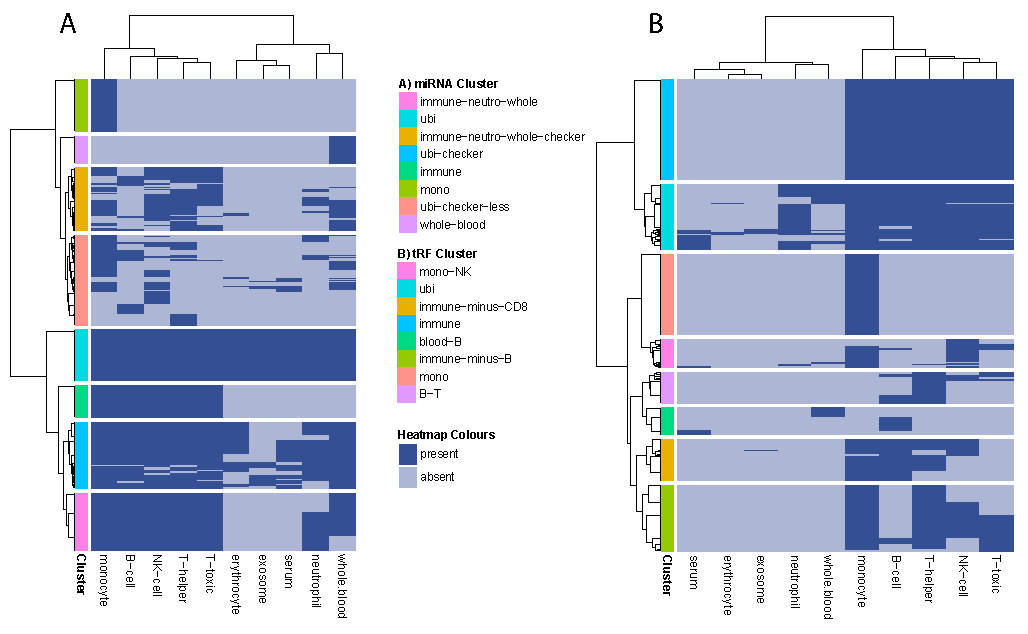
\includegraphics[width=\textwidth]{figures/heatmaps-small}
\caption[Functional Characterisation of Hierarchical Clusters in Blood Cell Small RNA Expression.]{\textbf{Functional Characterisation of Hierarchical Clusters in Blood Cell Small RNA Expression.} Information on presence/absence of miRNAs and tRFs in the tissue types analysed in Juzenas \emph{et al.}\cite{Juzenas2017} were hierarchically clustered into 8 clusters using the Ward method,\cite{Ward1963} and plotted on a heatmap (single smRNAs on the y-axis, tissue types on the x-axis). To assign meaning to these clusters, manual inspection was followed by annotation of enrichment in tissue types. Complex combinations were approximated by their most prominent features. \textbf{A)} Clusters of miRNA presence/absence in blood cell compartments. Clearest cluster association was shown by miRNAs expressed only in monocytes (»mono«), in all blood-borne immune cells except neutrophils (»immune«), ubiquitously without exception (»ubi«), and only in whole blood (i.e., in none of the single compartments (»whole-blood«). \textbf{B)} Clusters of tRF presence/absence in blood cell compartments. Clearest cluster association was shown by tRFs expressed only in monocytes (»mono«), and in all blood-borne immune cells except neutrophils (»immune«). The other tissue-related clusters were not as clear as in the miRNA expression data, indicating a looser association to cell type of tRNA-derived smRNAs.
\label{fig:heatmaps-small}}
\end{figure}

\subsection{Expression Patterns of Differentially Expressed and\\ Cholinergic-Associated smRNAs}
Similarly to the visualisation of large RNA molecules, the expression patterns of 600 miRNAs and 1671 tRFs in ten tissues of the blood were visualised in t-SNE-derived 2D maps (Figure \ref{fig:tsne-small}\,A\&B). In the initial visualisation, the forming of multiple clusters according to some virtual tissues can be observed, while other virtual tissues are visibly more dispersed. Clearest clusters are formed in both cases by ubiquitously expressed smRNAs (»ubi«), smRNAs expressed only in monocytes(»mono«), and smRNAs equally expressed in all immune-related blood-borne cells except for neutrophils (»immune«). Examination of DE smRNAs on this 2D map shows a further parallel between miRNAs and tRFs (Figure \ref{fig:tsne-small}\,C\&D): differential expression after stroke takes place in all compartments of the blood, and highest changes in transcript amount (as measured by count-change) are observed in ubiquitously expressed smRNAs. Similarly, \ac{ca} miRNAs and tRFs (Figure \ref{fig:tsne-small}\,E\&F) are observed in all compartments, but the most highly differentially regulated CA smRNAs are expressed in all blood tissues alike. Notably, whole blood does not play a role in DE miRNAs, which might indicate lower relative importance of non-cellular blood compartments in terms of classification. In other words, most smRNAs that are found in non-cellular compartments are found in the cellular compartments as well, making them irrelevant for classification (however, their biological function in these non-cellular compartments remains a matter of interest).

\begin{figure}
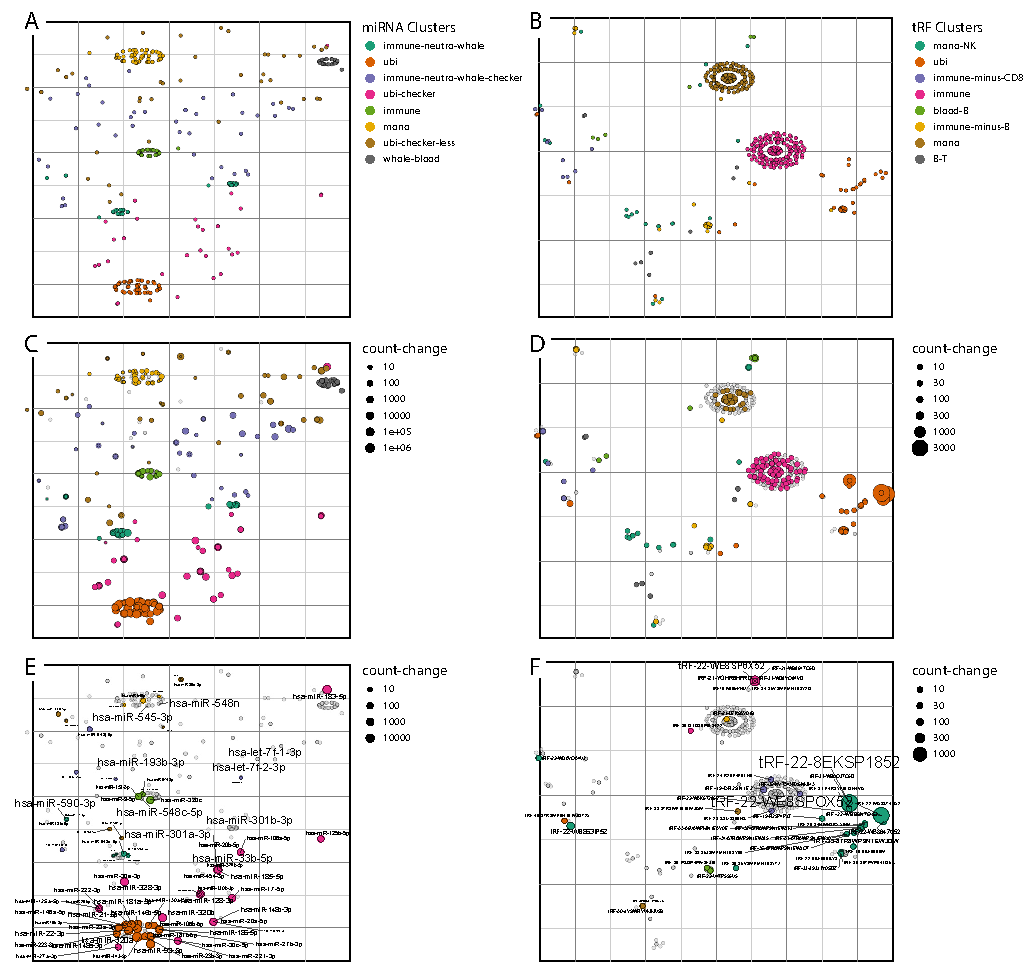
\includegraphics[width=\textwidth]{figures/tsne-small}
\caption[Small RNA Expression Patterns in Blood-Borne Cells.]{\textbf{Small RNA Expression Patterns in Blood-Borne Cells.} Two-dimensional expression maps were created using t-SNE on the full numeric expression data derived from re-analysis of the Juzenas \emph{et al.}\cite{Juzenas2017} data set for miRNAs and tRFs separately. Single smRNAs (points) were coloured by the virtual tissues derived from the cluster heatmap analysis (Figure \ref{fig:heatmaps-small}). Node size reflects absolute count change in C), D), E), and F). Shown are full data, differentially expressed (DE) smRNAs, and \acf{ca} smRNAs for each species. \textbf{A)} Full t-SNE visualisation of miRNA expression. The largest 2D-associative clusters are comprised of the clearest presence/absence virtual tissues, monocytes (yellow) and ubiquitously expressed (orange). Smaller clusters can be identified for the tissue of all immune cells except neutrophils (green) and the complex cluster of immune cells including neutrophils and whole blood (turquoise). \textbf{B)} Full t-SNE visualisation of tRF. The largest 2D-associative clusters are, as in miRNAs, comprised of the clearest presence/absence virtual tissues, monocytes (brown) and immune cells except neutrophils (pink). A smaller cluster can be identified for ubiquitously expressed tRFs (orange). \textbf{C)} miRNAs \ac{de} after stroke are ubiquitously expressed in all virtual tissues. Highest differential expression is seen in the »ubi« cluster. \textbf{D)} Likewise, tRFs \ac{de} after stroke are ubiquitously expressed in all virtual tissues, and highest differential expression is seen in the »ubi« cluster. \textbf{E)} \Ac{ca} miRNAs are enriched in the lower quadrants of the 2D map, particularly in the clusters associated with ubiquitous expression (»ubi«, »ubi-checker«). \textbf{F)} \Ac{ca} tRFs show a similar distribution, skewed towards virtual tissues with ubiquitous expression. This indicates covariation of detection with broadness of expression (see text).
\label{fig:tsne-small}}
\end{figure}

\section{Regulatory Circuits of Small RNA and Transcription Factors\\ in CD14-positive Monocytes}

\begin{method}

\subsection{Comprehensive Circuit Network Creation} \label{sec:stroke:circuit-network}
The comprehensive transcriptomic network in CD14-positive monocytes was created in a two-step process of \emph{miRNeo} targeting. First, the complete TF$\to$gene network was created from the targeting data derived from Marbach \emph{et al.}\cite{Marbach2016}, yielding a CD14-specific network comprising 616 TFs with activity towards 13\,447 transcripts, in 318\,731 unique interactions. Second, this network was then subjected to successive \emph{miRNeo} targeting of all transcripts in the network by miRNAs and tRFs.

For each node fulfilling an active role in this network (i.e., miRNAs, tRFs, and TFs), an activity parameter was computed. The activity of each node is hereby defined as the sum of all scores of each of its targeting relationships. In the case of miRNAs, the score is the summary score introduced in Section \ref{sec:database:mirna}, for tRFs, it is the score calculated with the BL-PCT method (see Section \ref{sec:database:trf-targeting}), and for TFs, it is the transcriptional activity given by Marbach \emph{et al.}\cite{Marbach2016} Activities were normalised, for each biotype separately, by scaling the calculated values $v$ onto a range between 0 and 1, using $$v_{i, norm} = \frac{v_i}{max(v)}$$
with $max(v)$ being the maximum of all scores in this biotype category, and all $v$ > 0. The activity of each relationship determined the weight of the edge between the two connected nodes.

The network was visualised in gephi,\cite{Jacomy2014} omitting all non-TF genes, and using ForceAtlas2 to generate a force-directed 2D map of smRNA$\to$TF interactions in CD14-positive monocytes. Network modularity was calculated using the function included in gephi, with a resolution of 2.0, to yield 2 distinct modularity classes. The module association of TFs to the tRF- and miRNA-associated modules were used to perform subsequent analyses of the distinct modules. 

\subsection[Gene Ontology Analyses of TF$\to$Gene Networks\texorpdfstring{\\}{} of CD14-positive Monocytes]{Gene Ontology Analyses of TF$\to$Gene Networks of CD14-positive Monocytes} \label{sec:stroke:go-cd14}
The TF$\to$gene networks of each of the two modules derived from smRNA species association (miRNAs versus tRFs) were analysed using topGO\cite{Alexa2006} essentially as described in Section \ref{sec:cellculture:topgo}. Genes were ordered according to the cumulative activity of TF targeting of each gene in CD14-positive monocytes. To display a range of top genes, transcript background was iterated in five equal steps from 1000 transcripts to the maximum size of target transcripts in each network (12\,927 for miRNA-targeted TFs, 12\,904 for tRF-targeted TFs). The test set was the top 10\% of transcripts for each background size. GO terms were collected and screened for multiple entries among the sets. The most prevalent terms were used to infer the functional roles of miRNA- and tRF-targeted transcription factors. We determined the overlap of GO terms between both smRNA species as well as the terms exclusive to either. 

\end{method}

\subsection{Dichotomy of Small RNA Targeting of Transcription Factors\\ in CD14-positive Monocytes}
Organisation of the smRNA$\to$TF network via a force-directed algorithm resulted in visible clustering of two distinct subnetworks, that are governed by miRNAs and tRFs, respectively (Figure \ref{fig:smrna-tf-network-fractions}). Inside this network, 10 TFs were found DE in patient blood after stroke (Figure \ref{fig:smrna-tf-network-fractions}\,A). Calculation of modularity clearly divided the network into TFs primarily influenced by miRNAs and TFs primarily influenced by tRFs (Figure \ref{fig:smrna-tf-network-fractions}\,B). Based on these two sets of TFs, two distinct TF$\to$gene networks were created: 289 miRNA-biased TFs with 152\,649 unique TF$\to$gene targeting relationships, and 280 tRF-biased TFs with 163\,641 unique TF$\to$gene targeting relationships.

\subsection{Gradual Shift in Control Over Transcription Factors\\ by miRNAs and tRFs}
Of those TFs, 356 were detected in the stroke patient blood sequencing experiment. It is notable that, although the complete graph shows clear segregation between miRNA-targeted and tRF-targeted transcripts, merely 106 of those TFs are targeted by only one of the two smRNA species (48 only by miRNAs and 58 only by tRFs), and 55 are supposedly not at all targeted by any smRNA present in CD14-positive cells. The remaining 195 TFs are putative targets of both smRNA species (Figure \ref{fig:smrna-tf-network-fractions}\,C). 

At an alpha level of 0.1 for the differential expression between stroke patients and controls, 26 of these TFs remain, also showing a gradual pattern of targeting by miRNAs and tRFs (Figure \ref{fig:smrna-tf-network-fractions}\,D). Six of these transcription factors are implicated in the control of cholinergic core or receptor genes (marked with a »C«). It is notable that a number of TFs show no indication of being a target of either smRNA species present in CD14-positive cells under the premises of this dissertation's targeting approach (Figure \ref{fig:smrna-tf-network-fractions}\,E). Considering the multiple-targeting behaviour of smRNAs, and the general experience that non-targeted genes are uncommon, this finding is interesting in itself, particularly since it involves well described regulators of immunological processes, such as \emph{STAT2} and \emph{ELF1}.

\begin{figure}
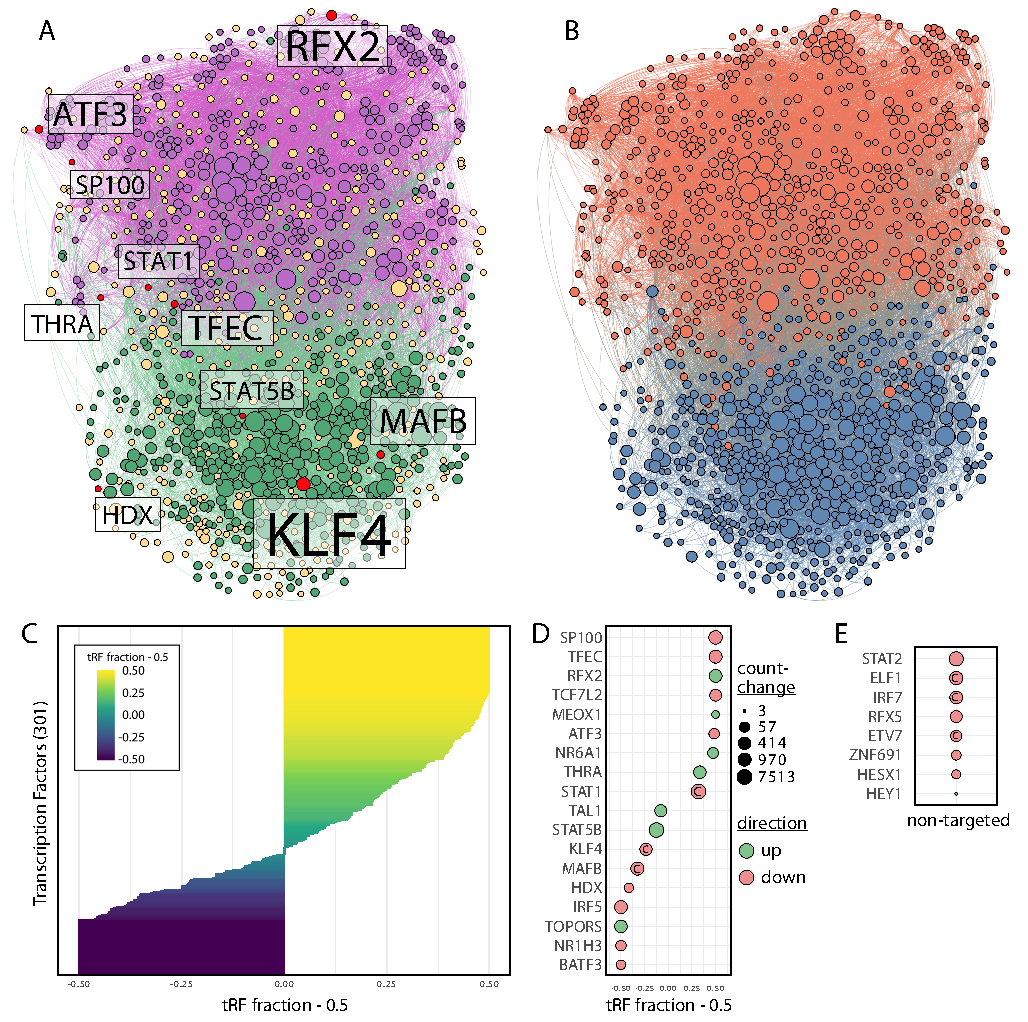
\includegraphics[width=\textwidth]{figures/smrna-tf-network-fractions}
\caption[Small RNA Targeting of Transcription Factors in CD14-positive Monocytes.]{\textbf{Small RNA Targeting of Transcription Factors in CD14-positive Monocytes.} The two-dimensional map of all TFs active in CD14-positive monocytes and their smRNA controllers was created via \emph{miRNeo} targeting and visualisation via force-directed algorithm. Node size is determined by activity (see Section \ref{sec:stroke:circuit-network}). \textbf{A)} Nodes coloured by biotype: miRNAs - green, tRFs - purple, TFs - yellow, differentially expressed TFs: red. TFs targeted mainly by tRFs segregate visually from TFs targeted mainly by miRNAs. Both sets contain DE TFs, indicating complementary function. \textbf{B)} The network was segregated into two modules by network connectivity measures. Node colour denotes modularity class association. Network modularity largely reflects TF targeting of tRFs (orange) versus miRNAs (blue). \textbf{C)} Bar graph displays the fraction of smRNAs of each species targeting each of the TFs. A tRF fraction of 1 means all smRNAs targeting the TF are tRFs, 0 means all are miRNAs. Displayed on x axis is »tRF fraction - 0.5« to center on 50:50 targeting by both species. 48 TFs are solely targeted by miRNAs (leftmost) and 58 solely by tRFs (rightmost). \textbf{D)} Similarly, TFs differentially expressed in the blood of stroke victims show a distribution on the miRNA-tRF gradient. Point size denotes count-change, point color denotes direction of change; a C denotes the TF as targeting cholinergic core and receptor genes. \textbf{E)} Notably, there is also a set of TF that are supposedly not targeted by any smRNAs present in CD14-positive cells.
\label{fig:smrna-tf-network-fractions}}
\end{figure}

The \emph{STAT} family of transcription factors is an interesting example in this analysis. The cholinergic/neurokine interface is facilitated by JAK/STAT signalling, in which neurokine receptors can activate the pathway through STAT1, STAT3, and STAT5A/B phosphorylation. There are three differentially expressed STATs in our data set: STAT1 is down-regulated (highest absolute count-change of all TFs), targeted preferentially by tRFs (tRF fraction = 82.1\%), and directly associated with cholinergic genes in CD14-positive monocytes (»C«); STAT5B is up-regulated (second highest count-change of all TFs), preferentially targeted by miRNAs (tRF fraction = 37.5\%), and not directly associated with cholinergic genes in CD14-positive cells; and STAT2 is also down-regulated (third highest absolute count-change of all TFs), does not directly associate with cholinergic genes, and additionally is not predicted to be targeted by any smRNA present in CD14-positive monocytes, although it is expressed and induced by interferons in these cells.\cite{Lehtonen1997} 

\subsection{Dichotomous Transcriptomic Footprints of Transcription Factors\\ in CD14-positive Monocytes}
To determine the putative effect of TF regulation by each smRNA species, we evaluated the potential impact of the TFs most targeted by either miRNAs or tRFs (i.e., the two modules from Figure \ref{fig:smrna-tf-network-fractions}\,B). The top 10\% of TF targets in CD14-positive monocytes (derived from Marbach \emph{et al.}\cite{Marbach2016}) were subjected to iterative GO analysis (see Section \ref{sec:stroke:go-cd14}). Assuming a general effect of repression in tRF-targeted TFs (because the majority of DE tRFs are up-regulated), and a general de-repression in the set of miRNA-targeted TFs (because most DE miRNAs are down-regulated), the putative functional effects of changes in smRNA levels can be described by GO enrichment analysis of these two test sets.

\subsubsection{GO Term Overlap Between miRNA- and tRF-targeted Transcription Factors}
If we assume the functions associated with TF$\to$gene interaction (the »footprint«) in each subnetwork under miRNA or tRF control as an indication of the sphere of (most) influence of this smRNA species, the GO terms associated with both can give an indication of their overlapping functions. Further assuming the simplified scenario of dominating de-repression in miRNA-controlled transcripts, and dominating repression in tRF-controlled transcripts, this set of overlapping function is the set where a homeostasis is met by the cooperation of miRNAs and tRFs, or where, upon perturbations such as stroke, a shift in the balance between the two smRNA species can alter the physiological response to the stimulus.

We found 39 significant GO terms to overlap between multiple sets of miRNA- and tRF-targeted transcription factors, almost exclusively comprised of immunity-related terms. Seven terms were found with adjusted p-value < 0.001, namely: neutrophil chemotaxis (p = \e{1.3}{-4}), regulation of myeloid leukocyte differentiation (\e{2.6}{-4}), positive regulation of cold-induced thermogenesis (\e{2.8}{-4}), negative regulation of ERK1 and ERK2 cascade (\e{3.0}{-4}), regulation of type 2 immune response (\e{4.9}{-4}), regulation of antigen receptor-mediated signalling pathway (\e{5.0}{-4}), and negative regulation of IFN-$\upgamma$ production (\e{5.9}{-4}). Further terms included positive regulation of CD4-positive, alpha-beta T cell activation (p = 0.0013), monocyte chemotaxis (0.0018), negative regulation of immune response (0.0021), response to hypoxia (0.0041), positive regulation of cytokine secretion (0.0049), and parasympathetic nervous system development (0.0051).

\subsubsection{Functions Distinguishing Between miRNA- and tRF-targeted Transcription Factors}
After removal of the overlapping GO terms between miRNA- and tRF-targeted transcription factors, the remaining miRNA- and tRF-associated sets were examined to assess their differences. In the following, only terms which had been found in at least two steps of the five-step iterative process are considered. Terms found in both sets that were not identical but very similar were also removed from the analysis.

Transcription factors from the module targeted preferentially by miRNAs (Figure \ref{fig:smrna-tf-network-fractions}\,B, blue) targeted genes that give rise to the following GO terms; several terms showed adjusted p-values below 0.001: response to TNF (p = \e{1.2}{-4}), erythrocyte differentiation (\e{2.6}{-4}), cellular response to cytokine stimulus (\e{3.5}{-4}), positive regulation of cytokine production (\e{3.8}{-4}), positive regulation of myeloid cell differentiation (\e{3.9}{-4}), regulation of IL-12 production (\e{4.9}{-4}), positive regulation of leukocyte chemotaxis (\e{6.5}{-4}), regulation of cellular response to insulin (\e{6.6}{-4}), negative regulation of T cell mediated immunity (\e{8.1}{-4}). Other terms include: regulation of macrophage activation (0.0021), response to LPS (0.0045), negative regulation of hemopoiesis (0.006), regulation of production of interleukins 1, 6, 12, 13, and 17 (all p < 0.005). These processes might, simplified, be seen as amplified, since the general down-regulation of miRNAs would lead to a de-repression of their targets. However, im many cases of »regulation«, no direction is implied.

Transcription factors from the module targeted preferentially by tRFs (Figure \ref{fig:smrna-tf-network-fractions}\,B, orange) targeted genes that give rise to the following GO terms; several terms showed adjusted p-values below 0.001: negative regulation of apoptotic process (\e{1.3}{-4}), negative regulation of coagulation (\e{1.9}{-4}), positive regulation of hemopoiesis (\e{1.9}{-4}), reg IFN gamma production (\e{2.5}{-4}), positive regulation of angiogenesis (\e{}{-4}), il4 production (\e{4.1}{-4}), nuclear pore organisation (\e{4.5}{-4}), monocyte differentiation (\e{5.0}{-4}), leukocyte migration (\e{5.2}{-4}), T cell cytokine production (\e{6.4}{-4}). Other terms include: negative regulation of NIK/NFKB signalling (0.0016), macrophage differentiation (0.0030), lymphocyte activation involved in immune response (0.0032), negative regulation of leukocyte mediated immunity (0.0043), negative regulation of neuron death (0.0052), monocyte differentiation (0.0062), negative regulation of insulin receptor signalling pathway (0.013), natural killer cell activation (0.017), positive regulation of STAT cascade (0.019), sensory perception of pain (0.026), CD8-positive, alpha-beta T cell activation (0.043), production of interleukins 2 (positive), 4, 6 (all p < 0.005). These processes, as opposed to the miRNA-associated processes, might be seen as attenuated, since a strong trend towards up-regulation is seen in tRFs; this again holds only for terms where a direction is implicit or explicitly described.

Observations
From large RNA: GO JAK/STAT is suppressed (STAT1 and 2 down above lfc 1.4, 5B up, not above 1.4)

\section{Feedforward Loops of Small and Large RNA} \label{sec:stroke:ffl}
To go deeper into the transcriptional cooperation between small RNAs, transcription factors, and the genes they target, feedforward loops including all three actors can be of analytical use. Briefly, a \acf{ffl} describes a constellation of three entities (\emph{X}, \emph{Y}, and \emph{Z}), in which one entity (\emph{X}) has control over an intermediate (\emph{Y}), and both control the outcome of the ultimate (\emph{Z}).\cite{Reeves2019} \todo{figure?} Since the data on TF control over smRNAs is scarce, only cases of \emph{X} = smRNA, \emph{Y} = TF, \emph{Z} = gene can be realistically evaluated. \Acp{ffl} can be further distinguished: a coherent \ac{ffl} describes the case of regulation by \emph{X} and \emph{Y} towards \emph{Z} in a similar direction (i.e., amplification), while in an incoherent FFL, \emph{X} and \emph{Y} influence \emph{Z} in opposite directions (attenuation). While the latter is unintuitive at first sight, it can serve a multitude of meaningful functions in a cellular context, such as noise reduction, reduction of cross-contamination, or increase of temporal resolution.\cite{Lai2016}

\begin{method}

\subsection{Feedforward Loop Creation}
Starting from the set of differentially expressed TFs (p < 0.05) active in CD14-positive monocytes (as seen in Figure \ref{fig:smrna-tf-network-fractions}), single \acfp{ffl} of smRNAs (miRNA or tRF), TFs, and genes were detected using miRNeo (as described in Query \ref{lst:loop}, Section \ref{sec:database:usage}). FFLs were created CD14-positive monocyte-specific by using only TF activity from these cells and by removal of any smRNAs not detected in CD14-positive cells in the Juzenas \emph{et al.}\cite{Juzenas2017} data set. Additionally, because of the high amount of TF$\to$gene relationships in CD14-positive cells, TF relationships were filtered for the 10\% with highest activity.

\subsection{Visualisation and Modularisation}
The network of all smRNAs, TFs, and genes included in these FFLs was visualised in gephi\cite{Jacomy2014} as a two-dimensional force-directed map, using the ForceAtlas2 algorithm. At initial network creation represented by the seeds included in their sequences, which were later associated with the mature tRFs. Using a community detection algorithm\cite{Blondel2008}, the network was subclassified into five module classes (using edge weights and a resolution of 1.5, Modularity coefficient = 0.482).

\subsection{Module-specific Functions via GO Analysis}
 The module classification was reimported into R, and using R/topGO,\cite{Alexa2006} the functions of individual submodules were assessed by testing the significantly differentially expressed genes (adjusted p < 0.05) from each module against a background of 2000 randomly selected genes. Significant terms were manually screened, and differentially expressed genes were extracted from the test data for relevant terms.

\end{method}

\subsection{Feedforward Loop Network of CD14-positive Monocytes}
The complete FFL network of TFs DE in stroke patient blood (p < 0.05) was created using miRNeo and visualised in gephi. In total, 195\,043 unique FFLs were discovered, 193\,803 containing miRNAs, and only 1240 containing tRFs. After filtering of the top 10\% of TFs by activity, 19\,309 miRNA- and 169 tRF-FFLs remained. These FFLs constitute a network of 2628 nodes and 22\,456 edges (Figure \ref{fig:cd14-ffl-modules}). Community detection\cite{Blondel2008} resulted in a subclassification of nodes into five distinct modules, which were subsequently analysed for their functions using GO.

The reasoning behind this approach is to explain in more detail the findings of GO enrichment analysis of the differentially expressed large transcripts (compare Section \ref{sec:stroke:large-rna-go}), and to more closely define the pathways implicated in the context of smRNA regulatory modules. Notably, there was no cross-talk of modules across significant GO terms; if a term was found significant in GO enrichment analysis of a module, all significantly DE genes in stroke patient blood were located in this module. The following paragraphs will attempt to interpret the terms associated with each module to shed some light on the distribution of their functions and possible inter-module cooperations.

direction of DE



\begin{figure}
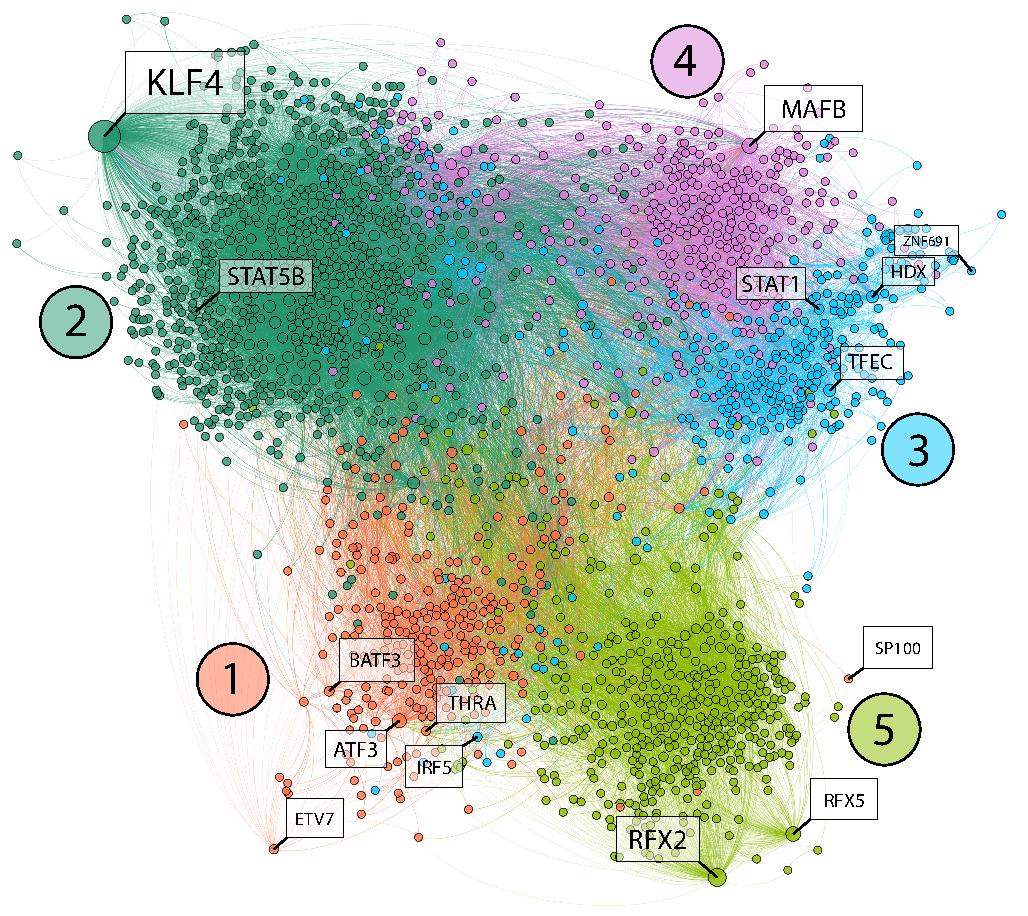
\includegraphics[width=\textwidth]{figures/cd14-ffl-modules}
\caption[Complete Feedforward Loop Network of Differentially Expressed Transcription Factors in CD14-positive Monocytes.]{\textbf{Complete Feedforward Loop Network of Differentially Expressed Transcription Factors in CD14-positive Monocytes.} 
\label{fig:cd14-ffl-modules}}
\end{figure}

\subsubsection{Module One}
GO enrichment analysis of significantly DE genes from module one resulted in 16 GO terms from 35 DE genes. The most significant biological process governed by module one is »negative regulation of transcription« with eight significant genes (SGs) and an adjusted p-value of \e{1.6}{-4}. The second and third terms indicate an influence on apoptotic processes (p = 0.0021 and 0.0049) with three SGs, which are a subset of genes from the first term, \emph{SP100}, \emph{SKIL}, and \emph{ATF3}. Further, module one genes are implicated in positive regulation of GTPase activity (5 SGs, p = 0.0069), epithelial cell differentiation (5 SGs, p = 0.0088), cellular response to IFN-$\upgamma$ (2 SGs, p = 0.024), platelet degranulation (2 SGs, p = 0.033), and cellular response to IL-1 (2 SGs, p = 0.049).

Apart from \emph{SP100} (major constituent of PML-SP100 bodies, see module three), \emph{SKIL} (part of SMAD pathway, regulating cell growth and differentiation), and \emph{ATF3} (member of the broadly acting CREB family of transcription factors), frequently implicated genes include \emph{CCL2} (chemokine ligand for CCR2, exhibits chemotactic activity for monocytes and basophils but not neutrophils and eosinophils pubmed 8627182,9792674,8195247) and \emph{CAMK1} (broadly acting calmodulin-dependent protein kinase, involved e.g. in the ERK cascade).

\subsubsection{Module Two}
Module two, being the largest module, predictably also offers most process-related terms (50 GO terms, 34 DE genes), of which most are related to immunity or basic processes of cell physiology. For the sake of clarity, immunity terms will be explored first. Module two genes most significantly participate in regulation of response to cytokine stimulus (4 SGs, p = \e{2.9}{-4}), response to LPS (5 SGs, p = \e{5.6}{-4}), inflammatory response (6 SGs, p = 0.0015), and T- and B-cell differentiation (2 SGs each, p = 0.036 and 0.041). The highest DE genes from module two involved in these processes are \emph{SORL1} (a known regulator of neurokine signalling), \emph{STAT5B}, the IL-10 receptor $\upalpha$, \emph{PLXNB2} (involved in cell migration),  \emph{JAK2}, the transcription factor \emph{KLF4} (), \emph{PTPN2} (phosphatase involved in dephosphorylating JAKs and STATs), and \emph{CXCL10} (pro-inflammatory chemokine ligand implicated in response to brain injury by activating microglia).
 
Non-immune physiological terms refer to regulation of cell migration (8 SGs, p = \e{1.4}{-4}), negative regulation of MAPK cascade (4 SGs, p = \e{4.7}{-4}), cellular response to peptide (5 SGs, p = \e{9.5}{-4}), nucleus organisation (3 SGs, p = 0.0010), erythrocyte differentiation (3 SGs, p = 0.0010), regulation of ERK cascade (3 SGs, p = 0.0085), regulation of angiogenesis ( SGs, p = 0.0010), regulation of cold-induced thermogenesis (2 SGs, p = 0.031) and several more basic processes. Many of these processes appear to be vital to the immune functions described above, as they share many of the most highly DE genes, such as \emph{SORL1}, \emph{STAT5B}, \emph{PLXNB4}, \emph{KLF4}, and \emph{PTPN2}. Thus, module two genes seem to be responsible for facilitating an adequate immune response by modifying basic processes to enable immune cells to fulfil their functions (e.g., response to cytokines and cellular mobility). 
 
\subsubsection{Module Three}
Module three, with 14 GO terms and 13 DE genes, appears similar in principle to module two, although much fewer basic physiological terms are involved. The most significant biological processes of module two genes involve cellular response to IFN-$\upgamma$ (3 SGs, p = \e{1.6}{-4}) and positive regulation of transcription (5 SGs, p = \e{9.1}{-4}), as opposed to negative regulation of transcription (most significant term in module one). Further, module three genes are involved in the cytokine-mediated signalling pathway (4 SGs, p = 0.0018), regulation of IFN production (2 SGs, p = 0.0034), JAK-STAT cascade (2 SGs, p = 0.0048), negative regulation of angiogenesis (2 SGs, p = 0.0056), regulation of innate immune response (2 SGs, p = 0.035), and positive regulation of cytokine production (2 SGs, p = 0.048). Most frequently occurring genes are \emph{STAT1} and \emph{STAT2}, \emph{PLSCR1} (implicated in amplification of IFN response), \emph{PML} (also associated with IFN- and TNF-responses), and \emph{IRF5} (implicated in TLR7/8-induced induction of IFNs and other pro-inflammatory cytokines).

Mediation of pro-inflammatory cytokine signals via JAK/STAT, opposing module one?

\subsubsection{Module Four}
Module four, with 12 significant GO terms from 7 DE genes, is a fairly small module, which is nevertheless highly associated with immune processes; most significantly, genes of module four convey positive regulation of innate immune response (2 SGs, p = 0.0039) and positive regulation of cytokine production (2 SGs, p = 0.0075). More accurately, they are involved in IL-1 production (1 SG, p = 0.038). Further, module four genes show association with negative regulation of myeloid cell differentiation (1 SG, p = 0.038), positive regulation of response to cytokine (1 SG, p = 0.038), myeloid cell homeostasis (1 SG, p = 0.042), positive regulation of inflammatory response (1 SG, p = 0.045), and negative regulation of myeloid leukocyte differentiation (1 SG, p = 0.049). The most important DE genes in these terms are \emph{GBP5} (activator of the NLRP3 inflammasome assembly), \emph{MAFB} (transcription factor required for monocyte differentiation), and \emph{ZBP1} (cytoplasmic DNA-sensor which activates downstream IFN production in activated macrophages). 
 


\subsubsection{Module Five}
Module five is a medium-sized module (29 GO terms from 18 DE genes) which is only loosely associated with immunity. Most terms relate to basic molecular functions of the cell, such as regulation of cell-substrate adhesion, cellular component maintenance, membrane depolarisation, regulation of protein tyrosine kinase activation, positive regulation of small molecule metabolism, fatty acid metabolic process, and several more. The genes most highly implicated in these processes are \emph{SRC} (tyrosine kinase activated by immune response receptors, that facilitates immune response, adhesion and migration, and apoptosis), \emph{ABCD1} (ATP-binding cassette transporter for very-long-chain fatty acids, implicated in regulation of inflammatory response by positively regulating peroxisomal beta-oxidation), and \emph{HDAC7} (histone deacetylase, in association with RARA has been shown to suppress hsa-miR-10a and thereby influence inflammatory response pubmed28167758).
 
General implications, broad spectrum

%
%\section{Dimensionality Reduction and Correlation of Expression with Clinical Parameters}
%
%\begin{method}
%
%\subsection{WGCNA}
%Reduction of dimensionality of high-dimensional data, such as the expression of thousands of small RNA species and their correlation with clinical parameters of patients, can also be achieved by means of Weighted Gene Correlation Network Analysis (WGCNA, also R/WGCNA).\cite{Langfelder2008} The aim of this method is the identification of modules that group similarly-expressed genes. Each of these modules is represented by an eigenvector (called \emph{eigengene}), effectively replacing the individual expression parameters of the genes in the module. The eigengene can then be used to determine correlation of covariates to each module.
%
%To represent expression data in a network-based manner, the expression matrix is transformed into an adjacency matrix representing similarities between nodes, i.e., genes. The co-expression similarity $s_{ij}$ between two nodes $i$ and $j$ is defined as the absolute correlation coefficient between the expression profiles $$s_{ij} = |cor(x_i, x_j)|$$ with $x$ representing the node expression profile. A signed co-expression measure can be used to keep track of the direction of co-expression. Weighted networks allow the adjacency measures to assume continuous values between 0 and 1, thereby retaining the continuous nature of the underlying expression matrix. This is achieved by implementation of a soft threshold, which is usually chosen by the user to result in a scale-free network topology. The connectivity distribution in a scale-free network follows a power law, i.e., the probability of a node with $k$ connections is, for large values of $k$: $$P(k) = k^{-\alpha}$$ With $\alpha$ usually between 2 and 3. Many biological networks are assumed to be scale-free; however, this assumption has very recently been empirically questioned.\cite{Broido2019}
%
%Once the network is created, modules are identified via unsupervised clustering of densely connected nodes. Biological significance can then be assigned to each of the modules and genes. Module eigengenes can be calculated (the first principal component of the module) and correlated to traits, such as clinical parameters. In this manner, modules with potential functional implications can be identified.
%
%\subsection{Co-correlation}
%The fact that a subset of small \ac{seq} samples were also subjected to large \ac{seq} enables the application of a secondary correlation between those two approaches. For instance, module eigengenes derived from \ac{smrna} analysis can be correlated with the mRNA module eigengenes across the common patients. The module similarity $\sigma$ thus is defined as the correlation coefficient between eigengene profiles $e$ of modules $i$ and $j$: $$\sigma = |cor(e_i, e_j)|$$
%
%Significantly correlating modules (p < 0.05) were identified and further analysed downstream.
%
%%\section{Direct Interaction}
%
%\end{method}
%
%


%!TEX root = ../dissertation.tex
\begin{savequote}[75mm]
If the human brain were so simple that we could understand it, we would be so simple that we couldn’t.
\qauthor{Emerson M. Pugh}
\end{savequote}

\chapter{Discussion}

\newthought{Lorem ipsum dolor sit amet}, consectetuer adipiscing elit. Morbi commodo, ipsum sed pharetra gravida, orci magna rhoncus neque, id pulvinar odio lorem non turpis. Nullam sit amet enim. Suspendisse id velit vitae ligula volutpat condimentum. Aliquam erat volutpat. Sed quis velit. Nulla facilisi. Nulla libero. Vivamus pharetra posuere sapien. Nam consectetuer. Sed aliquam, nunc eget euismod ullamcorper, lectus nunc ullamcorper orci, fermentum bibendum enim nibh eget ipsum. Donec porttitor ligula eu dolor. Maecenas vitae nulla consequat libero cursus venenatis. Nam magna enim, accumsan eu, blandit sed, blandit a, eros.

\section{Methods} \label{sec:discussion:methods}
cell model, chat anomaly, regulation of expression of these two, induction, low vs high control genes
Quisque facilisis erat a dui. Nam malesuada ornare dolor. Cras gravida, diam sit amet rhoncus ornare, erat elit consectetuer erat, id egestas pede nibh eget odio. Proin tincidunt, velit vel porta elementum, magna diam molestie sapien, non aliquet massa pede eu diam. Aliquam iaculis. Fusce et ipsum et nulla tristique facilisis. Donec eget sem sit amet ligula viverra gravida. Etiam vehicula urna vel turpis. Suspendisse sagittis ante a urna. Morbi a est quis orci consequat rutrum. Nullam egestas feugiat felis. Integer adipiscing semper ligula. Nunc molestie, nisl sit amet cursus convallis, sapien lectus pretium metus, vitae pretium enim wisi id lectus. Donec vestibulum. Etiam vel nibh. Nulla facilisi. Mauris pharetra. Donec augue. Fusce ultrices, neque id dignissim ultrices, tellus mauris dictum elit, vel lacinia enim metus eu nunc.

\section{The Cholinergic/Neurokine Interface}
Hypothesis: cholinergic and neurokine systems intermingle significantly in the cns, affecting physiological as well as pathogenic (pathologic?) processes. Multiple angles reject null

\section{Small RNA Therapeutics and Pharmacology} \label{sec:discussion:therapy}
Extant approaches, methods, diseases, PCSK9, asthma, using small RNA antisense as substitute for single-target small molecules, reduce off-target effects, side effects of a different kind

Transcriptomics as basis for selection and design of antisense therapy, combinatorial, compare dirty drugs from psychiatric disorders, serendipity impossible, determinant is the sequence as opposed to functional groups that can be iteratively modified (only 4 building blocks)

%!TEX root = ../dissertation.tex
\chapter{Conclusion}
\label{conclusion}
The study of small RNA dynamics is greatly facilitated by modern bioinformatic methods that enable an understanding of complex transcriptional events in unprecedented detail. While the application and integration of the diverse sources characterising interactions and the participating molecules still are prone to error and misinterpretation, the field advances in giant steps. In summary, the dissertation here presented contributes to the field the following findings:

\begin{itemize}[noitemsep, leftmargin=.5cm, label={\tiny\raisebox{.5ex}{\textbullet}}]
\item Establishment of a framework for the fast and efficient computation of complex interactions between smRNAs, transcription factors, and target genes, including high-resolution tissue specific effects, and on the scale of the whole genome and all miRNAs and tRFs simultaneously;

\item (Re-)establishment of an \emph{in vitro} human cellular model for the study of cholinergic neurons with regard to sex specific phenomena, and, particularly, the effect of neurokine differentiation on cholinergic processes;

\item In this context, elucidation of the potential impact of small RNA dynamics in psychiatric diseases;

\item Identification of pertinent mechanisms in the response to stroke of blood-borne human cells, and interactions between small and large transcripts in these cells;

\item Identification of a neuro-immune axis connecting neurokine mechanisms and cholinergic signalling in multiple instances;

\item Exploration of the feasibility and practicality of feedforward loop analyses, in general and in an example of CD14$^+$ monocytes in post-stroke blood samples;

\item Description of a first step in utilising advanced network approaches for data science in the life sciences, for instance by implementing a »smart« dimensionality reduction.
\end{itemize}


\setstretch{\dnormalspacing}

%bibliography
\clearpage
\addcontentsline{toc}{chapter}{Bibliography}
\bibliography{library, manual_bib}
\bibliographystyle{mystyle}

% articles with multiple URLs have to be manually arranged in library.bib using »note = "\url{}"«
% maybe better just remove all but one URL

\clearpage
\addcontentsline{toc}{chapter}{List of Figures}
\listoffigures

%\clearpage
%\addcontentsline{toc}{chapter}{List of Tables}
%\listoftables

%appendix
\appendix
%!TEX root = ../dissertation.tex
\chapter{Transcription Factor Regulatory Circuits - Tissue Types} 
\label{appendix:marbach}
%!TEX root = ../dissertation.tex
\chapter{List of Primate-Specific Homologues of Human microRNAs} 
\label{appendix:homologues}
\include{chapters/appendix_de-mirs}
%!TEX root = ../dissertation.tex
\chapter{List of GO Terms from Analysis of Differentially Expressed Large RNA in Stroke} 
\label{appendix:go-terms-large-rna}
% latex table generated in R 3.5.1 by xtable 1.8-4 package
% Wed May 13 20:06:09 2020

\noindent \textbf{Abbreviations.} A: Number of Annotated Genes in Term; S: Number of Significant Genes in Term; E: Number of Expected Significant Genes in Term; P: Adjusted P-Value; LFC: log$_2$ fold change.

\vspace{20pt}
 
% latex table generated in R 3.5.1 by xtable 1.8-4 package
% Wed May 13 20:11:59 2020
\begin{table}[ht]
\centering
\begin{tabular}{llcccl}
\multicolumn{6}{c}{\bf Ranking by Count-change, Absolute} \\

  \hline
GO.ID & Term & A & S & E & P \\ 
  \hline
GO:0035456 & response to interferon-beta &  16 &   6 & 0.86 & 1.1E-04 \\ 
  GO:0071346 & cellular response to interferon-gamma &  66 &  12 & 3.57 & 1.4E-04 \\ 
  GO:0035455 & response to interferon-alpha &  13 &   5 & 0.70 & 3.8E-04 \\ 
  GO:0007005 & mitochondrion organization &  63 &   9 & 3.40 & 5.6E-03 \\ 
  GO:0042775 & mitochondrial ATP synthesis coupled elec... &  15 &   4 & 0.81 & 6.9E-03 \\ 
  GO:0050691 & regulation of defense response to virus ... &  15 &   4 & 0.81 & 6.9E-03 \\ 
  GO:0070670 & response to interleukin-4 &  15 &   4 & 0.81 & 6.9E-03 \\ 
  GO:0046427 & positive regulation of JAK-STAT cascade &  16 &   4 & 0.86 & 8.8E-03 \\ 
  GO:0032069 & regulation of nuclease activity &  10 &   3 & 0.54 & 1.4E-02 \\ 
  GO:0045648 & positive regulation of erythrocyte diffe... &  10 &   3 & 0.54 & 1.4E-02 \\ 
  GO:0010469 & regulation of signaling receptor activit... &  38 &   6 & 2.05 & 1.4E-02 \\ 
  GO:0097696 & STAT cascade &  32 &   7 & 1.73 & 2.2E-02 \\ 
  GO:0008285 & negative regulation of cell proliferatio... &  95 &  10 & 5.13 & 2.4E-02 \\ 
  GO:0033273 & response to vitamin &  12 &   3 & 0.65 & 2.4E-02 \\ 
  GO:0050806 & positive regulation of synaptic transmis... &  12 &   3 & 0.65 & 2.4E-02 \\ 
  GO:0001936 & regulation of endothelial cell prolifera... &  21 &   4 & 1.13 & 2.4E-02 \\ 
  GO:0051100 & negative regulation of binding &  32 &   5 & 1.73 & 2.6E-02 \\ 
  GO:0043393 & regulation of protein binding &  44 &   6 & 2.38 & 2.8E-02 \\ 
  GO:0042157 & lipoprotein metabolic process &  13 &   3 & 0.70 & 2.9E-02 \\ 
  GO:0046677 & response to antibiotic &  56 &   7 & 3.03 & 4.1E-02 \\ 
  GO:0048167 & regulation of synaptic plasticity &  15 &   3 & 0.81 & 4.3E-02 \\ 
  GO:0009617 & response to bacterium & 125 &  11 & 6.75 & 4.4E-02 \\ 
  GO:0002576 & platelet degranulation &  37 &   5 & 2.00 & 4.6E-02 \\ 
  GO:0009410 & response to xenobiotic stimulus &  26 &   4 & 1.41 & 4.8E-02 \\ 
   \hline
\end{tabular}
\label{Count-change, Absolute}
\end{table}

% latex table generated in R 3.5.1 by xtable 1.8-4 package
% Wed May 13 20:11:59 2020
\begin{table}[ht]
\centering
\begin{tabular}{llcccl}
\multicolumn{6}{c}{\bf Ranking by Count-change, Negative} \\
  \hline
GO.ID & Term & A & S & E & P \\ 
  \hline
GO:0006954 & inflammatory response &  97 &  15 & 4.99 & 1.3E-04 \\ 
  GO:0042981 & regulation of apoptotic process & 217 &  25 & 11.16 & 1.8E-04 \\ 
  GO:0051241 & negative regulation of multicellular org... & 153 &  19 & 7.87 & 2.9E-04 \\ 
  GO:0032963 & collagen metabolic process &  14 &   5 & 0.72 & 4.5E-04 \\ 
  GO:0046718 & viral entry into host cell &  21 &   6 & 1.08 & 4.6E-04 \\ 
  GO:0030198 & extracellular matrix organization &  29 &   7 & 1.49 & 4.7E-04 \\ 
  GO:0050663 & cytokine secretion &  36 &   9 & 1.85 & 6.8E-04 \\ 
  GO:0051048 & negative regulation of secretion &  32 &   7 & 1.65 & 8.9E-04 \\ 
  GO:0007186 & G protein-coupled receptor signaling pat... &  52 &   9 & 2.67 & 1.0E-03 \\ 
  GO:0032101 & regulation of response to external stimu... &  99 &  16 & 5.09 & 1.1E-03 \\ 
  GO:0002479 & antigen processing and presentation of e... &  17 &   5 & 0.87 & 1.2E-03 \\ 
  GO:1901136 & carbohydrate derivative catabolic proces... &  42 &   8 & 2.16 & 1.3E-03 \\ 
  GO:0070228 & regulation of lymphocyte apoptotic proce... &  12 &   4 & 0.62 & 2.4E-03 \\ 
  GO:0010038 & response to metal ion &  48 &   8 & 2.47 & 2.5E-03 \\ 
  GO:0050671 & positive regulation of lymphocyte prolif... &  20 &   5 & 1.03 & 2.7E-03 \\ 
  GO:0008630 & intrinsic apoptotic signaling pathway in... &  14 &   4 & 0.72 & 4.4E-03 \\ 
  GO:0071236 & cellular response to antibiotic &  23 &   5 & 1.18 & 5.2E-03 \\ 
  GO:0046635 & positive regulation of alpha-beta T cell... &  16 &   4 & 0.82 & 7.4E-03 \\ 
  GO:1904064 & positive regulation of cation transmembr... &  16 &   4 & 0.82 & 7.4E-03 \\ 
  GO:0001776 & leukocyte homeostasis &  25 &   5 & 1.29 & 7.6E-03 \\ 
  GO:0070555 & response to interleukin-1 &  25 &   5 & 1.29 & 7.6E-03 \\ 
  GO:0007565 & female pregnancy &  26 &   5 & 1.34 & 9.0E-03 \\ 
  GO:0030218 & erythrocyte differentiation &  17 &   4 & 0.87 & 9.3E-03 \\ 
  GO:1901222 & regulation of NIK/NF-kappaB signaling &  17 &   4 & 0.87 & 9.3E-03 \\ 
  GO:0006898 & receptor-mediated endocytosis &  48 &   7 & 2.47 & 9.9E-03 \\ 
  GO:0043123 & positive regulation of I-kappaB kinase/N... &  48 &   7 & 2.47 & 9.9E-03 \\ 
  GO:0048771 & tissue remodeling &  27 &   5 & 1.39 & 1.1E-02 \\ 
  GO:0009617 & response to bacterium &  83 &  10 & 4.27 & 1.2E-02 \\ 
  GO:0032731 & positive regulation of interleukin-1 bet... &  10 &   3 & 0.51 & 1.2E-02 \\ 
  GO:0062013 & positive regulation of small molecule me... &  10 &   3 & 0.51 & 1.2E-02 \\ 
  GO:0042542 & response to hydrogen peroxide &  28 &   5 & 1.44 & 1.2E-02 \\ 
  GO:0044092 & negative regulation of molecular functio... & 149 &  16 & 7.66 & 1.4E-02 \\ 
  GO:0010595 & positive regulation of endothelial cell ... &  19 &   4 & 0.98 & 1.4E-02 \\ 
  GO:0051208 & sequestering of calcium ion &  19 &   4 & 0.98 & 1.4E-02 \\ 
  GO:0045807 & positive regulation of endocytosis &  29 &   5 & 1.49 & 1.4E-02 \\ 
   \hline
\end{tabular}
\end{table}
  
\begin{table}  
\begin{tabular}{llcccl}
\multicolumn{6}{c}{\bf Ranking by Count-change, Negative (continued)} \\
  \hline
GO.ID & Term & A & S & E & P \\ 
  \hline
  GO:0050706 & regulation of interleukin-1 beta secreti... &  11 &   3 & 0.57 & 1.6E-02 \\ 
  GO:0032760 & positive regulation of tumor necrosis fa... &  20 &   4 & 1.03 & 1.7E-02 \\ 
  GO:0045582 & positive regulation of T cell differenti... &  20 &   4 & 1.03 & 1.7E-02 \\ 
  GO:0043901 & negative regulation of multi-organism pr... &  25 &   7 & 1.29 & 1.9E-02 \\ 
  GO:0042060 & wound healing &  65 &   9 & 3.34 & 2.0E-02 \\ 
  GO:0032414 & positive regulation of ion transmembrane... &  12 &   3 & 0.62 & 2.1E-02 \\ 
  GO:0071621 & granulocyte chemotaxis &  12 &   3 & 0.62 & 2.1E-02 \\ 
  GO:1901565 & organonitrogen compound catabolic proces... & 230 &  20 & 11.82 & 2.1E-02 \\ 
  GO:0070372 & regulation of ERK1 and ERK2 cascade &  32 &   5 & 1.65 & 2.2E-02 \\ 
  GO:0043069 & negative regulation of programmed cell d... & 138 &  14 & 7.09 & 2.4E-02 \\ 
  GO:0006955 & immune response & 391 &  49 & 20.10 & 2.4E-02 \\ 
  GO:0071356 & cellular response to tumor necrosis fact... &  33 &   5 & 1.70 & 2.4E-02 \\ 
  GO:0010811 & positive regulation of cell-substrate ad... &  13 &   3 & 0.67 & 2.6E-02 \\ 
  GO:0043370 & regulation of CD4-positive, alpha-beta T... &  13 &   3 & 0.67 & 2.6E-02 \\ 
  GO:0070231 & T cell apoptotic process &  13 &   3 & 0.67 & 2.6E-02 \\ 
  GO:1903034 & regulation of response to wounding &  23 &   4 & 1.18 & 2.7E-02 \\ 
  GO:0097237 & cellular response to toxic substance &  34 &   5 & 1.75 & 2.7E-02 \\ 
  GO:0001910 & regulation of leukocyte mediated cytotox... &  14 &   3 & 0.72 & 3.2E-02 \\ 
  GO:0021987 & cerebral cortex development &  14 &   3 & 0.72 & 3.2E-02 \\ 
  GO:0045637 & regulation of myeloid cell differentiati... &  48 &   6 & 2.47 & 3.4E-02 \\ 
  GO:0000209 & protein polyubiquitination &  49 &   6 & 2.52 & 3.7E-02 \\ 
  GO:0001501 & skeletal system development &  49 &   6 & 2.52 & 3.7E-02 \\ 
  GO:0002709 & regulation of T cell mediated immunity &  15 &   3 & 0.77 & 3.8E-02 \\ 
  GO:0006342 & chromatin silencing &  15 &   3 & 0.77 & 3.8E-02 \\ 
  GO:0032392 & DNA geometric change &  15 &   3 & 0.77 & 3.8E-02 \\ 
  GO:0032608 & interferon-beta production &  15 &   3 & 0.77 & 3.8E-02 \\ 
  GO:0051262 & protein tetramerization &  15 &   3 & 0.77 & 3.8E-02 \\ 
  GO:0002495 & antigen processing and presentation of p... &  26 &   4 & 1.34 & 4.1E-02 \\ 
  GO:0006906 & vesicle fusion &  26 &   4 & 1.34 & 4.1E-02 \\ 
  GO:0032088 & negative regulation of NF-kappaB transcr... &  16 &   3 & 0.82 & 4.5E-02 \\ 
  GO:0035265 & organ growth &  16 &   3 & 0.82 & 4.5E-02 \\ 
  GO:0043666 & regulation of phosphoprotein phosphatase... &  16 &   3 & 0.82 & 4.5E-02 \\ 
  GO:0050731 & positive regulation of peptidyl-tyrosine... &  16 &   3 & 0.82 & 4.5E-02 \\ 
  GO:0045185 & maintenance of protein location &  27 &   4 & 1.39 & 4.6E-02 \\ 
  GO:0030855 & epithelial cell differentiation &  54 &   8 & 2.78 & 4.7E-02 \\ 
   \hline
\end{tabular}
\label{Count-change, Negative}
\end{table}

% latex table generated in R 3.5.1 by xtable 1.8-4 package
% Wed May 13 20:11:59 2020
\begin{table}[ht]
\centering
\begin{tabular}{llcccl}
\multicolumn{6}{c}{\bf Ranking by Count-change, Positive} \\
  \hline
GO.ID & Term & A & S & E & P \\ 
  \hline
GO:0033273 & response to vitamin &  12 &   4 & 0.61 & 2.3E-03 \\ 
  GO:0002576 & platelet degranulation &  31 &   6 & 1.57 & 3.8E-03 \\ 
  GO:0042775 & mitochondrial ATP synthesis coupled elec... &  14 &   4 & 0.71 & 4.2E-03 \\ 
  GO:0030324 & lung development &  17 &   4 & 0.86 & 8.9E-03 \\ 
  GO:0008037 & cell recognition &  18 &   4 & 0.91 & 1.1E-02 \\ 
  GO:0009410 & response to xenobiotic stimulus &  28 &   5 & 1.42 & 1.2E-02 \\ 
  GO:0042445 & hormone metabolic process &  19 &   4 & 0.96 & 1.3E-02 \\ 
  GO:0070527 & platelet aggregation &  19 &   4 & 0.96 & 1.3E-02 \\ 
  GO:0046677 & response to antibiotic &  53 &   7 & 2.69 & 1.6E-02 \\ 
  GO:0060348 & bone development &  31 &   5 & 1.57 & 1.8E-02 \\ 
  GO:0001503 & ossification &  43 &   6 & 2.18 & 1.9E-02 \\ 
  GO:0048705 & skeletal system morphogenesis &  22 &   4 & 1.12 & 2.2E-02 \\ 
  GO:0019915 & lipid storage &  13 &   3 & 0.66 & 2.5E-02 \\ 
  GO:0060996 & dendritic spine development &  13 &   3 & 0.66 & 2.5E-02 \\ 
  GO:0099173 & postsynapse organization &  14 &   3 & 0.71 & 3.1E-02 \\ 
  GO:0060271 & cilium assembly &  25 &   4 & 1.27 & 3.5E-02 \\ 
  GO:0061448 & connective tissue development &  25 &   4 & 1.27 & 3.5E-02 \\ 
  GO:0006325 & chromatin organization & 113 &  10 & 5.74 & 3.6E-02 \\ 
  GO:0051604 & protein maturation &  37 &   5 & 1.88 & 3.6E-02 \\ 
  GO:0010595 & positive regulation of endothelial cell ... &  15 &   3 & 0.76 & 3.7E-02 \\ 
  GO:0070670 & response to interleukin-4 &  15 &   3 & 0.76 & 3.7E-02 \\ 
  GO:0007507 & heart development &  50 &   6 & 2.54 & 4.0E-02 \\ 
  GO:0007160 & cell-matrix adhesion &  38 &   5 & 1.93 & 4.0E-02 \\ 
  GO:0060359 & response to ammonium ion &  16 &   3 & 0.81 & 4.4E-02 \\ 
  GO:0030198 & extracellular matrix organization &  39 &   5 & 1.98 & 4.4E-02 \\ 
  GO:0009636 & response to toxic substance &  81 &   8 & 4.11 & 4.6E-02 \\ 
  GO:0045596 & negative regulation of cell differentiat... &  81 &   9 & 4.11 & 5.0E-02 \\ 
   \hline
\end{tabular}
\label{Count-change, Positive}
\end{table}

% latex table generated in R 3.5.1 by xtable 1.8-4 package
% Wed May 13 20:11:59 2020
\begin{table}[ht]
\centering
\begin{tabular}{llcccl}
\multicolumn{6}{c}{\bf Ranking by P-value, Absolute, LFC > 1.4} \\
  \hline
GO.ID & Term & A & S & E & P \\ 
  \hline
GO:0001819 & positive regulation of cytokine producti... &  66 &  14 & 4.38 & 1.7E-04 \\ 
  GO:0032479 & regulation of type I interferon producti... &  29 &   8 & 1.93 & 3.9E-04 \\ 
  GO:0001818 & negative regulation of cytokine producti... &  51 &  11 & 3.39 & 5.7E-04 \\ 
  GO:0009617 & response to bacterium &  95 &  18 & 6.31 & 5.9E-04 \\ 
  GO:0045087 & innate immune response & 151 &  38 & 10.03 & 2.0E-03 \\ 
  GO:0098586 & cellular response to virus &  15 &   5 & 1.00 & 2.1E-03 \\ 
  GO:0046683 & response to organophosphorus &  22 &   6 & 1.46 & 2.3E-03 \\ 
  GO:0002753 & cytoplasmic pattern recognition receptor... &  10 &   4 & 0.66 & 2.8E-03 \\ 
  GO:0048661 & positive regulation of smooth muscle cel... &  16 &   5 & 1.06 & 2.9E-03 \\ 
  GO:0060760 & positive regulation of response to cytok... &  16 &   5 & 1.06 & 2.9E-03 \\ 
  GO:0014074 & response to purine-containing compound &  23 &   6 & 1.53 & 3.0E-03 \\ 
  GO:0032649 & regulation of interferon-gamma productio... &  17 &   5 & 1.13 & 3.8E-03 \\ 
  GO:0016525 & negative regulation of angiogenesis &  12 &   4 & 0.80 & 6.0E-03 \\ 
  GO:0034446 & substrate adhesion-dependent cell spread... &  13 &   4 & 0.86 & 8.3E-03 \\ 
  GO:0032496 & response to lipopolysaccharide &  46 &   8 & 3.06 & 9.2E-03 \\ 
  GO:0009063 & cellular amino acid catabolic process &  14 &   4 & 0.93 & 1.1E-02 \\ 
  GO:0031349 & positive regulation of defense response &  58 &  11 & 3.85 & 1.2E-02 \\ 
  GO:0002576 & platelet degranulation &  22 &   5 & 1.46 & 1.3E-02 \\ 
  GO:0010469 & regulation of signaling receptor activit... &  49 &   8 & 3.26 & 1.3E-02 \\ 
  GO:0070887 & cellular response to chemical stimulus & 404 &  54 & 26.84 & 1.6E-02 \\ 
  GO:0030168 & platelet activation &  32 &   6 & 2.13 & 1.6E-02 \\ 
  GO:0034109 & homotypic cell-cell adhesion &  16 &   4 & 1.06 & 1.8E-02 \\ 
  GO:0050731 & positive regulation of peptidyl-tyrosine... &  25 &   5 & 1.66 & 2.2E-02 \\ 
  GO:0048469 & cell maturation &  17 &   4 & 1.13 & 2.2E-02 \\ 
  GO:0097696 & STAT cascade &  17 &   4 & 1.13 & 2.4E-02 \\ 
  GO:0043330 & response to exogenous dsRNA &  10 &   3 & 0.66 & 2.4E-02 \\ 
  GO:0071695 & anatomical structure maturation &  18 &   4 & 1.20 & 2.7E-02 \\ 
  GO:0050680 & negative regulation of epithelial cell p... &  19 &   4 & 1.26 & 3.3E-02 \\ 
  GO:0007267 & cell-cell signaling & 146 &  11 & 9.70 & 3.5E-02 \\ 
  GO:0001936 & regulation of endothelial cell prolifera... &  20 &   4 & 1.33 & 3.9E-02 \\ 
  GO:0006906 & vesicle fusion &  20 &   4 & 1.33 & 3.9E-02 \\ 
  GO:0007160 & cell-matrix adhesion &  20 &   4 & 1.33 & 3.9E-02 \\ 
  GO:0030856 & regulation of epithelial cell differenti... &  12 &   3 & 0.80 & 4.0E-02 \\ 
  GO:0034113 & heterotypic cell-cell adhesion &  12 &   3 & 0.80 & 4.0E-02 \\ 
  GO:0042130 & negative regulation of T cell proliferat... &  12 &   3 & 0.80 & 4.0E-02 \\ 
  GO:0051668 & localization within membrane &  12 &   3 & 0.80 & 4.0E-02 \\ 
   \hline
\end{tabular}
\label{P-value, LFC > 1.4, Absolute}
\end{table}

% latex table generated in R 3.5.1 by xtable 1.8-4 package
% Wed May 13 20:11:59 2020
\begin{table}[ht]
\centering
\begin{tabular}{llcccl}
\multicolumn{6}{c}{\bf Ranking by P-value, Negative, LFC > 1.4} \\
  \hline
GO.ID & Term & A & S & E & P \\ 
  \hline
GO:0051607 & defense response to virus &  44 &  10 & 2.72 & 2.2E-04 \\ 
  GO:0019221 & cytokine-mediated signaling pathway & 110 &  16 & 6.80 & 7.8E-04 \\ 
  GO:0035270 & endocrine system development &  10 &   4 & 0.62 & 2.2E-03 \\ 
  GO:0006511 & ubiquitin-dependent protein catabolic pr... &  74 &  11 & 4.57 & 2.6E-03 \\ 
  GO:0042102 & positive regulation of T cell proliferat... &  17 &   5 & 1.05 & 2.8E-03 \\ 
  GO:0000209 & protein polyubiquitination &  42 &   8 & 2.60 & 3.3E-03 \\ 
  GO:0034341 & response to interferon-gamma &  42 &   8 & 2.60 & 3.3E-03 \\ 
  GO:0002831 & regulation of response to biotic stimulu... &  18 &   5 & 1.11 & 3.7E-03 \\ 
  GO:0045786 & negative regulation of cell cycle &  70 &  10 & 4.33 & 3.8E-03 \\ 
  GO:0050658 & RNA transport &  31 &   6 & 1.92 & 4.5E-03 \\ 
  GO:0006513 & protein monoubiquitination &  13 &   4 & 0.80 & 6.4E-03 \\ 
  GO:0045071 & negative regulation of viral genome repl... &  14 &   4 & 0.87 & 8.5E-03 \\ 
  GO:0071347 & cellular response to interleukin-1 &  14 &   4 & 0.87 & 8.5E-03 \\ 
  GO:0016032 & viral process & 108 &  15 & 6.67 & 2.0E-02 \\ 
  GO:0043900 & regulation of multi-organism process &  53 &  11 & 3.28 & 2.5E-02 \\ 
  GO:1902533 & positive regulation of intracellular sig... & 110 &  14 & 6.80 & 2.6E-02 \\ 
  GO:0034097 & response to cytokine & 156 &  23 & 9.64 & 2.8E-02 \\ 
  GO:0001819 & positive regulation of cytokine producti... &  61 &   8 & 3.77 & 3.1E-02 \\ 
  GO:0030855 & epithelial cell differentiation &  57 &   8 & 3.52 & 3.3E-02 \\ 
  GO:0032663 & regulation of interleukin-2 production &  12 &   3 & 0.74 & 3.4E-02 \\ 
  GO:0035264 & multicellular organism growth &  12 &   3 & 0.74 & 3.4E-02 \\ 
  GO:0051865 & protein autoubiquitination &  12 &   3 & 0.74 & 3.4E-02 \\ 
  GO:0044265 & cellular macromolecule catabolic process & 148 &  20 & 9.15 & 3.6E-02 \\ 
  GO:0018107 & peptidyl-threonine phosphorylation &  13 &   3 & 0.80 & 4.2E-02 \\ 
  GO:0048469 & cell maturation &  13 &   3 & 0.80 & 4.2E-02 \\ 
  GO:0032103 & positive regulation of response to exter... &  32 &   5 & 1.98 & 4.3E-02 \\ 
  GO:0008285 & negative regulation of cell proliferatio... &  80 &  10 & 4.94 & 4.8E-02 \\ 
   \hline
\end{tabular}
\label{P-value, LFC > 1.4, Negative}
\end{table}

% latex table generated in R 3.5.1 by xtable 1.8-4 package
% Wed May 13 20:11:59 2020
\begin{table}[ht]
\centering
\begin{tabular}{llcccl}
\multicolumn{6}{c}{\bf Ranking by P-value, Positive, LFC > 1.4} \\
  \hline
GO.ID & Term & A & S & E & P \\ 
  \hline
GO:0010594 & regulation of endothelial cell migration &  20 &   5 & 0.87 & 1.2E-03 \\ 
  GO:0006939 & smooth muscle contraction &  13 &   4 & 0.56 & 1.7E-03 \\ 
  GO:0090257 & regulation of muscle system process &  28 &   5 & 1.21 & 6.0E-03 \\ 
  GO:0002478 & antigen processing and presentation of e... &  20 &   4 & 0.87 & 9.3E-03 \\ 
  GO:0016358 & dendrite development &  20 &   4 & 0.87 & 9.3E-03 \\ 
  GO:0016525 & negative regulation of angiogenesis &  11 &   3 & 0.48 & 1.0E-02 \\ 
  GO:0022904 & respiratory electron transport chain &  11 &   3 & 0.48 & 1.0E-02 \\ 
  GO:0048041 & focal adhesion assembly &  11 &   3 & 0.48 & 1.0E-02 \\ 
  GO:0002040 & sprouting angiogenesis &  12 &   3 & 0.52 & 1.3E-02 \\ 
  GO:0030193 & regulation of blood coagulation &  12 &   3 & 0.52 & 1.3E-02 \\ 
  GO:0046034 & ATP metabolic process &  23 &   4 & 1.00 & 1.5E-02 \\ 
  GO:0006898 & receptor-mediated endocytosis &  35 &   5 & 1.52 & 1.6E-02 \\ 
  GO:0001936 & regulation of endothelial cell prolifera... &  13 &   3 & 0.56 & 1.6E-02 \\ 
  GO:1902600 & proton transmembrane transport &  13 &   3 & 0.56 & 1.6E-02 \\ 
  GO:0050900 & leukocyte migration &  60 &   6 & 2.60 & 2.0E-02 \\ 
  GO:0097305 & response to alcohol &  25 &   4 & 1.08 & 2.1E-02 \\ 
  GO:0043434 & response to peptide hormone &  43 &   5 & 1.86 & 2.6E-02 \\ 
  GO:0007611 & learning or memory &  27 &   4 & 1.17 & 2.7E-02 \\ 
  GO:0051048 & negative regulation of secretion &  29 &   4 & 1.26 & 2.9E-02 \\ 
  GO:0007584 & response to nutrient &  16 &   3 & 0.69 & 2.9E-02 \\ 
  GO:0034622 & cellular protein-containing complex asse... & 115 &  10 & 4.98 & 2.9E-02 \\ 
  GO:0051897 & positive regulation of protein kinase B ... &  18 &   3 & 0.78 & 4.0E-02 \\ 
  GO:0050730 & regulation of peptidyl-tyrosine phosphor... &  31 &   4 & 1.34 & 4.2E-02 \\ 
  GO:0016571 & histone methylation &  19 &   3 & 0.82 & 4.6E-02 \\ 
   \hline
\end{tabular}
\label{P-value, LFC > 1.4, Positive}
\end{table}


%!TEX root = ../dissertation.tex
\chapter{Examples of Presence/Absence Definition of Small RNA} 
\label{appendix:presence-absence}


% the back matter
% \backmatter



% \include{endmatter/colophon}

\end{document}
